\PassOptionsToPackage{full}{textcomp}
% include symmetric to place margins left and right instead of right only
% nohyper, nobib?
\documentclass[nobib,a4paper,twoside,notoc,justified,marginals=justified]{tufte-book}
\hypersetup{colorlinks}
\usepackage[utf8]{inputenc}

% fix too many alphabets error
\usepackage{amsmath, amssymb}
\newcommand\hmmax{0}
\newcommand\bmmax{0}

% fix margins?
% \usepackage{marginfix}

\usepackage{enumitem, bm, xcolor, braket, dsfont, graphicx, cancel}
% \usepackage[colorlinks, linkcolor = red, citecolor = black, filecolor = black, urlcolor = blue]{hyperref} 
% \usepackage{nameref}
% \hypersetup{colorlinks}
\usepackage{algorithmic}

% Quotes
\usepackage{epigraph}
\setlength\epigraphwidth{10cm}
\setlength\epigraphrule{0pt}

%% style
% \usepackage{mathptmx}
% \usepackage{setspace}
% \linespread{1.0}

% \iflarger
%\AtBeginDocument{%
%	\fontsize{12}{14}\selectfont
%}%
% \else\fi


% integrate amsthm and txmath
\usepackage{savesym}
\usepackage{amsthm}
\savesymbol{openbox}
\usepackage{newtxtext,newtxmath}
\restoresymbol{TX}{openbox}

% theorems
\newtheorem*{theorem}{Theorem}
\newtheorem*{thm}{Theorem}

% shorthand
\renewcommand{\t}[1]{\text{#1}}
\renewcommand{\d}{{\rm d}}
\renewcommand{\b}[1]{{\bf #1}}
\newcommand{\B}[1]{\mathbf{#1}}
\newcommand{\D}[1]{{#1}^\dagger}
\newcommand{\fD}[1]{{#1}^{ \phantom{\dagger}}}
\renewcommand{\P}[1]{{#1}^\prime}
\newcommand{\fP}[1]{{#1}^{\phantom{\prime}}}
\newcommand{\im}{{\rm i}}
\newcommand{\halb}{\frac{1}{2}}
\DeclareMathOperator{\Tr}{Tr}
\newcommand{\kb}{k_{\rm B}}

% transpose
\usepackage{relsize}
\newcommand{\tp}[1]{{#1}^{\mathrm t}}
% \!\: = 1mu distance; \!\; = 2mu (\, = 3mu)
\newcommand{\itp}[1]{{#1}^{\!\:\scalebox{0.55}[1.0]{\( - \)}1 \mathrm t}}

% comments:
\definecolor{dblue}{RGB}{31,119,180}
\newcommand{\REM}[1]{\textcolor{red}{{\bf #1}}}
\newcommand{\CITE}[1]{\textcolor{dblue}{{\bf [CITE: #1]}}}
% \newcommand{\FK}[1]{\textcolor{blue}{{\bf #1 }}}

% Tufte

% TOC
% https://tex.stackexchange.com/questions/121790/how-to-generate-a-full-width-table-of-contents-tufte-book
\usepackage{lipsum,mdframed}
\definecolor{secnum}{RGB}{13,151,225}
\definecolor{ptcbackground}{RGB}{212,237,252}
\definecolor{ptctitle}{RGB}{0,177,235}

\setcounter{secnumdepth}{3}

\usepackage[toc]{appendix}
% \usepackage{titletoc}
% \usepackage{etoolbox}
\setcounter{tocdepth}{1}
%\pretocmd{\tableofcontents}{\begin{mdframed}\let\cleardoublepage\relax}{}{}
%  \apptocmd{\tableofcontents}{\end{mdframed}}{}{}

% The fancyvrb package lets us customize the formatting of verbatim
% environments.  We use a slightly smaller font.
\usepackage{fancyvrb}
\fvset{fontsize=\normalsize}

%%
% Prints argument within hanging parentheses (i.e., parentheses that take
% up no horizontal space).  Useful in tabular environments.
\newcommand{\hangp}[1]{\makebox[0pt][r]{(}#1\makebox[0pt][l]{)}}

%%
% Prints an asterisk that takes up no horizontal space.
% Useful in tabular environments.
\newcommand{\hangstar}{\makebox[0pt][l]{*}}

%%
% Prints a trailing space in a smart way.
\usepackage{xspace}

% Prints the month name (e.g., January) and the year (e.g., 2008)
\newcommand{\monthyear}{%
  \ifcase\month\or January\or February\or March\or April\or May\or June\or
  July\or August\or September\or October\or November\or
  December\fi\space\number\year
}


% Prints an epigraph and speaker in sans serif, all-caps type.
\newcommand{\openepigraph}[2]{%
  %\sffamily\fontsize{14}{16}\selectfont
  \begin{fullwidth}
  \sffamily\large
  \begin{doublespace}
  \noindent\allcaps{#1}\\% epigraph
  \noindent\allcaps{#2}% author
  \end{doublespace}
  \end{fullwidth}
}

% Inserts a blank page
\newcommand{\blankpage}{\newpage\hbox{}\thispagestyle{empty}\newpage}

\usepackage{units}

% Typesets the font size, leading, and measure in the form of 10/12x26 pc.
\newcommand{\measure}[3]{#1/#2$\times$\unit[#3]{pc}}

% Macros for typesetting the documentation
\newcommand{\hlred}[1]{\textcolor{Maroon}{#1}}% prints in red
\newcommand{\hangleft}[1]{\makebox[0pt][r]{#1}}
\newcommand{\hairsp}{\hspace{1pt}}% hair space
\newcommand{\hquad}{\hskip0.5em\relax}% half quad space
\newcommand{\TODO}[1]{\textcolor{red}{\bf TODO: {#1}}\xspace}
\newcommand{\na}{\quad--}% used in tables for N/A cells

% Generates the index
\usepackage{makeidx}
\makeindex


\begin{document}

  % Front matter
  \frontmatter
  
%  % r.1 blank page
%  \blankpage
%  
%% r.3 full title page
%\maketitle

% r.5 contents
\tableofcontents

% \listoffigures

% \listoftables

% r.7 dedication
%\cleardoublepage
%~\vfill
%\begin{doublespace}
%  \noindent\fontsize{12}{12}\selectfont\itshape
%  \nohyphenation
%  \hfill To my teachers.
%\end{doublespace}
%\vfill
%\vfill


% r.9 introduction
\cleardoublepage
\addtocontents{toc}{\protect\setcounter{tocdepth}{0}}
\chapter{Introduction}
\epigraph{\singlespacing \it ``Die Zeit des unbedenklichen Wirtschaftens mit den Energiequellen und Stofflagern, die uns die Natur zur Verfügung gestellt hat, wird wahrscheinlich schon für unsere Kinder nur noch die Bedeutung einer vergangenen Wirtschaftsepoche haben.''}{W. Schottky, 1929~\cite{Schottky1929}}
% [ ] Why thermal conductivity?
% [ ] Why novel thermal insulators?
% [ ] Why computational materials science?
\newthought{One of the major challenges} humankind faces in the 21th century is the responsible and sustainable handling of the earth's natural resources.  Yet, most energy today is lost as waste heat during the transformation of raw energy sources to usable power. To date, there is no fuel based heat engine that exceeds an efficiency of 50\,\% and often it is even worse~\cite{eia}. 
Since gas- and aircraft-turbines are essentially Carnot engines, their efficiency and core power are directly related to the combustion temperature~\cite{Clarke2012,Perepezko2009}. This has been utilized during the past 30 years by developing 
ceramics with high thermal resistivity that are nowadays applied as \emph{thermal barrier coatings} on turbine airfoils in heat engines~\cite{Clarke2003}. A thermal barrier coating serves as a thin, extremely heat insulating layer and thus allows to operate a turbine at higher temperatures, thereby increasing its efficiency.

A complementary strategy is to recycle waste heat where it occurs. One way to do so is to use the
\emph{thermoelectric effect} to  generate electric power from temperature gradients~\cite{Snyder2008}. The main obstacle preventing mass operation though is the limited conversion rate (figure of merit) $zT$ of even the most advanced thermoelectric materials known to date. To make matters worse, these materials often contain heavy metals and are toxic, and their manufacturing process is difficult and expensive~\cite{Nolas2001}. Recent advancements in the field, such as the discovery of a high thermoelectric figure of merit in the lead-free material Tin Selenide~\cite{Zhao2014}, offer hope that novel materials with significant figure of merit can be found that are non-toxic, easy and cheap to produce, and consist of abundant elements.

\newthought{A key physical property} of both thermal barrier coatings (TBCs) and thermoelectrics is their thermal conductivity $\kappa$. In the case of thermoelectrics, the figure of merit is inversely proportional to $\kappa$~\cite{Nolas2001}:
\begin{align}
zT = \frac{S^2 \sigma_{\rm el}}{\kappa} T~,
\label{eq:zT}
\end{align} 
where $T$ dentoes the temperature, $S$ the Seebeck coefficient, and $\sigma_{\rm el}$ is the electrical conductivity.
A prerequisite to finding better thermoelectrics or TBCs therefore is to find materials which are thermally insulating. These are typically non-metals, since the free electrons in metals are good heat carriers, and most of the known thermoelectrics are thermally insulating inorganic semiconductors~\cite[p.\,15]{Nolas2001}.

% [ ] say sth. about microstructuring?

Despite the technological needs, systematic knowledge of thermal conductivities in inorganic compounds is scarce. A renowned database like Springer Materials only lists thermal conductivities for about 200~of these compounds~\cite{SpringerMaterials}, which is partially due to the fact that accurate measurements of thermal conductivity are tricky to perform[\REM{citation!}]. As a consequence, thermal conductivity is not systematically understood beyond semi-empirical and phenomenological trends in a very limited number of simple material classes~\cite{Morelli}.

\newthought{The aim of this work} is to open a new pathway for overcoming the problem of limited data by devising a route to systematically scan material space for thermal insulators and calculate their thermal conductivities from first principles. This route is twofold: After reviewing the relevant theoretical tools necessary to simulate heat transport in thermal insulators, we describe how to assess a key physical property shared by most thermal insulators,~.i.\,e.,~\emph{anharmonicity}, without the need for explicit model building beyond the harmonic approximation.

\section*{Organization of the Thesis}
\TODO{Derive all the formulas, discuss anharmonicity, present thermal conductivity}

%%
% Start the main matter (normal chapters)
\mainmatter

\addtocontents{toc}{\protect\setcounter{tocdepth}{2}}
\part{Theory and Methods}

\chapter{The Many Body Problem}
\epigraph{\singlespacing \it ``The underlying physical laws necessary
for the mathematical theory of a large part of physics and the whole of chemistry
are thus completely known, and the difficulty is only that the exact application
of these laws leads to equations much too complicated to be soluble. It therefore becomes desirable that approximate practical methods of applying quantum
mechanics should be developed, which can lead to an explanation of the main
features of complex atomic systems without too much computation.''}{P.A.M. Dirac, 1929}

In this chapter, we summarize the theoretical background of {\it ab initio} simulations.

\subsection{The Many Body Hamiltonian}

The full (non-relativistic) many body Hamiltonian in the absence of external electromagnetic fields for an otherwise arbitrary system reads
\begin{align}
    \hat{\mathrm{H}}
        = \hat{\mathrm{T}}^{\mathrm{e}}
        + \hat{\mathrm{V}}^{\mathrm{e}-\mathrm{e}}
        + \hat{\mathrm{V}}^{\mathrm{e}-\mathrm{Nuc}}
        + \hat{\mathrm{V}}^{\mathrm{Nuc}-\mathrm{Nuc}}
        + \hat{\mathrm{T}}^{\mathrm{Nuc}}~,
    \label{eq:Hamiltonian}
\end{align}
where
\begin{align}
    \hat T^{\rm e} 
        =\sum_{i} \frac{\hat{\mathbf{p}}_{i}^{2}}{2 m_{\rm e}}
    \label{eq:Te}
\end{align}
is the kinetic energy operator for electrons of mass $m_{\rm e}$ with momentum operators $\hat{\bf p}_i$, and 
\begin{align}
    \hat V^{\rm e-e}
        = \sum_{i < j} \frac{e^{2}}{\left|\hat{\b r}_{i}-\hat{\bf r}_{j}\right|}~,
    \label{eq:Ve}
\end{align}
is the Coulombic electron-electron repulsion operator with the electronic position operators $\hat{\bf r}_i$ and the elementary charge $e$. 
The Coulomb attraction between the negatively charged electrons and the positively charged nuclei reads
\begin{align}
    \hat V^{\rm e-Nuc}
        = \sum_{i, J} -\frac{Z_J e^{2}}{\left|\hat{\b r}_{i}-\hat{\bf R}_{J}\right|}~,
    \label{eq:Venuc}
\end{align}
where $Z_J$ denotes the charge number of nucleus $J$, and $\hat{\bf R}_J$ is the nuclear position operator. 
Accordingly, we define the nuclear-nuclear repulsion as
\begin{align}
    \hat V^{\rm Nuc-Nuc}
        = \sum_{I < J} \frac{Z_{I} Z_{J} e^{2}}{\left|\hat{\b R}_{I}-\hat{\bf R}_{J}\right|}~,
    \label{eq:Vnuc}
\end{align}
and the kinetic energy operator for nuclei with momentum operators $\hat{\bf P}_I$ and masses $M_I$ reads
\begin{align}
    \hat T^{\rm Nuc} 
        =\sum_{I} \frac{\hat{\mathbf{P}}_{I}^{2}}{2 M_{I}}~.
    \label{eq:Tnuc}
\end{align}

\subsection{The Born Oppenheimer Approximation}
We go over to a unitless Hamiltonian by scaling Eq.\,\eqref{eq:Hamiltonian} with the Hartree energy $E_{\rm h} = me^4 / \hbar^2 \approx 27.2\,{\rm eV}$ and expressing distances in terms of the Bohr radius $a_0 = \hbar^2 / m e^2$,~i.\,e.,~${\bf r} = a_0 \tilde{\bf r}$, where $\hbar$ denotes the Planck constant~\CITE{Czycholl}. Dropping the operator hats in the following and using $\hat{\bf p}=-\im \hbar \partial / \partial {\bf r}$ instead, we have
\begin{align}
\begin{split}
    \tilde H 
        \equiv& ~H / E_{\rm h} \\
        =& 
        - \frac{1}{2} \sum_i \frac{\partial^2}{\partial \tilde{\bf r}_i^2}
        + \sum_{i < j} \frac{1}{\left|\tilde{\b r}_{i}-\tilde{\bf r}_{j}\right|}
        - \sum_{i, J} -\frac{Z_J}{\left|\tilde{\b r}_{i}-\tilde{\bf R}_{J}\right|}
        + \sum_{I < J} \frac{Z_{I} Z_{J}}{
            \left|\tilde{\b R}_{I}-\tilde{\bf R}_{J}\right|} 
        \\
        &- \frac{1}{2} \sum_I \frac{m_{\rm e}}{M_I} \frac{\partial^2}{\partial \tilde{\bf R}_I^2}~,
    \label{eq:Hscaled}
\end{split}
\end{align}
which only depends on the charge numbers $\{Z_I\}$ and the mass ratios $\{ m_{\rm e} / M_I \}$. The relative order of magnitude of the nuclear kinetic energy is $m_{\rm e} / M_I \approx 10^{-4} - 10^{-5}$. This means that the nuclear kinetic energy can be treated as a perturbation of the remaining electronic and electron-nuclear contributions:
\begin{align}
    H   &= H^0 + T^{\rm Nuc}~, \text{ where} 
    \label{eq:H=H0+T}
    \\
    H^0 &=
        {\mathrm{T}}^{\mathrm{e}}
        + {\mathrm{V}}^{\mathrm{e}-\mathrm{e}}
        + {\mathrm{V}}^{\mathrm{e}-\mathrm{Nuc}}
        + {\mathrm{V}}^{\mathrm{Nuc}-\mathrm{Nuc}}~.
    \label{eq:H0}
\end{align}
The full (time-independent) many-body Schroedinger equation reads
\begin{align}
    H \psi ({\bf r}, {\bf R}) = E \psi ({\bf r}, {\bf R})~,
    \label{eq:Schroedinger1}
\end{align}
with ground-state eigenvalues and many-body wave functions $E$ and \mbox{$\psi ({\bf r}, {\bf R})$},
where \mbox{${\bf r} = ({\bf r}_, \ldots, {\bf r}_{N_{\rm e}})$} denotes all electronic coordinates, and ${\bf R} = ({\bf R}_1, \ldots, {\bf R}_{N_{\rm Nuc}})$ all nuclear coordinates, respectively. According to Eq.\,\eqref{eq:H=H0+T}, we expand the wave functions $\psi ({\bf r}, {\bf R})$ in a complete set of orthonormal basis functions $\phi_l$,
\begin{align}
\psi ({\bf r}, {\bf R}) = \sum_l \chi_l ({\bf R}) \phi_l ({\bf r}, {\bf R})~,
\label{eq:psi_expansion_phi}
\end{align}
where the $\phi_l$ are the solutions to the Hamiltonian $H^0$,
\begin{align}
    H^0 \phi_l ({\bf r}, {\bf R})
        = E^0_l ({\bf R}) \phi_l ({\bf r}, {\bf R})~.
    \label{eq:Hsolution1}
\end{align}
The dependence of $\phi_l$ and the eigenvalue $E_l^0({\bf R})$ on $\bf R$ is parametric,~i.\,e.,~Eq.\,\eqref{eq:Hsolution1} is solved for a given nuclear configuration $\bf R$.

The functions $\chi_l$ are to be determined by using Eq.\,\eqref{eq:psi_expansion_phi} in Eq.\,\eqref{eq:Schroedinger1},
\begin{align}
    (H - E) \psi ({\bf r}, {\bf R})
        & = \sum_l (H^0 + T^{\rm Nuc} - E) \chi_l ({\bf R}) \phi_l ({\bf r}, {\bf R}) \nonumber \\
        &= \sum_l (E^0_l({\bf R}) + T^{\rm Nuc} - E) \chi_l ({\bf R}) \phi_l ({\bf r}, {\bf R}) \\
    = 0 \nonumber~,
\end{align}
and integrating with $\int \d^3 r ~ \phi^\ast_m ({\bf r}, {\bf R})$ using their orthonormality, so that
\begin{align}
    \left( T^{\rm Nuc} + E^0_m({\bf R}) \right) \chi_m ({\bf R})
        + \sum_l C_{ml} ({\bf R}) \chi_l ({\bf R})
        = E \chi_m ({\bf R})~,
    \label{eq:chi1}
\end{align}
where the operator $C_{ml}$~\CITE{Czycholl},
\begin{align}
    C_{ml} ({\bf R})
        = - \sum_I \frac{\hbar^2}{2 M_I} \int \d^3 r ~ 
        &\left[ \phi^\ast_m ({\bf r}, {\bf R}) \frac{\partial^2}{\partial {\bf R}_I^2}
            \phi_l ({\bf r}, {\bf R}) \right. \nonumber \\
        &\left.
            + 2 \phi^\ast_m ({\bf r}, {\bf R}) \left(
                \frac{\partial}{\partial {\bf R}_I} \phi_l ({\bf r}, {\bf R}) \right)
            \frac{\partial}{\partial {\bf R}_I}
        \right]~,
    \label{eq:Aml}
\end{align}
describes coupling between different electronic states $(l, m)$. This term is of the order of $(m/M)^{1/4} \approx 10^{-1} - 10^{-2}$ smaller than the nuclear energy~\cite{BornOppenheimer}. Neglecting this term is known as the \emph{Born-Oppenheimer approximation} and completely separates the dynamical evolution of electrons and nuclei. In effect, Eq.\,\eqref{eq:chi1} reduces to
\begin{align}
    \left( T^{\rm Nuc} + E^0_l({\bf R}) \right) \chi_l ({\bf R})
        = E \chi_l ({\bf R})~.
    \label{eq:chi2}
\end{align}
Solving Eq.\,\eqref{eq:chi2} is performed in two steps:
\begin{enumerate}
    \item For a given configuration $\bf R$, the electronic Schr\"odinger equation \eqref{eq:Hsolution1} is solved, yielding the energies $E^0_l({\bf R})$ which thereby parametrically depend on $\bf R$.
    \item For each electronic quantum number $l$, Eq.\,\eqref{eq:chi2} for the nuclei is solved, where the electronic energy $E^0_l({\bf R})$ defines the effective \emph{potential energy surface}.
\end{enumerate}
Pictorially, the electrons move \emph{adiabatically} with the nuclei.\footnote{Born and Oppenheimer neglected $C_{ml}$ in their original work~\cite{BornOppenheimer} and later called this the \emph{adiabatic approximation}~\cite{BornHuang}. However, only the terms $C_{m \neq l}$ describe a coupling of different electronic states induced by nuclear coupling, and keeping the terms $C_{m=l}$ gives the exact potential when the electronic states are sufficiently separated,~e.\,g.,~in presence of an electronic gap~\cite{BornHuang}. Therefore the term ``adiabatic approximation'' is nowadays used when only the terms $C_{m=l}$ are kept~\cite{Marx2009}. The full BO approximation is correct to fourth order in the expansion of the full Hamiltonian in the mass parameter $\sqrt[4]{m/M}$~\cite{BornHuang}.} Since we will deal with insulators and semiconductors with bandgaps providing a sufficient energetic separation between the electronic ground state $l=0$ and the first exited state $l=1$,\footnote{Thermal energy at room temperature is $\sim 25\,{\rm meV} \ll $~typical bandgap.} we will concentrate on the electronic ground state energy $E^0_0$ for the given configuration ${\bf R}$ in the following. We denote this energy as the \emph{Born-Oppenheimer potential energy},
\begin{align}
	E^{\rm BO} ({\bf R}) \equiv E^0_0 ({\bf R})~.
	\label{eq:E^BO}
\end{align}

\subsection{Density Functional Theory}
\epigraph{\singlespacing \it ``It is my sense that at the present time DFT is the method of choice for systems consisting of many (\,$\gtrsim 5$) atoms and for smaller systems, when moderate accuracies are sufficient.''}{W.~Kohn, 1993}

In the previous chapter, it was tacitly assumed that the electronic Schr\"odinger equation \eqref{eq:Hsolution1} yielding the effective potential for the nuclei can be solved. Finding an exact solution to this equation is, however, infeasible for more than a few electrons. We will now introduce \emph{density functional theory} (DFT) as a framework for making approximations that enable to find a first-principles electronic potential energy surface $E^{\rm BO} ({\bf R})$ for atomic systems with order of magnitudes more electrons.

To set the stage, we rewrite the electronic Schr\"odinger equation \eqref{eq:Hsolution1}:
\begin{align}
	\hat H = \hat T + \hat W + \hat V^{\rm ext}~,
	\label{eq:H.dft.1}
\end{align}
where $T \equiv T^{\rm e}$ denotes the electronic kinetic energy operator, $W \equiv V^{\rm e-e}$ is the electronic Coulomb repulsion, and $V^{\rm ext} \equiv V^{\rm e-Nuc}$ is the \emph{external} potential determined by the nuclear configuration $\bf R$. Note that the bare nuclear-nuclear repulsion $V^{\rm Nuc-Nuc}$ is neglected as it merely contributes an additive constant to the electronic Hamiltonian at fixed configuration and therefore does not change the solutions to Eq.\,\eqref{eq:H.dft.1}.

Let us look for solutions to Eq.\,\eqref{eq:H.dft.1} of the form
\begin{align}
	\hat H \Ket{\Psi} = E_\Psi \Ket{\Psi}~,
	\label{eq:SE.dft.1}
\end{align}
where $\hat H$ is the electronic Hamiltonian given by Eq.\,\eqref{eq:H.dft.1}, $\Ket{\Psi}$ denotes a many-body eigenstate in index-free bra--ket notation\footnote{
	Here and in the following we employ the usual convention that from the state $\Ket{\Psi}$, many-body wavefunctions are obtained via
	\begin{align*}
		\braket{{\bf r} | \Psi} 
			= \Psi ({\bf r})
		\Leftrightarrow
		\braket{{\bf r}_1, \ldots, {\bf r}_N | \Psi} 
			= \Psi({\bf r}_1, \ldots, {\bf r}_N)~.
	\end{align*}
	Likewise we define the $\mathcal{L}^2$ scalar product as
	$$
	\braket{\Psi | \Phi} = \int \d^{3N} r ~ \Psi^\ast ({\bf r}) \ \Phi({\bf r})~.
	$$	
},
and $E_\Psi$ is the corresponding total energy.

Any state $\Ket{\Psi}$ maps to an electron density $n_\Psi ({\bf x})$ via the density operator
\begin{align}
	\hat n ({\bf x}) \equiv \sum_i \hat n_i ({\bf x}) = \sum_i \delta ({\bf x} - \hat{\bf r}_i)~,
	\label{eq:densop}
\end{align}
such that
\begin{align}
	n_\Psi({\bf x}) 
	\equiv \Braket{\Psi | \hat n({\bf x}) | \Psi} 
	= N \int \d^3 r_2 \cdots \d^3 r_{N} ~ 
	\left\lvert 
	\Psi ({\bf x}, {\bf r}_2, \ldots, {\bf r}_N) 
	\right\rvert^2~,
\end{align}
where it was used that the arguments of $\lvert \Psi ({\bf r}_1, \ldots, {\bf r}_N) \rvert^2$ can be arbitrarily permuted.
We note that ${\bf x} \in \mathds{R}^3$ denotes a point in real space, whereas ${\bf r} = ({\bf r}_1, \ldots, {\bf r}_N)$ denotes the positions of electrons as before.
%\begin{align}
%	\braket{\Psi | n_i({\bf r}) | \Psi} 
%		= \int \d^3 r_1 \cdots \d^3 r_{i-1} \d^3 r_{i+1} \cdots \d^3 r_{N} ~ 
%			\left\lvert 
%				\Psi ({\bf r}_1, \ldots, {\bf r}_{i-1}, {\bf x}, {\bf r}_{i+1}, \ldots, {\bf r}_N) 
%			\right\rvert^2
%\end{align}
The density operator $\hat n ({\bf x})$ can be used to express the one-particle operator $V^{\rm ext}$ as an operator valued functional of a potential function $v^{\rm ext} ({\bf x})$ by writing
\begin{align}
	\hat V^{\rm ext}
		= \sum_i v^{\rm ext} (\hat{\bf r}_i)
		= \int \d^3 x ~ v^{\rm ext} ({\bf x}) \, \hat n ({\bf x})~,
		\label{eq:Vext}
\end{align}
where $v^{\rm ext} ({\bf x})$ is the Coulomb potential stemming from the nuclear arrangement $\bf R$,~cf.~Eq.\,\eqref{eq:Venuc}.
It follows that the expectation value of Eq.\,\eqref{eq:Vext} is a functional of the density,
\begin{align}
	\braket{\Psi | \hat V^{\rm ext} | \Psi}
		= V^{\rm ext} [n_\Psi]
		= \int \d^3 x ~ v^{\rm ext} ({\bf x}) \, n_\Psi ({\bf x})~.
		\label{eq:dft.Vext.expectation}
\end{align}
As $n_\Psi$ is obtained from the solution $\Ket{\Psi}$ of Eq.\,\eqref{eq:SE.dft.1} and the term $\hat V^{\rm ext}$ in the Hamiltonian given by Eq.\,\eqref{eq:H.dft.1} is solely determined by the external potential funktion $v^{\rm ext} ({\bf x})$ via Eq.\,\eqref{eq:Vext}, it naturally follows that $n_\Psi ({\bf r})$ is a functional of $v^{\rm ext} ({\bf x})$. In other words, there is a map between the set of external potentials $\mathbb V = \set{v^{\rm ext}}$, and the set of eigensolutions $\mathbb P = \set{\Psi}$ and their corresponding densities $\mathbb N = \set{n_\Psi}$:
\begin{align}
	M: \mathbb V \rightarrow \mathbb N~.
	\label{eq:dft.map.1}
\end{align}

\subsubsection{Hohenberg-Kohn}
Hohenberg and Kohn were able to show that, for non-degenerate ground states $\Psi \equiv \Psi_0$, there exists the \emph{inverse map} from ground-state densities $\mathbb N_0$ to potential functions $\mathbb V$, and that this map is bijective~\CITE{HohenbergKohn64}:\footnote{Kohn was later able to loosen the requirement of non-degeneracy~\CITE{Kohn1985}.}
\begin{align}
	M^{-1}: \mathbb N_0 \rightarrow \mathbb V~. 
\end{align}
The beauty of this theorem is that it establishes a one-to-one correspondence between the \emph{ground-state density} $n_0 ({\bf x})$ and the external potential function $v^{\rm ext} ({\bf x})$ which, in turn, describes the full many-body problem via Eq.\,\eqref{eq:H.dft.1}. For example, the ground-state wavefunctions $\Psi_0$ are functionals of $n_0$, as well as the expectation value of any ground-state observable. In the following, we will stay with ground-state densities and denote them simply by $n ({\bf x}) \equiv n_0 ({\bf x})$.

Hohenberg and Kohn further define the \emph{universal functional} 
\begin{align}
	F[n] \equiv \Braket{\Psi [n] | \hat T + \hat W | \Psi [n]}~,
	\label{eq:dft.Fn}
\end{align}
i.\,e.,~the contributions to the Hamiltonian which do not depend on the external potential. The ground-state total energy for a given potential function $v$ is then given as
\begin{align}
	E [n] 
		= \Braket{\Psi [n] | \hat H | \Psi [n]}
		\equiv F[n] + V^{\rm ext}[n]~,
		%+ \int \d^3 x ~ v ({\bf x}) n ({\bf x})~.
	\label{eq:dft.En}
\end{align}
where $V^{\rm ext}[n]$ is given by Eq.\,\eqref{eq:dft.Vext.expectation}.
By virtue of the Raleigh-Ritz variational principle, this functional is minimized for the correct ground-state density $n$ only, and any other density $n'$ that differs from $n$ non-trivially yields a larger energy:
\begin{align}
	E[n] < E [n'] \quad \text{for} \quad n \neq n'~.
\end{align}
This also means that the true ground-state density for a given potential $v$ can be found by minimizing the total energy function, Eq.\,\eqref{eq:dft.En},
\begin{align}
	n = \arg \min_{n} E[n]~,
	\label{eq:dft.n}
\end{align}
under the constraint of fixed particle number imposed by the Lagrange multiplier $\mu$,
%\begin{align}
%	N [n] = \int \d^3 x ~ n({\bf x}) = N~.
%	\label{eq:dft.N}
%\end{align}
%By using Eq.\,\eqref{eq:dft.N}, the total energy can be written as a functional of the external potential $v$ and the particle Number $N$ under the requirement of stationarity,
%\begin{align}
%	\begin{split}
%		E        &= E[v, N] \\
%		\delta E &= 0~,
%	\end{split}
%	\label{eq:dft.stationarity}
%\end{align}
%or, by imposing the conservation of particle number explicitly via the Lagrange multiplicator $\mu$,
\begin{align}
	\frac{\delta}{\delta n ({\bf x})}
		\left.\left[ 
			E[n] + \mu \left(
				\int \d^3 x' ~ n ({\bf x}') - N \right)
		\right]\right\vert_{n = n_0}
		=0~.
		\label{eq:dft.stationarity}
\end{align}

\subsubsection{Reconstructing the Born-Oppenheimer Surface}
In the definition of the effective electronic Hamiltonian in Eq.\,\eqref{eq:H.dft.1}, we had neglected the nuclear repulsion $V^{\rm Nuc-Nuc}$ defined in Eq.\,\eqref{eq:Vnuc}. The Born-Oppenheimer potential energy surface defined in Eq.\,\eqref{eq:E^BO} therefore consists of both terms,~i.\,e.,
\begin{align}
	E^{\rm BO} ({\bf R}) 
		= E[n] + \sum_{I < J} \frac{Z_{I} Z_{J} e^{2}}{\left|{\bf R}_{I}-{\bf R}_{J}\right|}~.
	\label{eq:E^BO}
\end{align}

\subsection{Hellmann-Feynmann Theorem}
The forces on individual atomic positions ${\bf R}_I$ are given in terms of derivatives of the Born-Oppenheimer energy, $E^{\rm BO} ({\bf R})$,
\begin{align}
	\frac{\d}{\d {\bf R}_I} E^{\rm BO} ({\bf R})
		\stackrel{\eqref{eq:E^BO}}{=}
			\frac{\d}{\d {\bf R}_I } \left[
				E[n] + \sum_{J < K} \frac{Z_{J} Z_{K} e^{2}}{\left|{\b R}_{J}-{\bf R}_{K}\right|}
			\right]
			~.
	\label{eq:hellmannfeynman.1}
\end{align}
The electronic part is given by
\begin{align}
		\frac{\d}{\d {\bf R}_I} E[n]
			= 
				\underset{I}{\underbrace{\frac{\partial}{\partial {\bf R}_I} E[n]}}
			+ \underset{II}{\underbrace{
					\int \d^{3} x ~ \frac{\delta E[n]}{\delta n(\boldsymbol{x})} \frac{\partial n(\boldsymbol{x})}{\partial {\bf R}_{I}}
				}}~,
		\label{eq:hellmannfeynman.2}
\end{align}
where term $II)$ can be evaluated under the assumption of stationarity expressed by Eq.\,\eqref{eq:dft.stationarity} which yields 
\mbox{$\delta E[n] / \delta n({\bf x}) = -\mu$},
and using the Leibniz rule, so that
\begin{align}
	\int \d^{3} x ~ \frac{\delta E[n]}{\delta n(\boldsymbol{x})} \frac{\partial n(\boldsymbol{x})}{\partial {\bf R}_{I}}
	= -\mu \frac{\partial}{\partial {\bf R}_I} \int \d^{3} x ~ n ({\bf x})
	= 0~.
	\label{eq:hellmannfeynman.3}
\end{align}
Term $I)$ only depends explicitly on ${\bf R}_I$ via the electron-nucleus contribution to $V^{\rm ext}$ given by Eq.\,\eqref{eq:Venuc}, yielding
\begin{align}
	\frac{\d}{\d {\bf R}_I} E[n]
		= \frac{\d}{\d {\bf R}_I} \braket{\Psi_0 | \hat V ^{\rm ext} | \Psi_0} 
		= \int \d^3 x ~ n({\bf x}) \frac{Z_I e^2 ({\bf R}_I - {\bf x})}{\left\lvert {\bf R}_I - {\bf x} \right\rvert^3}~.
\end{align}
In total, we have
\begin{align}
	\frac{\d}{\d {\bf R}_I} E^{\rm BO} ({\bf R})
	= \int \d^3 x ~ n({\bf x}) \frac{Z_I e^2 ({\bf R}_I - {\bf x})}{\left\lvert {\bf R}_I - {\bf x} \right\rvert^3}
	- \sum_{I \neq J} \frac{Z_I Z_J e^2 ({\b R}_{I}-{\bf R}_{J})}{
		\left\lvert {\bf R}_{I}-{\bf R}_{J} \right\rvert^3}~,
	\label{eq:hellmannfeynman.force}
\end{align}
which is solely determined by the ground-state electron density $n ({\bf x})$ and the nuclear configuration $\bf R$. This result is known as the \emph{Hellmann-Feynman theorem}\CITE{Hellmann, Feynman}, which can also be formulated in more general terms for any parametric dependence of the Hamiltonian on some external quantitiy $\lambda$:
\begin{theorem}[Hellmann-Feynman]
\begin{align}
	\frac{\d E_{\lambda}}{\d \lambda}
		= \frac{\d}{\d \lambda}\left\langle\Psi_{\lambda} \left|\hat{H}_{\lambda}\right| \Psi_{\lambda} \right\rangle
		= \left\langle\Psi_{\lambda} \left| \frac{\d \hat{H}_{\lambda}}{\d \lambda} \right| \Psi_{\lambda} \right\rangle~.
\end{align}
\end{theorem}
We note in passing that while the Hellmann-Feynman theorem is formally correct, in practice there often arise correction terms when non-complete basis sets are used that also depend on the parameter $\lambda$. The most famous correction are the so-called \emph{Pulay forces} that arise in atom centered basissets~\CITE{Pulay1969}.

\subsection{Kohn-Sham Scheme}
By introducing density functional theory, we have not solved the many-body problem. However, we have shifted the intricacies of this problem to a \emph{universal} functional $F[n]$ which depends on the electron density $n({\bf x})$, which is a scalar function of three coordinates, $n: \mathds R^3 \rightarrow \mathds R$, and thus entails a \emph{massive} reduction of complexity compared to working with wavefunctions, which are complex functions of $3N$ variables, $\Psi: \mathds R^{3N} \rightarrow \mathds C$.

In order to proceed, we follow the original argument by Kohn and Sham~\CITE{KohnSham1965} and investigate the universal functional $F[n]$ defined in Eq.\,\eqref{eq:dft.Fn} in more detail. The definition reads
\begin{align}
	F[n] 
		= \Braket{\Psi [n] | \hat T + \hat W | \Psi [n]}
		\equiv T[n] + W[n]~,
	\label{eq:dft.Fn.2}
\end{align}
where $T[n]$ now denotes the kinetic energy of the electrons expressed as a functional of the density $n ({\bf x})$, and $W[n]$ denotes the electron-electron interaction term. We split this term into two contributions,
\begin{align}
	\begin{split}
	W[n] 
		&= E^{\rm es} [n] + E^{\rm xc} [n] \\
		&= \frac{1}{2} \int \mathrm{d}^{3} x ~ 
			v^{\mathrm{es}}[n](\boldsymbol{x}) n(\boldsymbol{x})+E^{\mathrm{xc}}[n]~,
	\end{split}
	\label{eq:dft.KS.W}
\end{align}
where $E^{\rm es} [n]$ is the electrostatic (Hartree) energy stemming from a charge distribution $n ({\bf x})$ in the Coulomb potential
\begin{align}
	v^{\mathrm{es}}[n](\boldsymbol{x})
		= \int \mathrm{d}^{3} x^{\prime} \frac{n\left(\boldsymbol{x}^{\prime}\right)}{\left|\boldsymbol{x}-\boldsymbol{x}^{\prime}\right|}~,
	\label{eq:dft.KS.ves}
\end{align}
which is a functional of the density itself. $E^{\rm xc} [n]$ denotes all exchange and correlation effects not captured by $E^{\rm es} [n]$ and is therefore termed the \emph{exchange-correlation energy}. Again, we have only shifted the problem, this time to the unknown functional $E^{\rm xc} [n]$ which we will discuss later.
In this notation, the total energy functional for the electron system in an external potential reads
\begin{align}
	E[n]
		= T[n] +  E^{\rm es}[n] + E^{\rm xc} [n] + V^{\rm ext}[n]~.
	\label{eq:dft.Ks.En}
\end{align}

Let us now define the density $n({\bf x})$ in terms of an \emph{auxiliary} orthonormal set of complex functions $\{ \psi_l ({\bf x}) \}$, such that
\begin{align}
	n({\bf x}) = \sum_l f_l \left\lvert \psi_l ({\bf x}) \right\rvert^2~,
	\label{eq:dft.KS.n(psi)}
\end{align}
where ${\bf f}=\set{f_l : 0 \leq f_l \leq 1}$ denote the occupation of each orbital,~i.\,e.,~a Fermi-like function that represents a thermal ensemble or the 0\,K ground state. We use Eq.\,\eqref{eq:dft.KS.n(psi)} in Eq.\,\eqref{eq:dft.Ks.En} and vary with respect to $\psi^\ast_l ({\bf x})$ under the constraint of keeping the functions $\set{\psi_l}$ normalized via the Lagrange multiplier $\lambda_l$,
\begin{align}
	\frac{\delta}{\delta \psi^\ast_l ({\bf x})}
		\left[
			T[n] +  E^{\rm es}[n] + E^{\rm xc} [n] + V^{\rm ext}[n]
			- \lambda_l \left(
				\int \d^3 x ~ \left\lvert \psi_l ({\bf x}) \right\rvert^2 - 1
			\right)
		\right]
		= 0~.
	\label{eq:dft.Ks.variation.1}
\end{align}
By Eq.\,\eqref{eq:dft.KS.n(psi)} we have
\begin{align}
	\frac{\delta n({\bf x})}{\delta \psi^\ast_l ({\bf x}')}
		&= f_l \psi_l ({\bf x}) \delta ({\bf x} - {\bf x}')~,
	\label{eq:dft.KS.dn}
\end{align}
and therefore by chain rule 
$\delta / \delta \psi^\ast = (\delta n / \delta \psi^\ast) \delta / \delta n$
%\begin{align}
%	\frac{\delta n({\bf x})}{\delta \psi^\ast_l ({\bf x}')}
%		&= f_l \psi_l ({\bf x}) \delta ({\bf x} - {\bf x}')~,
%		\label{eq:dft.KS.dn} \\
%	\frac{\delta T[n]}{\delta \psi^\ast_l ({\bf x})}
%		&= -\frac{1}{2} f_l \nabla^2 \psi_l ({\bf x})
%		\label{eq:dft.KS.dT} \\
%	\frac{\delta E^{\rm es}[n]}{\delta \psi^\ast_l ({\bf x})}
%		&= v^{\rm es} [n] ({\bf x})
%		\label{eq:dft.KS.dEes} \\
%	\frac{\delta E^{\rm xc}[n]}{\delta \psi^\ast_l ({\bf x})}
%		&= v^{\rm xc} [n] ({\bf x})
%		\label{eq:dft.KS.dExc} \\
%	\frac{\delta v^{\rm ext}[n]}{\delta \psi^\ast_l ({\bf x})}
%		&= v^{\rm ext} ({\bf x})
%		\label{eq:dft.KS.dEext} \\
%\end{align}
\begin{align}
	\left(
		-\frac{1}{2} \nabla^2 
		+ v^{\rm es} [n] ({\bf x})
		+ v^{\rm xc} [n] ({\bf x})
		+ v^{\rm ext}  ({\bf x})
	\right) \psi_l ({\bf x})
	= \frac{\lambda_l}{f_l} \psi_l ({\bf x})~.
	\label{eq:dft.KS.1}
\end{align}
Here, $-\frac{1}{2} \nabla^2$ is the kinetic operator, $v^{\rm es}$ and $v^{\rm ext}$ are the electrostatic and external potentials defined earlier, and
\begin{align}
	v^{\rm xc} [n] ({\bf x})
		= \frac{\delta E^{\rm xc}[n]}{\delta n ({\bf x})}
	\label{eq:dft.vxc}
\end{align}
is the \emph{exchange-correlation potential} formally defined as the functional derivative of $E^{\rm xc} [n]$ with respect to the density. By summarizing the three potentials entering Eq.\,\eqref{eq:dft.KS.1} as one \emph{effective} potential,
\begin{align}
	v^{\rm eff} [n] ({\bf x})
	\equiv
		v^{\rm es} [n] ({\bf x})
		+ v^{\rm xc} [n] ({\bf x})
		+ v^{\rm ext}  ({\bf x})~,
	\label{eq:dft.KS.veff}
\end{align}
 and denoting $\epsilon_l \equiv \lambda_l / f_l$, we can write
\begin{align}
	\left(
		-\frac{1}{2} \nabla^2 
		+ v^{\rm eff} [n] ({\bf x})
	\right) \psi_l ({\bf x})
	= \epsilon_l \psi_l ({\bf x})~,
\label{eq:dft.KS.2}
\end{align}
which is a one-particle Schr\"odinger-like equation for orbitals $\psi_l$ with eigenvalues $\epsilon_l$ in an effective potential $v^{\rm eff}[n]$ which is a functional of the density $n$ given in terms of the orbitals by Eq.\,\eqref{eq:dft.KS.n(psi)}. Equation\,\eqref{eq:dft.KS.2} therefore needs to be solved \emph{self-consistently} by starting from an initial guess for the density $n^0$ to set up the effective potential, and solving for $(\psi_l, \epsilon_l)$ until convergence. That the density $n$ of the \emph{interacting} many-particle systems can be obtained from the \emph{non-interacting} single-particle for the Kohn-Sham orbitals $\psi_l$ is ensured by the \emph{Kohn-Sham theorem}~\CITE{KohnSham1965,GrossDreizler1990}.

Given that the solution $\set{\psi_l, \epsilon_l}$ is known, Eq.\,\eqref{eq:dft.KS.2} can be used to express the kinetic energy in terms of the density and eigenvalues $\epsilon_l$ by summing and integrating with $\sum_l \int \d^3 x~\psi^\ast_l ({\bf x})$ and using the orthonormality of the orbitals $\psi_l$, so that
\begin{align}
	T[n] 
		\equiv - \frac{1}{2}\sum_l \int \d^3 x ~ \psi^\ast_l ({\bf x}) \nabla^2 \psi({\bf x})
		\stackrel{\eqref{eq:dft.KS.2}}{=} 
			\sum_l \epsilon_l 
			- \int \d^3 x ~ v^{\rm eff}[n] ({\bf x}) n({\bf x})~.
	\label{eq:dft.KS.Tn}
\end{align}
The total energy in terms of the Kohn-Sham eigenvalues $\set{\epsilon_l}$ and density $n ({\bf x}) = \sum_l \lvert \psi_l ({\bf x}) \rvert^2$ is then given as
\begin{align}
	E[n]
		&\stackrel{\phantom{\eqref{eq:dft.KS.Tn}}}{=} 
			T[n] 
			+ \frac{1}{2} \int \d^3 x ~ v^{\rm es} [n] ({\bf x}) n ({\bf x})
			+ E^{\rm xc}[n]
			+ \int \d^3 x ~ v^{\rm ext} ({\bf x}) n ({\bf x})
			\nonumber \\
		&\stackrel{\eqref{eq:dft.KS.Tn}}{=}
			\sum_l \epsilon_l 
			- \frac{1}{2} \int \d^3 x ~ v^{\rm es} [n] ({\bf x}) n ({\bf x})
			+ E^{\rm xc}[n]
			- \int \d^3 x ~ v^{\rm xc}[n] ({\bf x}) n ({\bf x})~.
	\label{eq:dft.KS.En}
\end{align}

\subsection{Approximations to the exchange-correlation energy}
\label{sec:dft.approximations}
We are finally in position to introduce approximations to the exchange-correlation energy functional $E^{\rm xc}[n]$ from which the corresponding potential can be obtained by the functional derivative with respect to the density as expressed in Eq.\,\eqref{eq:dft.KS.veff}. Indeed, the very success of the Kohn-Sham DFT scheme probably can be traced back to the fact that simple approximations to $E^{\rm xc}[n]$ lead to reasonable results for a large class of systems. 

Let us now define an exchange-correlation energy density via
\begin{align}
	E^{\rm xc}[n] 
		= \int \d^3 x ~ e^{\rm xc} \left[ n \right] ({\bf x})~,
\label{eq:dft.xc.1}
\end{align}
where the density $e^{\rm xc} \left[ n \right] ({\bf x})$ is a functional of the density by itself. 
The most straighforward way to approximate $e^{\rm xc}[n] ({\bf x})$ is to replace the \emph{functional} $e^{\rm xc} [n] ({\bf x})$ by a \emph{function} of the local density,
\begin{align}
	e^{\rm xc} [n] ({\bf x})
		\approx e^{\rm xc}_{\rm LDA} \left( n({\bf x}) \right)~.
	\label{eq:dft.exc.lda.1}
\end{align}
This approximation is called the \emph{local density approximation} (LDA), and the resulting exchange-correlation energy reads\footnote{
	Some authors prefer to write $e^{\rm xc}(n) = n \tilde e^{\rm xc} (n)$, such that
	\begin{align*}
		E^{\rm xc} = \int \d^3 x ~ n({\bf x}) \tilde e^{\rm xc} (n ({\bf x}))~.
	\end{align*}}
\begin{align}
	E^{\rm xc}_{\rm LDA}[n] 
		= \int \d^3 x ~ e^{\rm xc}_{\rm LDA} \left(n ({\bf x}) \right)~.
	\label{eq:dft.LDA.1}
\end{align}
The energy density $e^{\rm xc}_{\rm LDA} \left(n ({\bf x}) \right)$ is usually taken to be the exchange-correlation energy density of a homogeneous electron gas obtained from higher-level theory approaches. The LDA is (by construction) exact in the limit of vanishing density gradient, $\lvert \nabla n ({\bf x}) \rvert / n({\bf x}) \rightarrow 0$, but yields surprisingly good results under circumstances where the density is non-homogeneous as well.\REM{what does that mean? Chp. 7.2 Gross/Greizler}\CITE{Gross/Dreizler}

In the spirit of the original work by Hohenberg and Kohn, and Kohn and Sham, improvements on the LDA can be constructed by going beyond the local density and taking into account gradients of the density as well,
\begin{align}
	e^{\rm xc} [n] ({\bf x})
		\approx e^{\rm xc}_{\rm GGA} \left( n({\bf x}), \nabla n({\bf x}) \right)~.
	\label{eq:dft.exc.gga.1}
\end{align}
Again, the full functional $e^{\rm xc}[n]$ is replaced by a function of the density and its gradient. This approximation is called \emph{generalized gradient approximation} (GGA), an the resulting energy is usually written in the form
\begin{align}
		E^{\rm xc}_{\rm GGA}[n] 
		= \int \d^3 x ~ e^{\rm x}_{\rm hom} \left(n ({\bf x}) \right) 
			F^{\rm xc} \left(n ({\bf x}), \lvert \nabla n ({\bf x})\rvert \right)~,
		\label{eq:dft.GGA.1}
\end{align}
where $e^{\rm x}_{\rm hom}(n)$ is the exchange energy density of a homogeneous electron gas, and $F^{\rm xc}(n, \nabla n)$ is an \emph{enhancement factor}.
\CITE{[1] J. P. Perdew, J. A. Chevary, S. H. Vosko, K. A. Jackson, M. R. Pederson, D. J. Singh, and C. Fiolhais, Phys. Rev. B 46, 6671 (1992).}
\CITE{[1] J. P. Perdew, K. Burke, and M. Ernzerhof, Phys. Rev. Lett. 77, 3865 (1996).}

\subsection{Periodic Systems}
So far, we did not specify the external potential $v^{\rm ext} ({\bf x})$ entering the Kohn-Sham equation \eqref{eq:dft.KS.1} beyond stating that it describes the arrangement of nuclei. For (finite) molecules and clusters, this is already sufficient and a self-consistent solution to Eq.\,\eqref{eq:dft.KS.1} can be attempted from here. For (practically infinite) bulk systems and crystals on the other hand, further statements need to be made.

Let us assume that the configuration of the nuclei is in a perfect periodic arrangement described by the 
%\emph{unit cell}
%\begin{align}
%	\text{unit cell}
%		= \set{{\bf x} = f^i {\bf a}_i : f^i \in \mathds R^{[0, 1)}}~,
%	\label{eq:dft.Bloch.unitcell}
%\end{align}
%where 
\emph{Bravais vectors}
\begin{align}
	{\bf R}_{\bf n} 
		= \sum_{i=1}^{3} n^i {\bf a}_i~,
	\label{eq:Rn}
\end{align}
where $\set{{\bf a}_i}$ is a basis that spans
the \emph{unit cell},
\begin{align}
	\text{unit cell}
		= \set{{\bf x} = f^i {\bf a}_i : f^i \in \mathds R^{[0, 1)}}~,
	\label{eq:dft.Bloch.unitcell}
\end{align}
and the full crystal is spanned by the unit cell translated by all possible translations $\bf R_n$ given by Eq.\,\eqref{eq:Rn} with integer numbers smaller than some large but finite value $N_i$ for each basis vector ${\bf a}_i$, $\set{n^i : n^i \in \mathds{N}^{[0, N_i)}}$. The periodicity of the crystal is characterized by the condition that any translation by $\bf R_n$ maps the crystal back onto itself such that
\begin{align}
	v^{\rm ext} ({\bf x} + {\bf R_n}) 
		= v^{\rm ext} ({\bf x})~.
	\label{eq:dft.Bloch.1}
\end{align}
By definition of the effective potential entering the Kohn-Sham equations \eqref{eq:dft.KS.2}, $v^{\rm eff} [n] ({\bf x})$ shares this periodicity. We can therefore formulate a \emph{Bloch theorem}\footnote{Cf.~Sec.\,\ref{sec:BlochTheorem} for an informal proof.}
for the Kohn-Sham orbitals $\psi_l ({\bf x})$,~i.\,e.,~solutions to Eq.\,\eqref{eq:dft.KS.2} can be separated into independent equations labelled by a quantum number $\bf k$ with solutions
\begin{align}
	\psi_{{\bf k} l} ({\bf x}) 
		= {\rm e}^{\im {\bf k} \cdot {\bf x}} u_{{\bf k} l} ({\bf x})
	\label{eq:dft.Bloch.2}
\end{align}
where $u_{{\bf k} l}$ are periodic functions satisfying
\begin{align}
	u_{{\bf k} l} ({\bf x} + {\bf R_n})
		= u_{{\bf k} l} ({\bf x})~,
	\label{eq:dft.Bloch.3}
\end{align}
and $\bf k$ is restricted to the first Brillouin zone of the reciprocal lattice.

\subsubsection{Born-von Karman Boundary Conditions}
To ensure normalizability of the functions $\psi_{{\bf k}l}$, one additionally imposes the \emph{Born-von Karman boundary conditions}
\begin{align}
	\psi_{{\bf k}l} ({\bf x} + N_i {\bf a}_i) 
		= \psi_{{\bf k}l} ({\bf x})
	\label{eq:dft.Bloch.4}
\end{align}
where $N_i$ denotes the number of repetitions along direction ${\bf a}_i$. The domain $V$ of all functions and functionals appearing the Kohn-Sham equations thereby becomes a parallelepiped of size 
$V = N_1 N_2 N_3 \, {\bf a}_1 \cdot ({\bf a}_2 \times {\bf a}_3)$ with periodically connected edges. The ideal, infinite crystal is obtained in the limit $N_i \rightarrow \infty$.
Using the periodic boundary condition expressed by Eq.\,\eqref{eq:dft.Bloch.4} in the Bloch functions given by Eq.\,\eqref{eq:dft.Bloch.2}, and the periodicity of the functions $u_{{\bf k} l}$, one finds that
\begin{align}
%	{\rm e}^{\im {\bf k} \cdot ({\bf x} + N_i {\bf a}_i)} u_{{\bf k} l} ({\bf x})
%		&= {\rm e}^{\im {\bf k} \cdot {\bf x}} u_{{\bf k} l} ({\bf x}) \nonumber \\
%	\implies
%		{\rm e}^{\im {\bf k} \cdot  N_i {\bf a}_i} 
%			&= 1 \nonumber \\
%	\implies
		{\bf k} \cdot {\bf a}_i
			&= \frac{2 \pi}{N_i} m_i~,\quad\text{with } m_i \in \mathds N^{[0, N_i)}~.
	\label{eq:dft.Bloch.5}
\end{align}
In total there are $N = N_1 N_2 N_3$ unique values of $\bf k$ labelled by ${\bf m} = (m_1, m_2, m_3)$ that can be expressed in terms of the \emph{reciprocal lattice vectors}~\cite{Sands2002}
\begin{align}
	{\bf b}^i 
		= 2 \pi \varepsilon^{ijk} \frac{{\bf a}_j \times {\bf a}_k}{{\bf a}_1 \cdot ({\bf a}_2 \times {\bf a}_3)} ~,
	\label{eq:dft.Bloch.bi}
\end{align}
where $\varepsilon^{ijk}$ denotes the Levi-Civita symbol enforcing the correct ordering of $ijk$. The complete set of $\bf k$-values is
\begin{align}
	{\bf k}_{\bf m} 
		= \sum_{i=1}^3 \frac{m_i}{N_i} {\bf b}^i~.
	\label{eq:dft.Bloch.k_m}
\end{align}
The space spanned by the $\set{{\bf b}_i}$,~i.\,e.,~the space containing all unique values of $\b k$, is the unit cell of the reciprocal lattice. Alternatively, one chooses those equivalent $\bf k_m$ which are closest to the $\bf 0$,~i.\,e.,~the Brillouin zone. The values of $\bf k$ given by Eq.\,\eqref{eq:dft.Bloch.k_m} are those sampled in real-space simulation in a box of the given size,~i.\,e.,~the \emph{Born-von Karman cell}.

\subsection{Conclusion}
The concept of density functional theory in the Kohn-Sham scheme (KS-DFT) has been presented starting from the general many-body Hamiltonian given in Eq.\,\eqref{eq:Hamiltonian}. Besides the Born-Oppenheimer (BO) approximation which decouples electron and nuclear dynamics, KS-DFT offers a formally exact way of computing the total energy of the electronic ground state from first principles by solving Schr\"odinger-like single-particle equations,~i.\,e.,~the KS equations, for an auxiliary set of functions,~i.\,e.,~the KS-orbitals. In order to solve the KS equations one needs to approximate the exchange-correlation energy, $E^{\rm xc} [n]$. In Sec.\,\ref{sec:dft.approximations} we have introduced the most common approaches to approximate $E^{\rm xc} [n]$,~i.\,e.,~the local-density approximation (LDA), as well as the generalized-gradient approximation (GGA).

Within the BO approximation, the BO potential-energy surface determines all dynamical properties of the nuclear system, for example heat transport. We discuss dynamical properties of this kind in more detail in the next section.

% \newpage

\chapter{Lattice Dynamics}
In the previous chapter, we have seen how the many-body problem can be decoupled into an electronic problem given by Eq.\,\eqref{eq:Hsolution1}, which can be solved in the framework of DFT, and a nuclear problem given by Eq.\,\eqref{eq:chi2} that describes the dynamical properties of the nuclei. This was achieved by means of the Born-Oppenheimer approximation where electron-nucleus interactions beyond a parametric dependence on each other is neglected~\cite{BornOppenheimer}.

We will now introduce two approximations to progress in the description of the nuclear dynamics. First, the \emph{harmonic approximation} in which the nuclear Schr\"odinger equation is solved for an approximated potential. Second, we treat the nuclei as particles, but on the full, non-truncated Born-Oppenheimer potential. This will lead to the formulation of \emph{ab initio molecular dynamics} (aiMD). As no electron will appear anymore, $N \equiv N_{\rm Nuc}$ will henceforth denote the number of nuclei in the system of interest, and we denote the Born-Oppenheimer potential simply as \emph{the} potential, $\mathcal V ({\bf R})$.

We begin by recalling the Schr\"odinger equation for the nuclear wavefunctions $\chi_s ({\bf R})$ initially defined in Eq.\,\eqref{eq:chi2},
\begin{align}
  \left( T^{\rm Nuc} + \mathcal V ({\bf R}) - E \right) \chi ({\bf R})
  = 0~,
  \label{eq:BOSE}
\end{align}
where
\begin{align}
  T^{\rm Nuc}
    = \sum_I \frac{- \hbar^2}{2 M_I} \frac{\partial^2}{\partial {\bf R}_I^2}~,
  \label{eq:Tnuc2}
\end{align}
is the nuclear kinetic-energy operator as before.

\subsection{Harmonic Approximation}
The Born-Oppenheimer potential $\mathcal V ({\bf R})$ appearing in Eq.\,\eqref{eq:BOSE} is an ordinary function of the\,\footnote{Remember $N \equiv N_{\rm Nuc}$.} $3 N$ coordinates ${\bf R} = ({\bf R}_1, \ldots, {\bf R}_{N})$ and therefore can be expanded as a Taylor series in displacements ${\bf U} \equiv \Delta {\bf R}$ about a given configuration ${\bf R}^0$,~i.\,e.,
\begin{align}
\begin{split}
  \mathcal V ({\bf R} = {\bf R}^0 + {\bf U})
    = \mathcal V ({\bf R}^0)
    &+ \sum_{I, \alpha} 
      \left. \frac{\partial \mathcal V({\bf R})}{\partial R^\alpha_I} 
      \right\vert_{{\bf R}^0}
    \,U^\alpha_I
    \\
    &
    + \frac{1}{2}
    \sum_{\substack{I, J \\ \alpha, \beta}}
    \left.\frac{\partial^{2} \mathcal{V}(\mathbf{R})}{\partial R_{I}^{\alpha} \partial R_{J}^{\beta}}\right|_{\mathbf{R}^{0}}
    \, U_I^\alpha U_J^\beta
    \\
    &+\frac{1}{3!}\cdots ~,
\end{split}
\end{align}
where the expansion coefficients are called \emph{force constants}. In particular, we have
\begin{align}
  % \Phi_{\alpha, \beta}^{I, J}
  \Phi_{I \alpha, J \beta}
  \equiv \left.\frac{\partial^{2} \mathcal{V}(\mathbf{R})}{\partial R_{I}^{\alpha} \partial R_{J}^{\beta}}\right|_{\mathbf{R}^{0}}~,
  \label{eq:FC2}
\end{align}
i.\,e.,~the \emph{harmonic force constants}. The harmonic approximation is typically used to assess dynamical properties of a system in some confined phase-space region close a (local) minimum of the potential-energy surface. It is therefore customary to start the investigation from the ground state of the system,~i.\,e.,~a local minimum configuration ${\bf R}^0$ characterized by
\begin{align}
	\left. \frac{\partial V({\bf R})}{\partial R^\alpha_I} 
	\right\vert_{{\bf R}^0} 
		&~=~ 0 \quad\text{for all}\quad (I, \alpha),~\text{and} \\
	\sum_{\substack{I, J \\ \alpha, \beta}}
	% \Phi_{\alpha, \beta}^{I, J}
	\Phi_{I \alpha, J \beta}
	\, U_I^\alpha U_J^\beta
		&~>~ 0 \quad\text{for all possible}\quad \set{{\bf U}_I}~.
	\label{eq:ha.positive}
\end{align}
The condition in Eq.\,\eqref{eq:ha.positive} is fulfilled if the harmonic force constants $\Phi_{\alpha, \beta}^{I, J}$ are positive-definite.

We progress by defining \emph{mass-reduced coordinates} for the displacements
\begin{align}
	{\bf u}_I 
		&\equiv \sqrt{M_I} {\bf U}_I~, 
		\label{eq:uI} \\
	{\bf p}_I 
		&\equiv -\im \hbar \frac{\partial}{\partial {\bf u}_I}~,
		\label{eq:pI} \\
	% D_{\alpha, \beta}^{I, J}
	D_{I \alpha, J \beta}
		&\equiv \frac{1}{\sqrt{M_I M_J}} 
		%\Phi_{\alpha, \beta}^{I, J}
		\Phi_{I \alpha, J \beta}~,
		\label{eq:D}
\end{align}
where Eq.\,\eqref{eq:D} defines the \emph{dynamical matrix} $\rm D$.
Using these coordinates, the Hamiltonian assumes the form
\begin{align}
	\begin{split}
		\mathcal{H}({\bf p}, {\bf u})
			&= T^{\rm Nuc} ({\bf p}) + \mathcal{V}^{(2)} ({\bf u})\\
			&= \halb \sum_I {\bf p}_I^2 + 
				\halb \sum_{\substack{I, J \\ \alpha, \beta}}
					D_{I \alpha, J \beta}
					\, u_I^\alpha u_J^\beta~.
	\end{split}
	\label{eq:ha.H1}
\end{align}
As required earlier, the dynamical matrix $\rm D$ is a positive definite matrix. Furthermore, we see from Eq.\,\eqref{eq:FC2} that
\begin{align}
	D_{I \alpha, J \beta} = D_{J \beta, I \alpha}~,
	\label{eq:D.symmetric}
\end{align}
i.\,e.,~$\rm D$ is a symmetric matrix in the $3N$ coordinates $(I, \alpha)$. The eigenvalues of $\rm D$ will therefore be real and positive, and the eigenvectors will be real and orthogonal. We denote the eigenvalues as $\omega_s^2$ and the normalized eigenvectors as ${\bf e}_s$, where $s$ is the \emph{mode} label. $\omega_s$ will have the unit of a frequency and  will be called \emph{eigenfrequency} in the following. The dynamical matrix elements can be rewritten in therms of the eigenvectors and eigenvalues as
\begin{subequations}
\begin{align}
	\sum_{J \beta}
		D_{I \alpha, J \beta} \, e_{s, J \beta} 
			&= \omega^2_s \, e_{s, I \alpha}~,~\text{or} 
			\label{eq:sum_D_IJ} \\
		D_{I \alpha, J \beta}
			&= \sum_s \omega^2_s \, e_{s, I \alpha} e_{s, J \beta}~.
			\label{eq:D_IJs}
\end{align}
\end{subequations}
Since the eigenvectors fulfill
\begin{align}
	\sum_{I \alpha} e_{s, I \alpha} e_{s', I \alpha} = \delta_{s s'}
	\quad \text{and} \quad
	\sum_{s} e_{s, I \alpha} e_{s, J \beta} = \delta_{IJ} \delta_{\alpha \beta}~,
\end{align}
we can rewrite the Hamiltonian in Eq.\,\eqref{eq:ha.H1} by using the dynamical matrix elements as defined in Eq.\,\eqref{eq:D_IJs}, so that
\begin{align}
	\mathcal{H}( {\bf p},  {\bf u})
		&= \halb \sum_s p_s^2 + 
		\halb \sum_{s} \omega_s^2	\, u_s^2~.
\label{eq:ha.H2}
\end{align}
Here, we implicitly defined the \emph{normal coordinates} $u_s$ and their conjugate momenta $p_s$,~i.\,e.,
\begin{align}
	u_s
		&= \sum_{I \alpha} e_{s, I \alpha} \, u_{I \alpha}~,
		\label{eq:u_s} \\
	p_s
		&= -\im \hbar \frac{\partial}{\partial u_s}~.
		\label{eq:p_s}
\end{align}
The Hamiltonian expressed in terms of the normal coordinates, Eq.\,\eqref{eq:ha.H2}, contains no cross-terms between different modes $s$ and $s'$. Rewritten in terms of this Hamiltonian, the wave equation \eqref{eq:BOSE} reads
\begin{align}
	\left\{
		\halb \sum_s p_s^2 + \halb \sum_{s} \omega_s^2	\, u_s^2 - E~.
	\right\} \chi ({\bf u})
	= 0
	\label{eq:ha.SE.2}
\end{align}
Since the Hamiltonian is a sum of terms, each depending on one coordinate only, the total nuclear wavefuntion $\chi$ can be separated into a product of wavefunctions for each mode,
\begin{align}
	\chi({\bf u}) = \prod_{s} \chi_s (u_s)~.
	\label{eq:ha.chi}
\end{align}
We end up with a set of $3N$ uncoupled equations, one for each mode $s$:
\begin{align}
	\left\{	\halb \left( p_s^2 + \omega_s u_s^2 \right)	- E_s	\right\} \chi_s (u_s)
		= 0~,
	\label{eq:ha.SE.single}
\end{align}
where the total energy of the nuclei is the sum of each mode contribution $E = \sum_s E_s$. Equation \eqref{eq:ha.SE.single} is the familiar equation for a harmonic oscillator of frequency $\omega_s$~\cite{Dirac1981}. Permissible solutions are labeled by the integer $n_s \in \mathds N_0$ and the eigenvalue $E_s$ depends on $n_s$ via
\begin{align}
	E_s(n_s) = \hbar \omega_s \left( n_s + \halb \right)~.
	\label{eq:E_s}
\end{align}
The state of the entire system is therefore specified by the $3N$ quantum numbers ${\bf n} = (n_1, \ldots, n_{3N})$, and the total energy of the system is
\begin{align}
	E ({\bf n}) = \sum_s \hbar \omega_s \left( n_s + \halb \right)~.
\end{align}
The thermodynamic properties of such a system of harmonic oscillators follow from this spectrum in straighforward fashion~\cite{BornHuang}.

This derivation is generally valid for a system of $N$ particles described by a potential-energy surface of which a (local) minimum ${\bf R}^0$, and the matrix of second derivatives at this configuration, $\Phi^{IJ}$, is known.

\subsubsection{Periodic Systems}
As already mentioned in Sec.~\ref{sec:theory.periodic.1}, the crystalline state is characterized by a periodic long-range order described the Bravais vectors ${\bf L} = L^i {\bf a}_i$, where $\set{{\bf a}_i}$ is the crystal basis and $L^i \in \mathds Z$.
We define this symmetry as follows:
Let ${\bf R}^0 = \set{{\bf R}_I^0}$ be the configuration of atoms in the local minimum of interest, and let ${\bf R}^{0 \prime} = \set{{\bf R}^{0 \prime}_{I}}$ denote the configuration obtained by moving all atoms by a Bravais vector ${\bf L}$,
\begin{align}
	{\bf R}^{0 \prime}_{I} = {\bf R}^0_{I} + {\bf L}~.
	\label{eq:RI'}
\end{align}
As a prerequisite for $\mathcal V ({\bf R})$ to be translationally invariant, we require that ${\bf R}^{0 \prime} = \set{{\bf R}^{0 \prime}_{I}}$ is a minimum configuration of the potential as well, \emph{and} there is a bijective permutation map $P_{\bf L}$ between the atomic positions ${\bf R}^{0 \prime}_{I}$ and ${\bf R}^{0}_{I'}$ which fulfills
\begin{align}
	P_{\bf L} : I \to I' \quad\text{such that}\quad
	{\bf R}^{0 \prime}_{I}
		= {\bf R}^{0}_{I'}~,
	\label{eq:translation.permutation}
\end{align}
i.\,e.,~the configurations ${\bf R}^{0 \prime}_{I}$ and ${\bf R}^{0}_{I}$ are indistinguishable.\,\footnote{This requirement is obviously not fulfilled for molecules, where rigidly shifting all atoms can by no means induce a permutation map between atoms.} 
The final requirement for translational invariance of the potential is that the potential energy for \emph{any} configuration differing by a Bravais vector is unchanged:
\begin{align}
%	{\bf R}^{0 \prime}
%	= \set{{\bf R}_{I'}^0 }
%	&= {\bf R}^0 = \set{{\bf R}_{I}^0 }~,
%	\quad\text{and}
%	\label{eq:inv.R0} \\
	\mathcal{V} \left( {\bf R}' = \set{{\bf R}_{I} + {\bf L}} \right)
	&= \mathcal{V}({\bf R} = \set{{\bf R}_{I}} ) 
	\quad\text{for all}\quad {\bf L} = L^i {\bf a}_i~.
	\label{eq:inv.V}
\end{align}
This effectively corresponds to a permutation of the displacements of the atoms, $U_I \to U_{I'}$ according to $P_{\bf L}$. Figure\,\ref{fig:translation.permutation} shows a one-dimensional depiction of the relation between discrete translation by Bravais vectors and the permutation map.
\begin{figure}[h]
	\centering
	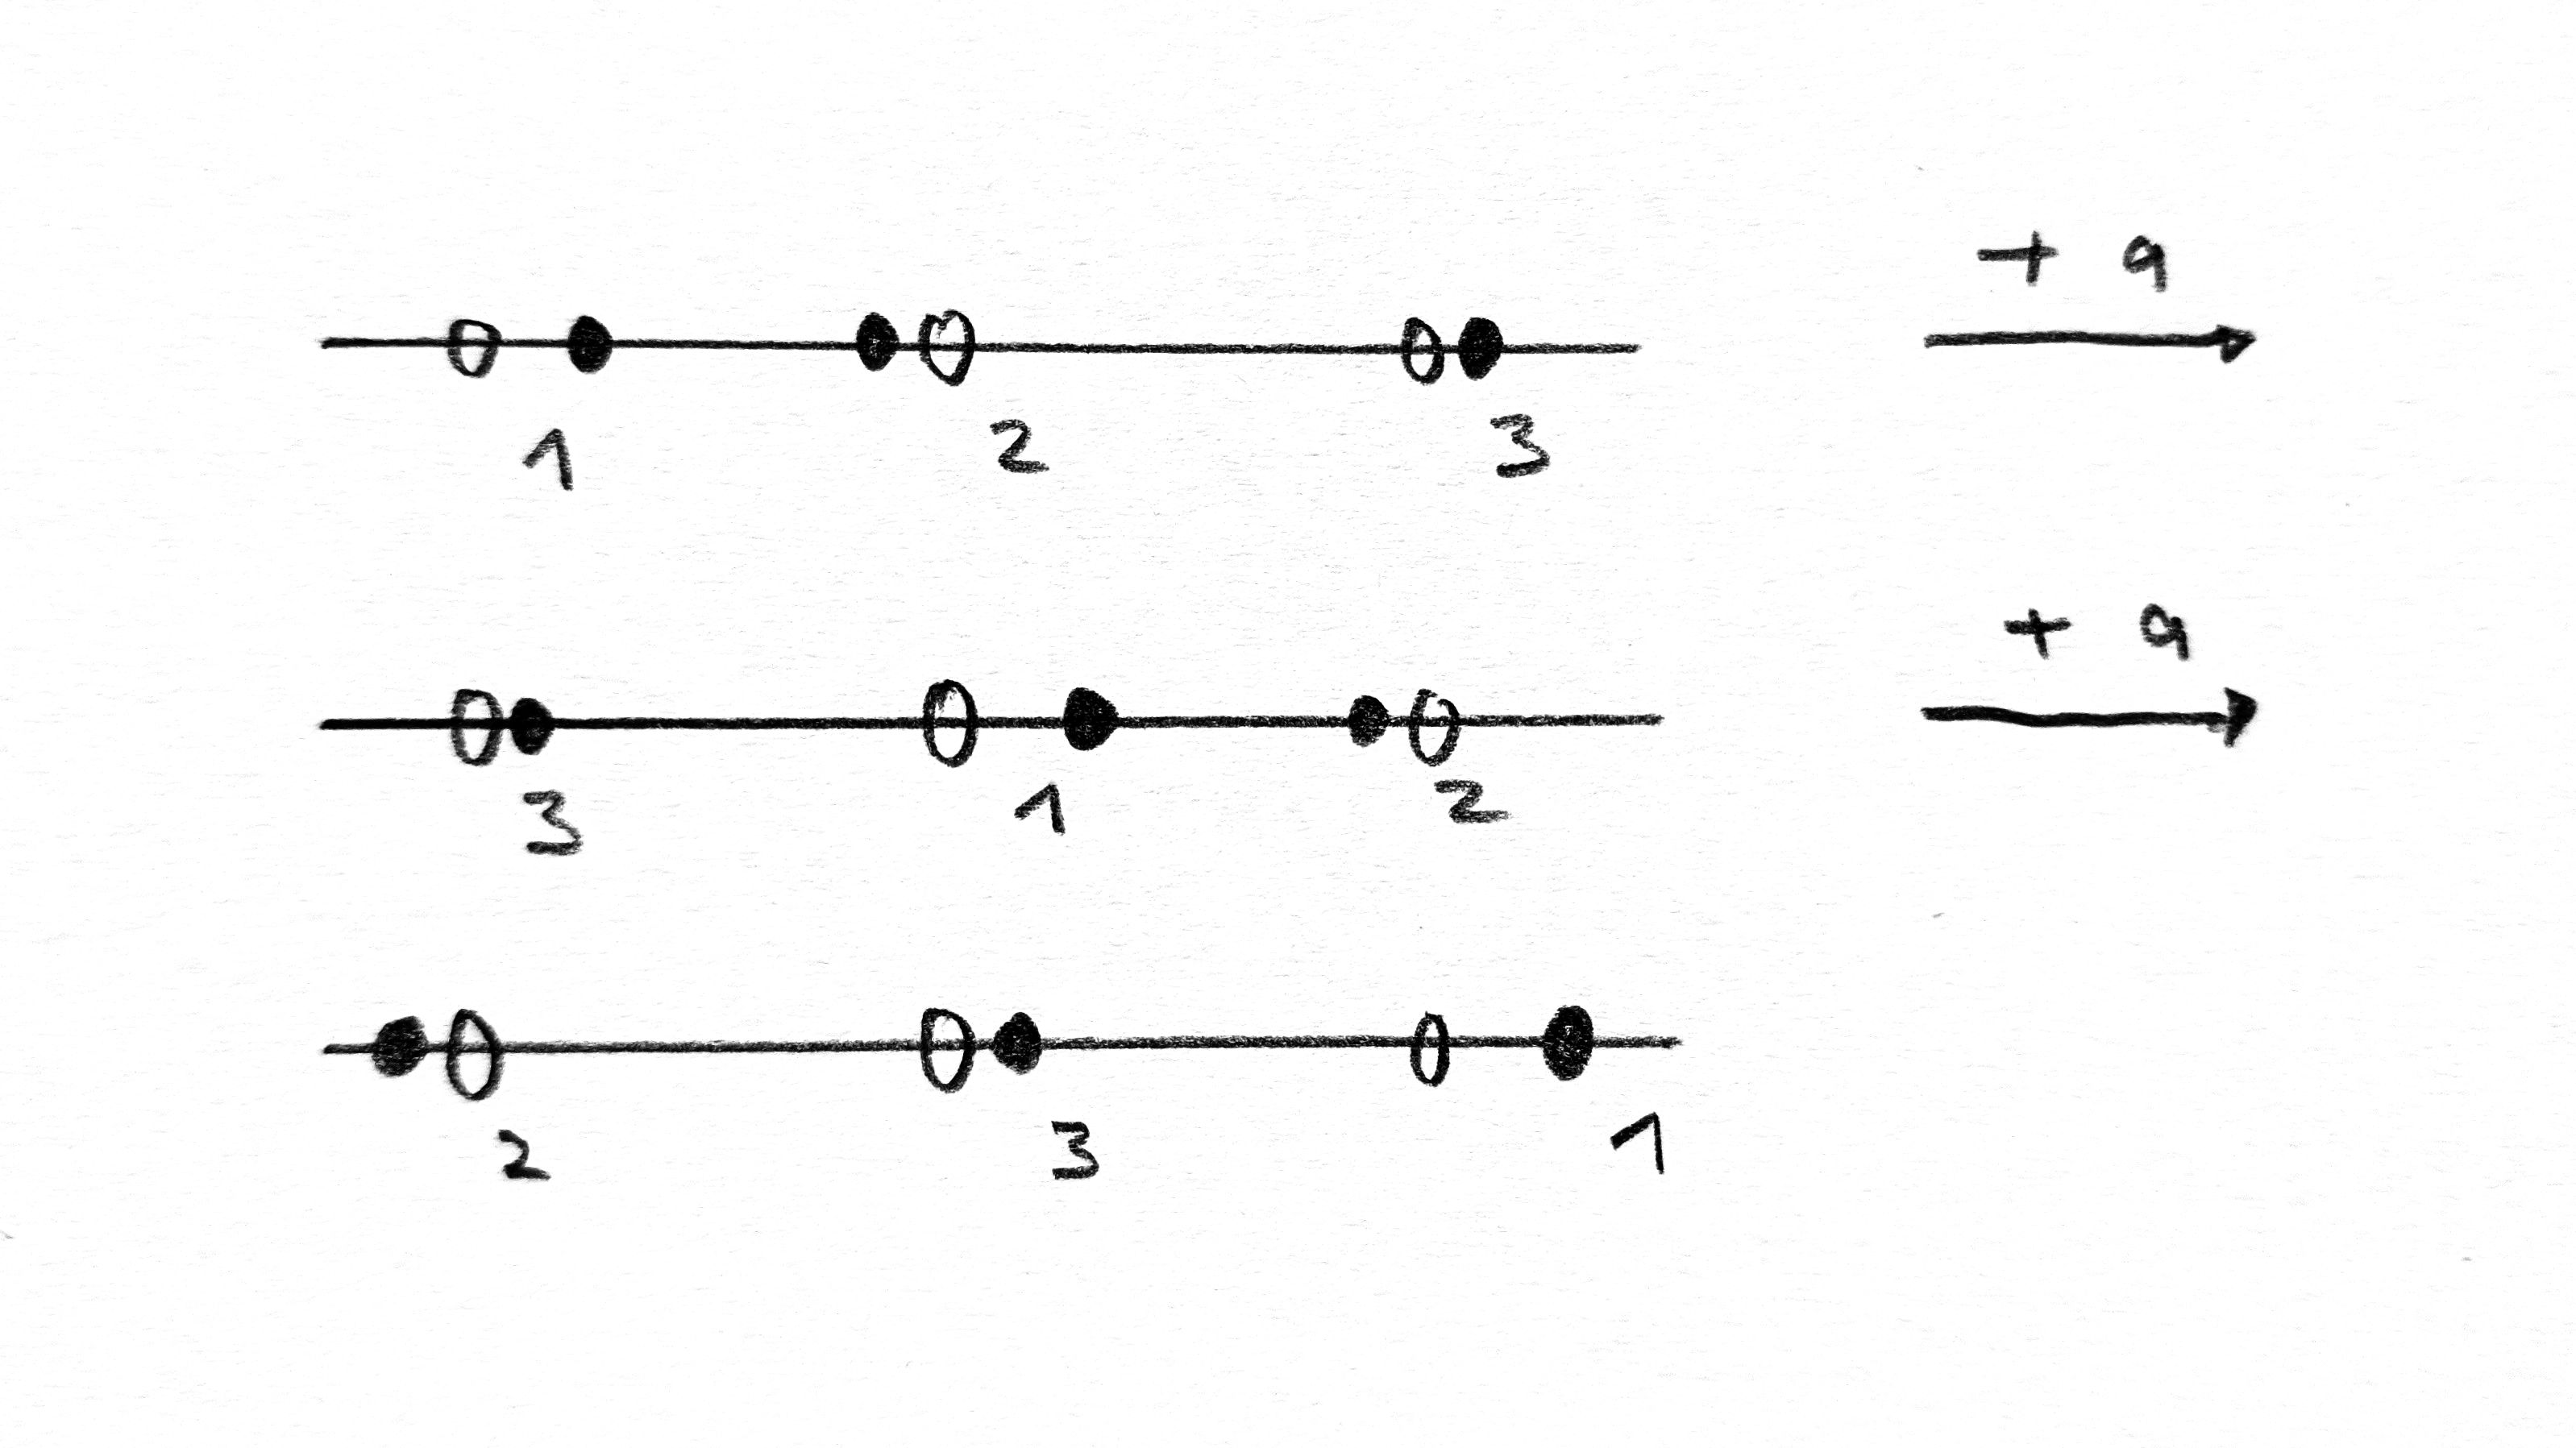
\includegraphics[width=.68\textwidth]{./sketches/permutation1.jpg}
	\caption{A linear chain with three atoms (bullets) displaced from their equilibrium position (open circels). With periodic boundary conditions, the consecutive translation by a lattice vector $a$ induces a permutation of the atoms,~i.\,e.,~$(1, 2 , 3) \to (3, 1, 2) \to (2, 3, 1)$.}
	\label{fig:translation.permutation}
\end{figure}

We can draw two important conclusions from Eq.\,\eqref{eq:translation.permutation} and \eqref{eq:inv.V}. First, the existence of the map $P_{\bf L}$ enables us to write every atomic coordinate ${\bf R}_I$ as
\begin{align}
	{\bf R}_I \equiv {\bf R}_{i {\bf L}} 
		= {\bf R}^0_i + {\bf U}_{i {\bf L}} + {\bf L}~,
	\label{eq:R_iL}
\end{align}
where ${\bf R}^0_i$ labels the position of an equivalent reference atom in the unit cell, ${\bf U}_{i {\bf L}}$ is the displacement of the atom from its equilibrium position, and $\bf L$ is a Bravais vector as before.
We can therefore split the index $I$ into a tuple $I = (i, {\bf L})$,~i.\,e.,~unit cell and lattice point labels.

Second, the harmonic force constants $\Phi_{I \alpha, J \beta}$ can be written as $\Phi_{i {\bf L} \alpha, j {\bf K} \beta}$~, where $\bf L$ and $\b K$ are the Bravais vectors belonging to $I$ and $J$, respectively. From the translational invariance of the potential, Eq.\,\eqref{eq:inv.V}, we see that the force constants have to fulfill
\begin{align}
	\Phi_{i {\bf L} + \b M \alpha, j {\bf K} + \b M \beta} 
		= \Phi_{i {\bf L} \alpha, j {\bf K} \beta}~,
	\label{eq:fc.sym.1}
\end{align}
where $\b M$ again denotes an arbitrary Bravais vector. Using this translational invariance, we can Fourier transform the dynamical matrix defined in Eq.\,\eqref{eq:D},
\begin{align}
	{\rm D}_{i \alpha, j \beta} (\b q) 
		= \sum_{\b L} {\rm e}^{- \im \b q \cdot \b L} {\rm D}_{i \b 0 \alpha, j \b L \beta}
	\label{eq:D(q)}
\end{align}
where we restrict the values of $\b q$ to reside in the first Brillouin zone, thereby transforming the $3N \times 3N$ matrix ${\rm D}_{IJ}$ to one $3n \times 3n$ matrix ${\rm D}_{ij} (\bf q)$ for each~$\b q$, where $n$ is the number of atoms in the primitive unit cell.

\subsubsection{Cyclic Boundary Conditions and Supercell Approximation}
In the previous section, we did not specify the system beyond requiring periodic boundary conditions, and implicitly assumed an infinite crystal in the limit $N \to \infty$ without boundaries. In practice we introduce Born-von Karman cyclic boundary conditions~\cite{born2013atomtheorie}, as already done in Sec.\,\ref{sec:theory.periodic.1} for the description of electronic states, but reintroduce them here in a slightly more general fashion.

We define the boundary conditions for the nuclear problem such that
\begin{align}
	\b R_I + S^i \b A_i = \b R_I \quad\text{for}\quad S^i \in \mathds{Z}~,
	\label{eq:sc.1}
\end{align}
where each ${\bf A}_i$ is a linear combination of the primitive basis vectors $\set{{\bf a}_i}$,
\begin{align}
{\bf A}_i = {\rm M}_{ij}^{\rm sc} {\bf a}_j\quad\text{with } {\rm M}_{ij}^{\rm sc} \in \mathds Z~,
\end{align}
and $\rm M^{\rm sc}$ is a non-singular matrix with integer elements. The space spanned by the $\set{{\bf A}_i}$ is parallelepiped of volume $V_{\rm sc} = N_{\rm sc} \, {\bf a}_1 \cdot ({\bf a}_2 \times {\bf a}_3)$, where $N_{\rm sc} = \det {\rm M}^{\rm sc}$ is the number of unit cells that fit into the enlarged cell, and $V_{\rm uc} = {\bf a}_1 \cdot ({\bf a}_2 \times {\bf a}_3)$ is the unit cell volume. This cell is therefore called \emph{supercell} and we define it such that its midpoint is located at the origin,~i.\,e.,~
\begin{align}
	\mathds V_{\rm sc}
		&= \set{{\bf X} = X^i {\bf A}_i : X^i \in {[-0.5, 0.5)_{\mathds R}}}~.
	\label{eq:supercell}
\end{align}
We therefore denote the matrix ${\rm M}^{\rm sc}$ as the \emph{supercell matrix}.
The vectors \mbox{$\b S = S^i \b A_i$} are the equivalent of the Bravais vectors $\b L$ in a superlattice described by $\set{ \b A_i }$ instead of $\set{ \b a_i}$.
The ideal, infinite crystal is obtained in the limit $N_{\rm sc} \rightarrow \infty$.
From Eq.\,\eqref{eq:sc.1} we see that the force constants become periodic functions in the superlattice,
\begin{align}
	\Phi_{i {\bf L} \alpha, j {\bf K} + \b S \beta} 
		= \Phi_{i {\bf L} \alpha, j {\bf K} \beta} \quad\text{for all}\quad \b S = S^i \b A_i~,
	\label{eq:fc.sym.2}
\end{align}
so that the dynamical matrix in Eq.\,\eqref{eq:D(q)} can be written as a sum over lattice points that are contained in the supercell only,
%\begin{align}
%	{\rm D}_{i \alpha, j \beta} (\b q) 
%		&= \sum_{\b L \in \mathds V_{\rm sc}} 
%			\left( 
%				{\rm e}^{- \im \b q \cdot \b L} {\rm D}_{i \b 0 \alpha, j \b L \beta}
%			+ \sum_{\b S \neq \b 0} {\rm e}^{- \im \b q \cdot (\b L + \b S)} {\rm D}_{i \b 0 \alpha, j \b L \beta}
%			\right)~.
%	\label{eq:D^S(q).1}
%\end{align}
\begin{align}
	{\rm D}_{i \alpha, j \beta} (\b q_{\bf m}) 	
		&= %\frac{N}{N_{\rm sc}} 
	\sum_{\b L \in \mathds V_{\rm sc}} {\rm e}^{- \im \b q_{\bf m} \cdot \b L} {\rm D}_{i \b 0 \alpha, j \b L \beta}~.
	\label{eq:D^S(q).2}
\end{align}
for $\b q_{\b m}$ that fulfill
\begin{align}
	{\bf q_{\b m}} \cdot {\bf A}_i	= 2 \pi m_i \quad\text{with}\quad m_i \in \mathds Z~.
	\label{eq:q.commensurate}
\end{align}
%the summands in the second sum of Eq.\,\eqref{eq:D^S(q).1} interfere constructively and yield a factor $\sum_{\b S}' = N / N_{\rm sc} - 1$. For all other $\b q$, the entire summand becomes negligible in the limit $N \to \infty$ when normalized to the supercell volume.
The $\b q_{\b m}$ that fulfill Eq.\,\eqref{eq:q.commensurate} are called \emph{commensurate} $\b q$-points, as they represent wave numbers that fit into the supercell.
In total there are $N_{\rm sc}$ non-equivalent values of $\bf q_{\b m}$ labelled by ${\bf m} = (m_1, m_2, m_3)$ that can be expressed in terms of the lattice vectors of the reciprocal supercell,
\begin{align}
{\bf B}^i 
= 2 \pi \varepsilon^{ijk} \frac{{\bf A}_j \times {\bf A}_k}{{\bf A}_1 \cdot ({\bf A}_2 \times {\bf A}_3)} ~,
%\label{eq:dft.Bloch.bi}
\end{align}
where $\varepsilon^{ijk}$ denotes the Levi-Civita symbol enforcing the correct ordering of $ijk$. The complete set of $\bf q$-values is
\begin{align}
{\bf q}_{\bf m} 
= \sum_{i=1}^3 m_i {\bf B}^i~,
\label{eq:q_m}
\end{align}
with $m_i \in \mathds Z$ such that $\b q_{\bf m}$ is an element of the first Brillouin zone of the direct lattice.
%For the set of commensurate $\b q$-points, the dynamical matrix is therefore given by
%\begin{align}
%{\rm D}_{i \alpha, j \beta} (\b q_{\bf m}) 	
%	&= %\frac{N}{N_{\rm sc}} 
%	\sum_{\b L \in \mathds V_{\rm sc}} {\rm e}^{- \im \b q_{\bf m} \cdot \b L} {\rm D}_{i \b 0 \alpha, j \b L \beta}~.
%	\label{eq:D^S(q).2}
%\end{align}


\subsubsection{Interpolation to non-commensurate q-points}
The definition of the dynamical matrix in Eq.\,\eqref{eq:D^S(q).2} was formulated for commensurate $\b q$-points $\set{\b q_{\b m}}$,~i.\,e.,~those given in terms of Eq.\,\eqref{eq:q_m}. Evaluating this expression at a non-commensurate value of $\b q$ will, in general, yield a non-hermitian matrix which cannot be used to extract physically sound information about the system. To obtain an \emph{approximated} dynamical matrix at any other, non-commensurate value of $\b q$ within the Brillouin zone, we define an \emph{extended supercell}, 
\begin{align}
	\mathds V_{\rm sc}^{\rm ext}
		&= \set{{\bf X} = X^i {\bf A}_i : X^i \in {[-0.5, 0.5 \boldsymbol{]}_{\mathds R}}}~,
	\label{eq:supercell.extended}
\end{align}
which also contains the lattice points at the positive boundary of the supercell as depicted by open circles in Fig.\,\ref{fig:sketch_supercells}.
\begin{figure}[t]
	\centering
	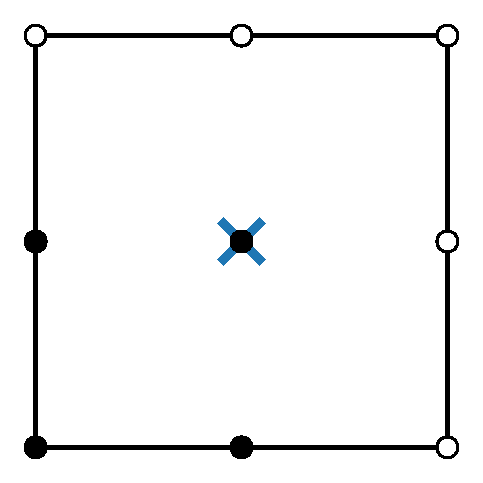
\includegraphics[width=.32\textwidth]{./sketches/2_sc.pdf}
	\hfill
	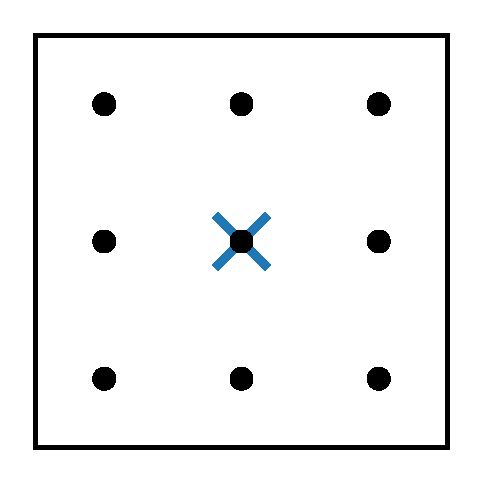
\includegraphics[width=.32\textwidth]{./sketches/3_sc.pdf}
	\hfill
	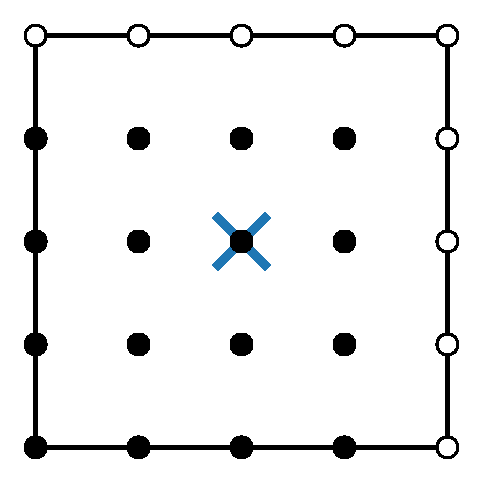
\includegraphics[width=.32\textwidth]{./sketches/4_sc.pdf}
	\caption{Depiction of square supercells with lattice points in the range $[-0.5 A, 0.5 A)$ (bullets $\bullet$), and extended lattice points at the supercell boundary (empty bullets $\circ$), where $A$ is the edge length of the supercell. Blue arrows denote the unit cell vectors, black arrows denote the supercell vectors.}
	\label{fig:sketch_supercells}
\end{figure}
These lattice points are included in the Fourier series with an appropriate weight $w_{\b L}$ that accounts for double counting of lattice points that are separated by a linear combination of supercell lattice vectors~\cite{Parlinski1997}. Furthermore, we use a minimal image convention (MIC) between the atoms $(i, \b 0)$ and $(j, \b L)$,~i.\,e.,~for each pair we use an equivalent lattice point $\b L'$ within the extended supercell which depends on $(i, j, \b L)$ such that
\begin{align}
	- \b R_{i \b 0 } + \b R_{j \b 0} + \b L' \in V_{\rm sc}^{\rm ext}~.
	\label{eq:L'}
\end{align}
In total we define
\begin{align}
	{\rm D}_{i \alpha, j \beta} (\b q) 	
		&= %\frac{N}{N_{\rm sc}} 
		\sum_{\b L \in \mathds V_{\rm sc}^{\rm ext}} 
			w_{\b L}
		{\rm e}^{- \im \b q \cdot \b L'} {\rm D}_{i \b 0 \alpha, j \b L \beta}~.
	\label{eq:D_Parlinski}
\end{align}
We note that the dynamical matrix elements defined by Eq.\,\eqref{eq:D_Parlinski} differ from the ones found in Ref.~\cite{Parlinski1997} by a phase factor ${\rm e}^{\im \b q \cdot (\b R_i^0 - \b R_j^0)}$, which is typical when the discussion is performed from a lattice-wave ansatz to solve the equations of motion~\cite[p. 298]{BornHuang}.

For each $\b q$, ${\rm D} (\b q)$ is a hermitian $3n \times 3n$ matrix in the indices $(i \alpha, j \beta)$ and will therefore yield $3n$ real eigenvalues and $3n$ complex, orthogonal eigenvectors, which denote in accordance with Eq.\,\eqref{eq:sum_D_IJ}
\begin{align}
\sum_{j \beta} {\rm D}_{i \alpha, j \beta} (\b q) e_{j \beta} (\b q , b)
= \omega^2 \, (\b q, b) e_{i \alpha} (\b q , b)~,
\label{eq:D_ij(q)w}
\end{align}
where the \emph{band index} $b$ is used to discern the $3n$ \emph{branches} at each $\b q$. Using the combined index $s = (\b q, b)$, the notation becomes similar to the non-periodic case with $3N_{\rm sc} N_{\rm uc}$ degrees of freedom, only that the eigenvectors $\b e_{s = (\b q, n)}$ can be complex valued instead of strictly real.
\REM{This is Born conventions. Togo and Parlinski use extra phase factor ${\rm e}^{\im \b q \cdot (\b R_i^0 - \b R_j^0)}$ that alters the eigenvectors but not the frequencies.}

\subsubsection{Ledermann's Theorem}

%As we will be interested in the eigenvalues and eigenvectors of the dynamical matrices $\rm D ({\b q})$, the prefactor $N/N_{\rm sc}$ can be neglected in the following.

\REM{for $\b q = \b q_{\b m}$ D is exact up to boundary effects (?!), nevertheless one can interpolate -> Fourier interpolation}
\REM{Alternative: Use effective cutoff of $\Phi$}
\REM{Effective cutoff -> effect on spectrum, Maradudin, Ledermann}

% Equation~\eqref{eq:D^S(q).2} will in general not be hermitian in $(i \alpha, j \beta)$

\subsubsection{Finite Differences}
The force constants can be obtained from first-order derivatives of the potential-energy surface,~i.\,e.,~the forces, by rewriting the second derivative in terms of a finite difference expression,
\begin{align}
	\Phi_{I \alpha, J \beta}
		= \left.\frac{\partial^{2} \mathcal{V}(\mathbf{R})}{\partial R_{I}^{\alpha} \partial R_{J}^{\beta}}\right|_{\mathbf{R}^{0}}
		= - \frac{\partial}{\partial R_I^\alpha} F_{J, \beta}
		= - \lim_{\epsilon \to 0}
			\frac{F_{J, \beta} (\set{\b R': R^{\prime \beta}_I = R^{\beta}_I + \epsilon )}}{\epsilon}
		~.
\label{eq:FC2_finite}
\end{align}
In practice, atom $J$ is displaced by a small but finite displacement $\epsilon$ in the direction $\beta$, and the force on all other atoms is recorded. By performing the displacement in all $3N$ degrees of freedom, the $3N \times 3N$ forces can be arranges in a matrix $F_{[3N \times 3N]}$, and the displacements can be arranged in a matrix $U_{[3N \times 3N]} = \epsilon \mathds 1_{[3N \times 3N]}$. The $3N \times 3N$ force-constants matrix $\Phi$ is obtained by the trivial matrix inversion
\begin{align}
F &= - H U = - \epsilon \Phi \mathds 1\\
\implies
\Phi &= - \frac{1}{\epsilon} F \mathds 1~.
\end{align}
%\begin{align}
%	F &= - H U \\
%	\implies
%	H &= - U^{+} F \\
%	F &= \begin{pmatrix} \b F_1, & \cdots, & \b F_{3N} \end{pmatrix}
%\end{align}
If $M > 3N$ displacements are used,~e.\,g.,~because positive and negative displacements $\pm \epsilon$ are used, the force constants can be obtained by solving an overdetermined linear equation of the kind
\begin{align}
	F_{[3N \times M]} &= - \Phi_{[3N \times 3N]} U_{[3N \times M]} \\
	\implies
	\Phi &= - U^{+} F~,
%	F &= \begin{pmatrix} \b F_1, & \cdots, & \b F_{3N} \end{pmatrix}
\end{align}
where $U^{+}$ denotes the Moore-Penrose pseudo inverse of the displacement matrix $U$~\CITE{pseudoinverse}.
\CITE{Parlinski, Togo}

In practice, the number of required force calculations can be reduced by considering the spacegroup symmetry of the crystal. This can be achieved in two ways: First, the symmetry can be used to identify the set of inequivalent displacements from which all other forces can be reconstructed. Second, the symmetry can be used to reduce the forceconstant matrix to an irreducible basis.

\REM{Symmetry: 2 ways: i) construct full $F$ from a reduced set of displacements, ii) reduce $H$ to reduces/irreducible representation like original Parlinski article.}

\subsection{Harmonic Sampling}

\subsection{Molecular Dynamics}
The classical limit of the nuclear Schr\"odinger equation~\eqref{eq:BOSE} is usually performed by writing the nuclear wavefunction $\chi_s ({\bf R}, t)$ in terms of a real amplitude $A_s({\bf R}, t)$ and a \emph{classical action function} $S_s({\bf R}, t)$~\cite{Dirac1981,Landau2013,Marx2009}
\begin{align}
	\chi_s({\bf R}, t) = A_s({\bf R}, t) \, {\rm e}^{\frac{\im}{\hbar} S_s({\bf R}, t)}~.
	\label{eq:class.1}
\end{align}
The Schr\"odinger equation then yields a set of differential equations for $A_s$ and $S_s$ that, in the limit $\hbar \to 0$, go over to a \emph{Hamilton-Jacobi} equation for $S_s$,~i.\,e.,~
\begin{align}
  \frac{\partial S_s}{\partial t} + \mathcal H \left({\bf R}, {\bf P}\right)
  = 0~,
  \label{eq:HamiltonJacobi}
\end{align}
where ${\bf P} = ({\bf P}_1, \ldots) \equiv ({\bf \nabla}_1 S_s, \ldots)$ denotes the conjugate momenta and $\mathcal H$ is the \emph{classical} Hamilton function corresponding the to the operator in Eq.\,\eqref{eq:BOSE}, from which the equations of motion for the nuclei can be obtained:
\begin{align}
  \dot{{\bf P}}_I 
    = -\frac{\partial \mathcal H}{\partial {\bf R}_I}
    \quad\implies\quad M_I \ddot{\bf R}_I
    = -\frac{\partial \mathcal V}{\partial {\bf R}_I}~.
    % \equiv - {\bf F}_I~.
\end{align}
The negative gradient of the Born-Oppenheimer potential, 
$-\partial \mathcal V / \partial {\bf R}_I$ is the force ${\bf F}_I$ acting on atom $I$ which can be obtained via the Hellmann-Feynmann theorem,~cf.~Sec.\,\ref{sec:HellmannFeynman}.

An alternative viewpoint that is more instructive can be taken by invoking the \emph{Ehrenfest theorem}~\cite{Ehrenfest1927,Basdevant2007}. The statement is that
\begin{align}
  \frac{\d}{\d t} \left\langle {\bf P}_I \right\rangle_{\chi_s}
    = \left\langle
      - \frac{\partial \mathcal{V}}{\partial {\bf R}_I}
    \right\rangle_{\chi_s}~,
  \label{eq:ehrenfest.de1}
\end{align}
where $\langle \cdot \rangle_{\chi_s}$ denotes an expectation value taken with respect to the state $\chi_s$. This expression differs only slightly from the classical counterpart, which would read
\begin{align}
\frac{\d}{\d t} \left\langle {\bf P}_I \right\rangle
= \left.
- \frac{\partial \mathcal{V}}{\partial {\bf R}_I}
\right\vert_{{\bf R} = \langle {\bf R} \rangle}~.
\label{eq:ehrenfest.de2}
\end{align}
The difference comes from the fact that, in general,
\begin{align}
  \delta f  \equiv 
  f \bm ( \langle x \rangle \bm{)} 
  - 
  \bm{\langle} f (x) \bm{\rangle}
  \neq 0
  ~,
  \label{eq:ehrenfest.delta1}
\end{align}
where $x = {\bf R}_I$ denotes the space coordinate for notional simplicity, $f$ is some function of the observable $x$, and $\delta f$ measures the difference between the classical and the quantum expectation value. Ehrenfest's argument is that this difference becomes negligible when the state is sufficiently peaked around some value $x_0$. Expanding $f$ around the expectation value of $x$, $x_0 \equiv \langle x \rangle$, we have
\begin{align}
  f(x) = f \bm ( \langle x \rangle \bm{)}  
    + (x - \langle x \rangle) \, f' \bm ( \langle x \rangle \bm{)}
    + \frac{1}{2} (x - \langle x \rangle)^2 \, f'' \bm ( \langle x \rangle \bm{)}
    + \cdots~.
  \label{eq:ehrenfest.f2}
\end{align}
It follows that the $f'$ term vanishes when the expectation value is taken, and
\begin{align}
\langle f(x) \rangle 
  = f \bm ( \langle x \rangle \bm{)}  
    + \frac{1}{2} \Delta x^2 f'' \bm ( \langle x \rangle \bm{)}
    + \cdots~,
\label{eq:ehrenfest.f3}
\end{align}
where $\Delta x^2 = \bm{\langle} (x - \langle x \rangle)^2 \bm{\rangle}$ measures the variance of the underlying distribution,~i.\,e.~the width of the wavepacket. The relative error between the classical and quantum expectation value is readily computed to be
\begin{align}
  \left\lvert \frac{\delta f}{f \bm ( \langle x \rangle \bm{)}} \right\rvert
  = \frac{1}{2} \Delta x^2 \left\lvert \frac{f'' \bm ( \langle x \rangle \bm{)}}{f \bm ( \langle x \rangle \bm{)}} \right\rvert
+ \mathcal{O}(\Delta x^3)~.
  \label{eq:ehrenfest.delta2}
\end{align}
This estimation holds in general for any observable $f$.
By crudely estimating the dimension of the wavepacket in terms of the thermal de Broglie-wavelength, we find
\begin{align}
  \Delta x^2 
    \sim \left( \frac{h}{P} \right)^2
    \sim \frac{h^2}{MT}~,
  \label{eq:ehrenfest:dimension}
\end{align}
which gives support to the intuitive assumption that we can expect the classical limit to work better the heavier the atoms and the higher the temperature.
Let us now set $f(x) \hat = -\partial \mathcal V / \partial {\bf R}_I$, then another important conclusion can be drawn from Eq.\,\eqref{eq:ehrenfest.delta2}: For a harmonic potential $\mathcal V ({\bf R}) = \mathcal V^{(2)} ({\bf R})$, where derivatives higher than second order vanish, the classical and quantum mechanical expectation values \emph{always coincide}. The quantum mechanical expectation value of position will therefore evolve in the same time-periodic fashion as a classical particle in a harmonic well.

\REM{this approach can only be validated by computing observables and compare the results. One can safely say that this approach has been used successfully in a plethora of studies, while additional care must be taken at low temperature and/or systems with light atoms, especially hydrogen-bonded systems~\CITE{MD-Review?,MarklandCeriotti,Litman,pHexperiment}.}

\subsubsection{Thermodynamic Ensembles and Thermostats}
\subsubsection{Finite Temperature Equations of State and Lattice Expansion}
\subsubsection{Mode Projection}
\subsubsection{Approximative Anharmonic Methods}

\subsection{Heat Transport}
\subsubsection{Fluctuation Dissipation Theorem}
\subsubsection{Green and Kubo}
\subsubsection{Ab initio Virial Heat Flux}
\subsubsection{Ab initio Green Kubo}

\chapter{Heat Transport}
\epigraph{\singlespacing \it ``It seems there is no problem in modern physics for which there are on record as many false starts, and as many theories which overlook some essential feature, as in the problem of the thermal conductivity of [electrically] non-conducting crystals.''}{R.~Peierls, 1960}


Conductive heat transport is the phenomenon of vibrational energy traversing a material when a temperature gradient is applied. As first described by Joseph Fourier in the early 19th century~\cite{Fourier1878}, the heat flux $\b J$ resulting from a stationary temperature gradient $\nabla T$ is directly proportional to this gradient. The proportionality constant is second-rank tensor denoted by $\kappa$ and called the \emph{thermal conductivity}. The defining equation,
\begin{align}
  \b J = - \kappa \nabla T~,
  \label{eq:Fourier}
\end{align}
is called \emph{Fourier's law}. The sign convention is such that the heat flux points ``from hot to cold''. The regime where Eq.\,\eqref{eq:Fourier} is valid is called the \emph{diffusive} regime, as it holds when the temperature gradient is small on microscopic scale, and the sample size is big enough so that boundary effects are negligible~\cite{Kapitza1941a,Antidormi2020}.

It is evident from Eq.\,\eqref{eq:Fourier} that the thermal conductivity $\kappa$ is an explicitly non-equilibrium quantity. As such, it can however be related to equilibrium fluctuations by means of the \emph{fluctuation-dissipation theorem}~\cite{Einstein1905a,Nyquist1928,Callen1951,Kubo1957a}, resulting in the famous Green-Kubo formula~\cite{Green1952,Kubo1957b},
\begin{align}
  \kappa^{\alpha \beta} = \frac{V}{k_{\rm B} T^2} \int_{0}^{\infty} \d t ~
    \braket{J^\alpha (t) J^\beta(0)}_{\rm eq}~.
  \label{eq:GreenKubo}
\end{align}
This formula relates the temporal fluctuations of the macroscopic heat flux $\b J (t)$ as given by an equilibrium ensemble average of the autocorrelation function, $\braket{J^\alpha (t) J^\beta(0)}_{\rm eq}$, to the associated transport coefficient $\kappa$. It is however \emph{a priori} unclear how a microscopic description of the appearing quantities can be obtained. To tackle this question in full, we first show how the Kubo formula emerges in the framework of linear response theory. We then present how a microscopic description of heat in terms of a thermal energy density and an associated, locally conserved current follows, before reviewing the necessary steps to define an \emph{ab initio} heat flux~\cite{Carbogno2016}.

\section{Linear Response Theory}
The aim of linear response theory is to compute the expected value of a phase-space observable $B$ in presence of an external perturbation driving the system out of equilibrium. The ensemble is characterized by a \emph{distribution function} $f(\Gamma, t)$, where $\Gamma = \set{\b R, \b P}$ is a shorthand for a point in phase space. The expectation value of $B$ is given by
\begin{align}
  \braket{B (t)}_{f}
    = \int \d \Gamma ~ B (\Gamma) f(\Gamma, t)~,
  \label{eq:lr.B.1}
\end{align}
and we assume without loss of generality that its equilibrium value vanishes,
\begin{align}
\braket{B (t)}_{f^0}
= \int \d \Gamma ~ B (\Gamma) f^0(\Gamma) = 0~,
\label{eq:lr.B0}
\end{align}
where $f^0 (\Gamma)$ is the distribution function of the unperturbed system in thermal equilibrium. In order to calculate Eq.\,\eqref{eq:lr.B.1} in a non-equilibrium situation, we start by defining the Hamiltonian describing the equilibrium dynamics, $H^0$, which we take to be given by the many-body Hamiltonian
\begin{align}
  H^0 (\Gamma) 
    %= H^0(\set{\b R, \b P})
    = \sum_I \frac{\b P_I^2}{2 M_I} + V (\b R)~.
  \label{eq:lr.H0}
\end{align}
The canonical distribution function for the unperturbed system reads
\begin{align}
f^0 (\Gamma) 
= \frac{1}{\mathcal{Z}^0} {\rm e}^{- \beta H^0 (\Gamma)}~,
\label{eq:lr.f0}
\end{align}
where the partition sum $\mathcal{Z}_0$ normalizes the phase-space integral, \mbox{$\int \d \Gamma f^0 (\Gamma) = 1$}.
In the next step, we write the full Hamiltonian as
\begin{align}
  H (\Gamma, t)
   = H^0 (\Gamma) + \lambda H' (\Gamma, t)~,
  \label{eq:lr.H}
\end{align}
where the perturbation is given by some yet unspecified phase-space function $H' (\Gamma, t)$ with explicit time dependence, and $\lambda = 1$ is a bookkeeping parameter that we introduce to count the order in the perturbation.
We write the distribution function in presence of the perturbation as
\begin{align}
  f (\Gamma, t) = f^0(\Gamma) + \lambda \Delta f (\Gamma, t)~,
  \label{eq:lr.f}
\end{align}
where $\Delta f$ is the perturbation in the distribution generated by $H'$. Using that $f^0$ carries no explicit time dependence, the Liouville equation for $\Delta f$ reads
\begin{align}
  \lambda \frac{\d \Delta f}{\d t}
    &= \set{H, f} \nonumber \\
    &= \lambda \set{H^0, \Delta f} 
      + \lambda \set{H', f^0}
      + \mathcal{O}(\lambda^2)~,
  \label{eq:lr.df.1} \\
  \implies
    \frac{\d \Delta f}{\d t}
      &\approx \set{H^0 , \Delta f} + \set{H' (t), f^0}
  \label{eq:lr.df.2}
\end{align}
where $\set{\cdot , \cdot}$ denotes the Poisson bracket
%\footnote{
%  The Poisson bracket for a system of particles with $3N$ positions $q_i \equiv R_I^\alpha$ and conjugate momenta $p_i \equiv P_I^\alpha$ reads
%  $$
%  \set{A, B} = \sum_{i}
%  \frac{\partial A}{\partial q_i} \frac{\partial B}{\partial p_i}
%  - \frac{\partial A}{\partial p_i} \frac{\partial B}{\partial q_i}~.
%  $$
%  }, 
and in Eq.\,\eqref{eq:lr.df.2} we only keep the terms to linear order in the perturbation.
The solution to this differential equation is found to be\footnote{The solution is given in appendix \ref{app:lr.f}.}~\cite{Kubo1957a}
\begin{align}
  \Delta f (t) 
    = \int_{-\infty}^t {\rm e}^{-\im L^0 (t - t')} \set{H' (t'), f^0}~\d t'~,
  \label{eq:lr.df(t)}
\end{align}
where $\exp (\im L^0 t)$ propagates a phase-space point $\Gamma$ by a time $t$ according to the equations of motion following from $H^0$.
By splitting the interaction Hamiltonian $H'(t)$ into an operator part $A(\Gamma)$ and an explicitly time dependent force function $F(t)$,
\begin{align}
  H' (t)=AF(t)~,
\end{align}
this expression can be simplified in the canonical ensemble by using that \mbox{$\partial f^0 / \partial H^0 = -\beta f^0$}, which leads to
\begin{align*}
  \set{A, f^0}
%    &= \sum_i \frac{\partial A}{\partial q_i} \frac{\partial f^0}{\partial p_i}
%    - \frac{\partial A}{\partial p_i} \frac{\partial f^0}{\partial q_i} \\
%    &= \sum_i \frac{\partial A}{\partial q_i} \frac{\partial f^0}{\partial H^0} \frac{\partial H^0}{\partial p_i}
%    - \frac{\partial A}{\partial p_i} \frac{\partial f^0}{\partial H^0} \frac{\partial H^0}{\partial q_i} \\
%    &= -\beta f^0 \sum_i
%      \left( \frac{\partial A}{\partial p_i} \dot{q}_i +  \frac{\partial A}{\partial q_i} \dot{p}_i \right) \\
    &= -\beta f^0 \, \frac{\d A}{\d t}~.
\end{align*}
%where in the second step Hamilton's equations of motion have been used.

We are now in the position to formulate the expected response of a phase space observable $B$ to linear order in a perturbation described by the Hamiltonian $H'(t) = A F(t)$,~i.\,e.,~
\begin{align}
\braket{B (t)}_f
    &= \int \d \Gamma ~  B (\Gamma) \Delta f (\Gamma, t) \\
    &= - \beta \int_{-\infty}^t 
      \int \d \Gamma ~  
       B (\Gamma) \, {\rm e}^{-\im L^0 (\Gamma) (t - t')} \dot{A}(\Gamma)
       f^0(\Gamma) F(t') ~ \d t' \\
    &= - \beta \int_{-\infty}^t 
      \braket{B(t) \dot{A}(t')}_{f^0} F(t') ~ \d t'~,
  \label{eq:lr.dB}
\end{align}
where it was used that $a(t) = {\rm e}^{\im L^0 t} a(0) = a(0) {\rm e}^{-\im L^0 t}$~\cite[p.\,498]{Tuckerman}, and $\braket{\cdot}_{f^0}$ denotes a phase-space average with respect to the unperturbed canonical distribution function $f^0 (\Gamma)$. It is evident from this equation that the time propagation of the observables $\dot A$ and $B$ is generated by $L^0$ and therefore microcanonical with conserved energy. The phase-space average $\braket{\cdot}_{f^0}$ on the other hand corresponds to a canonical ensemble average with a defined inverse temperature $\beta$.

\subsection{Conserved densities and currents}
Macroscopic properties of matter are often \emph{extensive},~i.\,e.,~they scale with the system size, and can be described by a locally conserved \emph{density}. Taking the general property $A$ represented by the phase-space observable $A(\Gamma_t)$ evaluated at a time $t$ as an example, we define
\begin{align}
  A (\Gamma_t) = \int_V a (\b r, \Gamma_t) \, \d^3 r~,
  \label{eq:lr.A}
\end{align}
where $a(\b r, \Gamma_t)$ is the \emph{local density} associated with the observable $A$. The notation $\Gamma_t$ highlights that the quantity is implicitly time-dependent because the phase-space point $\Gamma$ evolves in time.
When no ambiguity arises, we can therefore just write $a (\b r, t)$.\footnote{
	Notation for phase-space functions $f (\Gamma)$:
	\begin{align*}
	f(t) &\equiv f(\Gamma (t)) \\
	\frac{\partial f}{\partial t} &= \frac{\d f (\Gamma (t))}{\d t} \equiv \dot{f}(t)
	\end{align*}
}
The locally conserved density fulfills a continuity equation
\begin{align}
  \partial_t \, a(\b r, t) = - \b \nabla \cdot \b j_a (\b r, t)~,
  \label{eq:lr.continuity.1}
\end{align}
where $\b j_a (\b r, t)$ is the associated current. From the local current, the macroscopic flux is obtained by spatially averaging over the system volume,
\begin{align}
  \b J (t)
    = \frac{1}{V} \int_V \d^3 r ~ \b j (\b r, t)~,
  \label{eq:lr.J(t)}
\end{align}
where the subscript $a$ was dropped for notational clarity.
Likewise we formulate a local version of the perturbing Hamiltonian \mbox{$H' = A (\Gamma) F(t)$} in the form
\begin{align}
	H' (\Gamma, t) = \int \d^3 r ~ a (\b r, \Gamma) v(\b r, t)~,
	\label{eq:lr.H'}
\end{align}
where $a(\b r, \Gamma)$ represents the density of interest as introduced above, and $v(\b r, t)$ is the local driving force coupling to the system via the density $a (\b r, \Gamma)$.

The local version of linear-response formula given in Eq.\,\eqref{eq:lr.dB} with \mbox{$\Delta B = B \equiv \b J$} ($\braket{\b J} = 0$) reads:
\begin{align}
j^\alpha (\b r , t) 
	& \equiv \braket{j^\alpha (\b r)}_{\Delta f (t)} \\
	&= - \beta \int_{-\infty}^{t} \d t' \int_V \d^3 r' ~ \braket{
			j^\alpha (\b r, \Gamma_t) \dot{a} (\b r', \Gamma_{t'})
		}_0 v (\b r', t')~.
	\label{eq:lr.ja.1}
\end{align}
The time derivative of the density can be eliminated by using the continuity equation~\eqref{eq:lr.continuity.1}, $\dot a = \partial'_\beta j^\beta$ where $\partial'_\beta = \partial/\partial r^{\prime \beta}$, and integrating by parts, so that
\begin{align}
j^\alpha (\b r , t) 
&= - \beta \int_{-\infty}^{t} \d t' \int_V \d^3 r' ~ \braket{
	j^\alpha (\b r, \Gamma_t) j^\beta (\b r', \Gamma_{t'})
}_0 \partial'_\beta v (\b r', t')~.
\label{eq:lr.ja.2}
\end{align}
If we now assume the external driving force $v (\b r, t)$ to be constant in time and homogeneously varying in space such that
\begin{align}
	\partial_\beta v (\b r, t) \equiv v_\beta~,
	\label{eq:lr.force}
\end{align}
and spatially average over Eq.\,\eqref{eq:lr.ja.2} with $\frac{1}{V} \int_V \d^3 r$, we arrive at
\begin{align}
	J^\alpha 
		&= -\beta V \int_{0}^{\infty} 
		\d t
		\braket{
		J^\alpha (\Gamma_t) J^\beta (\Gamma_{0})
	}_0 
	v_\beta~,
	\label{eq:lr.J}
\end{align}
where the stationarity in time was used to shift the lower bound of the integral to $t=0$.
This resembles the well-known macroscopic transport equation
\begin{align}
	J^\alpha =  L^{\alpha \beta} F_\beta~,
		\label{eq:lr.LF}
\end{align}
with
\begin{align}
	L^{\alpha \beta}
		= \frac{V}{k_{\rm B}} \int_{0}^{\infty} 
		\d t \braket{J^\alpha (\Gamma_t) J^\beta (\Gamma_{0})}_0 ~,
	\label{eq:lr.L}
\end{align}
and
\begin{align}
	F_\beta
		= - \frac{v_\beta}{T}~.
	\label{eq:lr.F}
\end{align}
Here, $J^\alpha$ is the macroscopic generalized current associated with the extensive property $A$, $F_\beta$ is the thermodynamic force, and $L^{\alpha \beta}$ is the associated conductance tensor~\cite{Onsager1931a,Baroni2020a}.

\subsection{Thermal Conductivity}
\label{sec:Thermal.Conductivity}
After this general exposition, let us now look at the example of the total energy of the system and its associated energy density,
\begin{align}
	E = \int_V \d^3 r ~ e(\b r)~.
	\label{eq:lr.E}
\end{align}
We are interested in the occuring flux in the presence of an inhomogeneous temperature, $T(\b r) = T + \Delta T(\b r)$, which couples linearly to the energy density  $e (\b r)$, so that\footnote{$E$ and $H(\Gamma)$ are related by $E = \braket{H}$. The same holds for the occurring densities $e(\b r)$ and $e (\b r, \Gamma)$.}
\begin{align}
	H (\Gamma) = \frac{1}{T} \int \d^3 r ~ T (\b r) e(\b r, \Gamma) 
		\equiv H^0 (\Gamma) + H' (\Gamma)~,
\end{align}
with
\begin{align}
	H' (\Gamma) = \frac{1}{T} \int \d^3 r ~ \Delta T (\b r) e(\b r, \Gamma)~.
	\label{eq:lr.Hp.temp}
\end{align}
With the previous assumption that $\Delta T(\b r)$ varies linearly in space, we find the thermodynamic force to be given by
\begin{align}
	v_\beta = \frac{1}{T} \partial_\beta T (\b r) 
		\stackrel{\eqref{eq:lr.F}}{\implies}
	F_\beta = - \frac{1}{T^2} (\b \nabla T)_\beta ~.
	\label{eq:lr.F.temp}
\end{align}
Using the general transport equation $\b J = L \b F$ with the conductance given by Eq.\,\eqref{eq:lr.L} and $F$ as defined above, we obtain
\begin{align}
	J^\alpha 
		&= - \kappa^{\alpha \beta} (\b \nabla T)_\beta~,
	\label{eq:lr.J.2}
\end{align}
where $\kappa^{\alpha \beta}$ denotes the \emph{thermal conductivity tensor} defined as
\begin{align}
	\kappa^{\alpha \beta}
		&=
		\frac{V}{k_{\rm B} T^2} \int_{0}^{\infty} 
		\d t \braket{J^\alpha (\Gamma_t) J^\beta (\Gamma_{0})}_0 ~.
	\label{eq:GreenKubo}
\end{align}

\section{Heat Flux Definition}
In order to evaluate the thermal conductivity by means of the Green-Kubo formula, Eq.\,\eqref{eq:GreenKubo}, the  heat flux observable $\b J (\Gamma)$ needs to be defined. We do so by starting from the continuity equation again,
\begin{align}
	\dot{e} (\b r) = - \b \nabla \cdot \b j (\b r)
	\label{eq:hf.cont}
\end{align}
and perform a space Fourier transform defined by the pair of equations
\begin{align}
	e(\b r) 
		&= \int \d^3 q ~ e(\b q) \, {\rm e}^{\im \b q \cdot \b r} ~,
		\label{eq:hf.ft.r} \\
	\Leftrightarrow
	e(\b q) 
		&= \frac{1}{V} \int \d^3 r ~ e(\b r) \, {\rm e}^{-\im \b q \cdot \b r} ~,
	\label{eq:hf.ft.2}
\end{align}
so that the continuity equation can be rewritten for the Fourier components as
\begin{align}
	\dot{e} (\b q)
		= - \im \b q \cdot \b j (\b q)~.
	\label{eq:hf.ft.cont.q}
\end{align}
We split the total current into a longitudinal, heat-carrying component $\b j_{\parallel}$ and a transverse current $\b j_{\perp}$,
\begin{align}
	\b j = \frac{\b q}{q} j_{\parallel} + \b j_{\perp} \quad\text{where}\quad \b q \cdot \b j_{\perp} = 0~,
\end{align}
so that
\begin{align}
	\b j_{\parallel} (\b q)
		= \im \frac{\b q}{q^2} \dot{e} (\b q)~.
  \label{eq:hf.j.parallel}
\end{align}
As before, we obtain the macroscopic heat flux as a spatial average of the (longitudinal) current,
\begin{align}
	\b J (t) = \frac{1}{V} \int \d^3 r ~ \b j_{\parallel} (\b r) = \b j_{\parallel} (\b q \to 0)~,
	\label{eq:hf.J.1}
\end{align}
where it was used that, by definition of the Fourier transform, the integral over the system volume equals the long wavelength limit of the current in reciprocal space. The long wavelength limit for the time derivative of the local energy density can be obtained by Taylor expanding in $\b q$
\begin{align}
	\dot{e} (\b q) 
		= \lim_{\b q \to 0} \int \d^3 r \left(\cancel{1} - \im \b q \cdot \b r + (\b q \cdot \b r)^2 + \cdots \right) \dot{e} (\b r)~,
	\label{eq:hf.e.lw}
\end{align}
where the first term in the expansion is excluded since the total energy $E$ is conserved in time.\footnote{Use Leibniz rule:
\begin{align*}
	\int \d^3 r \, \dot{e} (\b r) = \frac{\d}{\d t} \int \d^3 r \, e (\b r) = \frac{\d}{\d t} E = 0
\end{align*}
}
After multiplying $\dot e$ with $\im \b q / q^2$ according to Eq.\,\eqref{eq:hf.j.parallel} and taking the $\b q \to 0$ limit, we obtain
\begin{align}
	\b J (t) 
		= \frac{1}{V} \int \d^3 r ~ \b r \, \dot{e} (\b r)
		%= \frac{1}{V} \frac{\d}{\d t} \int \d^3 r ~ \b r \, e (\b r)
	~,
	\label{eq:hf.J}
\end{align}
i.\,e.,~the heat flux is given as the first moment of the time derivative of the local energy density. Alternatively, one can view the heat flux as the time derivative of the energy barycenter by moving the time derivative outside the integral.

In force-field approaches, it is common to adopt the latter approach and split the energy density into atomic contributions as
\begin{align}
	e (\b r, t ) = \sum_I E_I (t) \delta (\b r - \b R_I)~.
	\label{eq:hf.e.atomic}
\end{align}
The flux is then given by
\begin{align}
	\b J (t) 
		= \frac{1}{V} \frac{\d}{\d t} \sum_I E_I(t) \b R_I(t)
		= \frac{1}{V} \sum_I \dot{E}_I (t) \b R_I (t) + E_I (t) \dot{\b R}_I (t)~.
	\label{eq:hf.J.atomic}
\end{align}

\subsection{Gauge invariance}
As seen above, the local current is only defined up to a non-heat carrying contribution $\b j_{\perp}$. Likewise, the energy density is only defined up to terms that keep the total energy integral unchanged. The choice of a local energy partitioning as,~e.\,g.,~given by Eq.\,\eqref{eq:hf.e.atomic} is therefore not unique, and different partitioning schemes will lead to differing heat fluxes. However, the thermal conductivity obtained by these heat fluxes will be the same in the long time limit. In particular, Ercole \emph{et al.} have shown in Ref.\,\cite{Ercole2016} that two heat fluxes differing by the time derivative of a \emph{bounded} vector field,
\begin{align}
  \tilde{\b J} (t) = \b J (t) + \frac{\d}{\d t} \b P (t)~,
\end{align}
can differ in time, and in general also their autocorrelation functions will differ. The thermal conductivity obtained from both fluxes will however be the same. This property can be used to discard terms from the flux that do not contribute to the thermal conductivity and thereby reduce noise~\CITE{Gauge tunig}. We will show practical implications of this ``gauge invariance principle'' later in the results part.

\section{Ab initio Heat Flux}
The above formulas are readily applied when empirical force fields are used to describe the atomic interactions, as an atomic partitioning of the total energy is trivial in that case, although care must be taken in deriving the correct formulae nevertheless~\cite{Fan2015,Boone2019}. An \emph{ab initio} derivation of heat flux on the other hand was a long-standing problem because it was not clear how an expression like Eq.\,\eqref{eq:hf.J.atomic} can be obtained when no atomic partitioning is available. This problem was solved when Marcologno \emph{et al.} and Carbogno \emph{et al.} independently arrived at well-defined heat flux expressions in \emph{ab initio} frameworks~\cite{Marcolongo2016,Carbogno2016}. We adopt the latter approach in the following, but present a derivation that slightly differs from Ref.\,\cite{Carbogno2016},~i.\,e.,~by starting from Eq.\,\eqref{eq:hf.J} instead of Eq.\,\eqref{eq:hf.J.atomic}.

% \paragraph{Derivation of ab initio Heat Flux}
To evaluate Eq.\,\eqref{eq:hf.J}, we need a definition of the time derivative of the energy density. The many-body Hamiltonian for a given configuration $\Gamma = (\b R, \b P)$ is given again as
\begin{align}
	H (\Gamma) = \sum_I \frac{\b P_I^2}{2 M_I} + V(\b R) 
		~\equiv~ \int \d^3 r ~ e (\b r, \Gamma)~,
  \label{eq:hf.ai.H}
\end{align}
where $e (\b r, \Gamma)$ is an appropriately chosen energy density yielding the total energy of the given system. Accordingly, the time derivative of the entire expression reads
\begin{align}
	\dot{H} (\Gamma)
		= \sum_I \b F_I \cdot \dot{\b R}_I 
		+ \sum_I \frac{\partial V(\b R)}{\partial \b R_I} \cdot \dot{\b R}_I
			\label{eq:hf.ai.Hdot}
		\stackrel{!}{\equiv}
			\int \d^3 r ~ \dot{e} (\b r , \Gamma)~.
\end{align}
Note that the energy is supposed to be conserved so that the time derivate of the Hamiltonian vanishes, and therefore $\dot{e} (\b r, \Gamma)$ needs to integrate to zero.
As explained in Sec.\,\ref{sec:HellmannFeynman}, the force appearing in Eq.\,\eqref{eq:hf.ai.Hdot} has a nuclear and an electronic contribution given by the two terms in Eq.\,\eqref{eq:hellmannfeynman.force}, so that
\begin{align}
	\b F_I
		&%= - \frac{\partial V (\b R)}{\partial \b R_I}  
			= \int \d^3 r ~ \b f_I^{\rm el} (\b r) + \sum_{J \neq I} \b F_{IJ}^{\rm Nuc} \quad\text{with}
		\label{eq:hf.ai.F}\\
	\b f_I^{\rm el} (\b r)
		&= - n(\b r) Z_I \frac{\b R_I - \b r}{\lvert \b R_I - \b r \rvert^3} \quad\text{and} \\
	\b F_{IJ}^{\rm Nuc}
		&= Z_I Z_J \frac{\b R_I - \b R_J}{\lvert \b R_I - \b R_J \rvert^3}~.
\end{align}
Therefore, Eq.\,\eqref{eq:hf.ai.Hdot} can be written as the sum of three terms that sum to zero as required,
\begin{align}
	\dot{H} (\Gamma)
		&= \underset{I)}{\underbrace{\sum_I \b F_I \cdot \dot{\b R}_I}} ~ 
			 \underset{II)}{\underbrace{-\sum_{I} \int \d^3 r ~ \b f_I^{\rm el} (\b r) \cdot \dot{\b R}_I}} ~
			 \underset{III)}{\underbrace{-\sum_{\substack{I, J \\ J \neq I}} \b F^{\rm Nuc}_{IJ} \cdot \dot{\b R}_I}}~.
\end{align}
We use these terms to define three contributions to the local density $\dot{e} (\b r)$ as
\begin{subequations}
\begin{align}
	\text{I):}&&
		\dot{e}^{\rm kin} (\b r) &= \sum_I \b F_I \cdot \dot{\b R}_I \, \delta (\b R_I - \b r)~, \\
	\text{II):}&&
		\dot{e}^{\rm el} (\b r)  &= -\sum_{I} \b f_I^{\rm el} (\b r) \cdot \dot{\b R}_I~, \\
	\text{III):}&&
		\dot{e}^{\rm Nuc} (\b r) &= -\sum_{\substack{I, J \\ J \neq I}} \b F^{\rm Nuc}_{IJ} \cdot \dot{\b R}_I \, \delta (\b R_J - \b r)~.
\end{align}
\label{eq:hf.ai.densities}
\end{subequations}
Pictorially, the kinetic contribution $\dot{e}^{\rm kin} (\b r)$ is assigned to atom $I$ in the sum, the electronic contribution $\dot{e}^{\rm el} (\b r)$ is assigned to the local electron density at $\b r$ and as such a local quantity per definition, and the nuclear contribution $\dot{e}^{\rm Nuc} (\b r)$ is assigned to atom $J$ in analogy to the electronic case. It is easily verified that the sum of these contributions integrate to zero. Their first moment however gives a non-vanishing heat flux by Eq.\,\eqref{eq:hf.J},
\begin{align}
	\b J (\Gamma)
		% &= \frac{1}{V} \int \d^3 r ~ \b r \, \dot{e} (\b r, \Gamma) \\
		&= \frac{1}{V} \int \d^3 r ~ \b r \left( \dot{e}^{\rm kin} (\b r) + \dot{e}^{\rm el} (\b r) + \dot{e}^{\rm Nuc} (\b r)  \right) \\
		&= \frac{1}{V} \sum_I
			\left( 
				\b R_I \b F_I \cdot \dot{\b R}_I
				- \int \d^3 r ~ \b r \, \b f_I^{\rm el} (\b r) \cdot \dot{\b R}_I
				- \sum_{J \neq I} \b R_J \b F^{\rm Nuc}_{IJ} \cdot \dot{\b R}_I
			\right)~.
\end{align}
By using Eq.\,\eqref{eq:hf.ai.F} and resolving the indices, we arrive at
\begin{align}
	J^\alpha (\Gamma) \nonumber
		=  \sum_{I, \alpha} \frac{Z_I}{V}
			&\left\{ 
				\sum_{J \neq I} Z_J \frac{(R_I^\alpha - R_J^\alpha) (R_I^\beta - R_J^\beta)}{\lvert \b R_I - \b R_J \rvert^3} \right. \nonumber \\
				&~\left.- \int \d^3 r ~ n(\b r) \frac{(R_I^\alpha - r^\alpha) (R_I^\beta - r^\beta)}{\lvert \b R_I - \b r \vert^3}
			\right\}
			\dot{R}^\beta_I~.
	\label{eq:hf.ai.J}
\end{align}
As shown in Ref.\,\cite{Carbogno2016}, this expression can be written in terms of atomic contributions to the stress tensor $\sigma$ defined by
\begin{align}
  \sigma^{\alpha \beta} 
    = - \frac{\partial V}{\partial \varepsilon_{\alpha \beta}}
    = \sum_I \sigma_I^{\alpha \beta}~,
  \label{eq:hf.sigma}
\end{align}
with
\begin{align}
  \sigma_I^{\alpha \beta}
    = \frac{Z_I}{V}
        \left\{ 
        \sum_{J \neq I} Z_J \frac{(R_I^\alpha - R_J^\alpha) (R_I^\beta - R_J^\beta)}{\lvert \b R_I - \b R_J \rvert^3}
        - \int \d^3 r ~ n(\b r) \frac{(R_I^\alpha - r^\alpha) (R_I^\beta - r^\beta)}{\lvert \b R_I - \b r \vert^3}
        \right\}~.
  \label{eq:hf.sigma_I}
\end{align}
This can be rationalized by using the same steps that led to the Hellmann-Feynman expression for the position derivative in Eq.\,\eqref{eq:hellmannfeynman.force}, and noting that
\begin{align}
  \frac{\partial f (\b r_1 - \b r_2)}{\partial \varepsilon_{\alpha \beta}}
    = \frac{\partial f (\b r_1 - \b r_2)}{\partial r_1^\alpha} (r_1^\beta - r_2 ^\beta)~,
  \label{eq:strain.derivative}
\end{align}
as discussed in detail in Ref.\,\cite{Knuth2015}.
The atomic stress contributions $\sigma_I$ are functionals of the electron density and atomic configuration and as such straightforward to compute in \emph{ab initio} frameworks, for example in the all-electron, numeric atomic orbital electronic structure code \emph{FHI-aims}~\cite{FHI-aims,Knuth2015}.

\REM{discuss convective flux}
\CITE{[1] O. H. Nielsen and R. M. Martin, Phys. Rev. B 32, 3780 (1985).}

\section{Heat Flux and the Harmonic Approximation}

We will discuss heat flux in the harmonic approximation. This work was pioneered by \CITE{Debye} and \CITE{Peierls}, with a formal derivation first presented by Hardy~\cite{Hardy1963}. The derivation is inspired by \CITE{Isaeva et al.} although these authors draw slightly different conclusions.


Heat flux as defined in Eq.\,\eqref{eq:hf.J.atomic}
\begin{align}
	\b J (t) 
		&= \sum_I \left[ \b R_I^0 \fD{\dot{E}}_I + \b U_I \dot{E}_I + \dot{\b U}_I E_I\right]
		= \sum_I \b R_I^0 \fD{\dot{E}}_I + \cancel{\frac{\d}{\d t} \sum_I \b U_I E_I}~.
\end{align}
The last term vanishes since $\b P = \sum_I \b U_I E_I$ is a \emph{bounded} vector function in the absence of diffusive currents and therefore does not contribute to the thermal conductivity~\CITE{Ercole}.
The atomic energy contribution expressed in mass-scaled displacements $\set{\b u_I}$ and momenta $\set{\b p_I}$ reads
\begin{align}
	E_I = \halb p_I^2 + \halb \sum_J D_{I \alpha , J \beta} \, u_I^\alpha u_J^\beta~.
\end{align}
Combining the two equations using the symmetry of the dynamical matrix, we have\marginnote{The harmonic forces are
	\begin{align*}
	\dot{p}_I^\alpha = - \frac{\partial E}{\partial u_I^\alpha} = \sum_J D_{I \alpha , J \beta} \, u_J^\beta~.
	\end{align*}
}
\begin{align}
    \b J (t) = \halb \sum_{IJ} (\b R_I^0 - \b R_J^0) D_{I \alpha, J \beta} \, u_I^\alpha (t) p_J^\beta (t)~.
\end{align}
By decomposing the displacements ${\b u_I}$ and velocities $\set{\b p_I}$ into normal mode coordinates by\marginnote{With Eq.\,\eqref{eq:u_s.amplitudes.periodic}:
	\begin{align*}
	u_s (t) 
		&\equiv \frac{1}{\sqrt{2 \omega_{s}}} \left[ \D a_{-s} (t) + \fD a_s (t) \right]~, \\
	p_s (t) 
		&\equiv \im \sqrt{\frac{\omega_s}{2}} \left[ \D a_{-s} (t) - \fD a_s (t) \right]~.
	\end{align*}
}
\begin{align}
    \b u_I (t) 
	    &= \sum_s \b e^\ast_{s I} \fD u_s (t)~,\quad\text{and}\quad	\b p_I (t) = \sum_s \fD{\b e}_{s I} \D{p}_s (t)~,
\end{align}
the harmonic heat flux reads
\begin{align}
    \b J (t) 
	    %&= \halb \sum_{ss'} \b v_{ss'} \omega_{s} \D u_s (t) p_{s'} (t) \\
	    &= \halb \sum_{ss'} \b v_{ss'} \omega_{s} \left( \D a_{-s} + \fD a_{s}  \right) \left( \D a_{s'} - \fD a_{-s'}  \right)~,
	  \label{eq:J.ha}
\end{align}
with the generalized group velocity
\marginnote{With the shorthand notation $s=(b, \b q)$ and $I = (i, \b L)$, we find that the diagonal term $\b v_s = \b v_{ss'}$ is indeed the group velocity:
	\begin{align*}
		\b v_{s} 
			&= \frac{\partial \omega_s}{\partial \b q}  = \frac{1}{2 \omega_s} \frac{\partial \omega_s^2}{\partial \b q} \\
			&= \frac{1}{2 \omega_s} \sum_{ij} e^\ast_{s, i \alpha} \frac{\partial D_{i \alpha, j \beta} (\b q)}{\partial \b q} e_{s, j \beta} \\
			&= \frac{1}{2 \omega_s} \sum_{I, J} \im \left( \b R^0_{I} - \b R^0_{J} \right)
			D_{I \alpha, J \beta}	e^\ast_{s, I \alpha} e_{s, J \beta}~.
	\end{align*}}
\begin{align}
	\b v_{ss'}
		&= \frac{1}{2 \sqrt{\omega_s \omega_{s'}}} \sum_{IJ} \im (\b R^0_I - \b R^0_J) D_{I \alpha, J \beta} e^\ast_{s, I \alpha} \fD e_{s', J \beta}~.
\end{align}
Using that $\b v (- \b q) = - \b v (\b q)$ and defining the mode occupation $n_s (t) \equiv \D a_s (t) \fD a_s (t)$, the diagonal contribution ($s=s'$) to this flux is the familiar
\begin{align}
	\b J^{\rm diag} (t) 
%		= \halb \sum_{s} \fD{\b v}_{s} \fD \omega_{s} \D p_s (t) u_{s} (t)
		= \sum_{s} \b v_{s} \omega_{s} n_s (t)~.
	\label{eq:J.ha.diag}
\end{align}
This result was first suggested by Peierls~\CITE{Peierls~1931} and later rigorously derived by Hardy~\cite{Hardy1963}.

\newthought{With the harmonic heat flux at hand}, it is straightforward to show that the thermal conductivity of a purely harmonic system is infinite. At the same time, useful approximations to compute the thermal conductivity from a perturbation theory perspective can be found. We demonstrate the reasoning for the case of the diagonal contribution to the heat flux $\b J^{\rm diag}$ given by Eq.\,\eqref{eq:J.ha.diag}. The additional terms stemming from the offdiagonal contribution to the heatflux have been worked out in Ref.\,\cite{Isaeva2019}.

As discussed in detail in Sec.\,\ref{sec:Thermal.Conductivity}, the thermal conductivity is given by the Kubo formula
\begin{align}
	\kappa
		&=
		\frac{V}{k_{\rm B} T^2} \int_{0}^{\infty} 
		\d t \braket{J (t) J} ~,
\end{align}
where we have omitted the Cartesian components for clarity.
The contribution from the diagonal harmonic heatflux therefore reads\footnote{We simply denote $J \equiv J^{\rm diag}$ in the following.}
\begin{align}
    \braket{J(t) J} = \sum_{ss'} \omega_s \omega_{s'} v_{\fP s} v_{s'}
	    \braket{\D a_s (t) \fD{a}_s (t) \D a_{s'} \fD a_{s'}}~.
	   \label{eq:ha.kappa.J.corr}
\end{align}
The expectation value $\braket{\cdot}$ can be viewed as a functional integral with the distribution function $f = {\rm e}^{-\beta \sum_s \omega_s n_s}$ and can therefore be evaluated by means of a Wick theorem.\footnote{In the context of complex field integration, the Wick theorem reads~\cite{Negele2018} $$\braket{ABCD} = \braket{AB}\braket{CD} + \braket{AC}\braket{BD} + \braket{AD}\braket{BC}.$$}
Keeping only the non-vanishing pairings, we have
\begin{align}
	\braket{\D a_s (t) \fD{a}_s (t) \D a_{s'} \fD a_{s'}}
		= \braket{n_s} \braket{n_{s'}} + \fD g_s (t) g^\ast_{s} (t) \delta_{ss'}~,
	\label{eq:ha.kappa.wick}
\end{align}
where $\braket{n_s} = \frac{k_{\rm B} T}{\omega_s}$
%\begin{align}
%	\braket{n_s} = \frac{k_{\rm B} T}{\omega_s}
%\end{align}
is the classical mode occupation, and the one-particle Green's function $g_s (t)$ is defined by
\begin{align}
	g_s (t) \delta_{ss'}
		\equiv \braket{\D{a}_{\fP s} (t) \fD{a}_{s'}} 
		= {\rm e}^{\im \omega_s t} \braket{n_s} \delta_{ss'}~,
\end{align}
where the time evolution of the complex amplitudes $a^{\dagger} (t) = {\rm e}^{\im \omega_s t} \D a_s(0)$ was used.
It is apparent that the correlation function defined in Eq.\,\eqref{eq:ha.kappa.wick} is not time-dependent, and the heatflux autocorrelation function defined in Eq.\,\eqref{eq:ha.kappa.J.corr} is given by
\begin{align}
	\braket{J (t) J} = \cancel{\braket{J}^2} + \sum_s \braket{J_s^2}~.
	\label{eq:ha.kappa.JJ}
\end{align}
In thermodynamic equilibrium, the expectation value of the heatflux, $\braket{J}$, vanishes, the mode variance $J_s^2$ however does not vanish. The harmonic heatflux autocorrelation function therefore integrates to infinity and the thermal conductivity $\kappa$ diverges.

\newthought{A finite thermal conductivity} is obtained when the phonons are allowed to interact, for example by introducing impurities, electron-phonon interactions, or self interactions via anharmonic contributions to the potential-energy surface. If the perturbation is weak, it can be expressed by modified Green's functions
\begin{align}
	g_s (t) = {\rm e}^{\im \left( \omega_s + \Sigma_s \right) t} \braket{n_s}~,
	\label{eq:ha.kappa.g.self}
\end{align}
where $\Sigma_s$ is the phonon self energy. Assuming the self energy to be purely imaginary, $\Sigma_s = \im \Gamma_s$, we have
\begin{align}
	\fD g_s (t) g^\ast_{s} (t) = {\rm e}^{- 2 \Gamma_s t} \braket{n_s}^2
	\equiv {\rm e}^{-t / \tau_s} \braket{n_s}^2~,
	\label{eq:ha.kappa.gg.Sigma}
\end{align}
where he have defined the lifetime $\tau_s = 1 / 2 \Gamma_s$. The heatflux autocorrelation function now reads
\begin{align}
	\braket{J (t) J} = \sum_s \braket{J_s^2} {\rm e}^{-t / \tau_s}~.
	\label{eq:ha.kappa.JJ.pert}
\end{align}
The thermal conductivity now integrates to a finite value,\marginnote{Using $$J_s = \omega_s v_s n_s$$ and $$\braket{n_s} = \frac{k_{\rm B} T}{\omega_s}~.$$}
\begin{align}
	\kappa^{\alpha \beta} = V k_{\rm B} \sum_{s} v^\alpha_s v^\beta_s \tau_s~.
	\label{eq:ha.kappa.bte}
\end{align}
The same expression can be found from a Boltzmann transport approach using the \emph{single-mode relaxation-time approximation}.\CITE{Broido etc.}

\newthought{We can generalize the thoughts above} by going one step back to the heatflux autocorrelation function defined in Eq.\,\eqref{eq:ha.kappa.J.corr}, this time making explicit that $J = \braket{J} + \delta J$ with $\braket{J} = 0$. We can therefore write
\begin{align}
	\braket{\delta J(t)  \delta J} 
		&= \sum_{ss'} \omega_s \omega_{s'} v_{\fP s} v_{s'}
	\braket{\delta n_s (t) \delta n_{s'}} \\
	&= \sum_{ss'} \braket{n_s} \omega_s \braket{n_{s'}} \omega_{s'} ~ v_{s} v_{s'}
	\frac{\braket{\delta n_s (t) \delta n_{s'}}}{\braket{n_s} \braket{n_{s'}}}
	~.
\label{eq:ha.kappa.dJ.corr}
\end{align}
As before, the thermal conductivity is obtained by integrating the autocorrelation function. We get
\begin{align}
	\kappa^{\alpha \beta}
		= V \sum_{ss'} c_{ss'} v^\alpha_{\fP s} v^\beta_{s'} \tau_{ss'}~,
\end{align}
%with $c_{ss'} = 1/k_{\rm B}T^2 \braket{n_s} \omega_s \braket{n_{s'}} \omega_{s'}$, 
where we define the lifetime
\begin{align}
	\tau_{ss'} 
		=	\int_{0}^{\infty} \d t ~ \frac{\braket{\delta n_s (t) \delta n_{s'}}}{\braket{n_s} \braket{n_{s'}}}~
	\label{eq:lifetime.md}
\end{align}
by analogy with the considerations above.

\subsection{Heat Transport and Anharmonicity}
In low-order perturbation theory, the phonon self energy can be obtained by approximating the potential-energy surface as
\begin{align}
	\mathcal{V} (\b R) \approx V^{(2)} (\b R) + V^{(3)} (\b R)~,
	\label{eq:V3}
\end{align}
where $V^{(2)} (\b R)$ denotes the harmonic potential, and $V^{(3)} (\b R)$ is obtained by expanding the potential $\mathcal V (\b R)$ to third order.

\begin{align}
	\Gamma_{s}=\frac{\pi \hbar^{2}}{8 \omega_{s}} \sum_{pq} \frac{\left|V^{'''}_{spq}\right|^{2}}{\omega_{p} \omega_{p}}
		&\left[ 
	  \frac{1}{2}\left(1+n_{p}+n_{l}\right) \delta\left(\omega_{s}-\omega_{p}-\omega_{q}\right) \right. \\
		&\left.~~~~ \phantom{\halb} + \left(n_{p}-n_{q}\right) \delta\left(\omega_{s}+\omega_{p}-\omega_{q}\right)\right],
\end{align}
\CITE{FabianAllen1996}

\begin{itemize}
	\item lifetime depends on ``anharmonic strength'' and scattering phase-space
	\item scattering phase space becomes less and less important when the dispersions blur out
\end{itemize}


\chapter{Anharmonicity}
\label{chp:anharmonicity}

As we have seen in the previous chapter, thermal conductivity is an anharmonic effect -- in a purely harmonic system, thermal conductivity is infinite. We have also discussed methods to assess thermal transport in materials, either via the Green-Kubo approach, or via perturbation theory, where the potential energy is expanded to third or fourth order, and these terms are used to compute the change of phonon properties, in particular, their lifetimes.\CITE{see paper}
From a computer simulation perspective, the two approaches have different strengths: Perturbative techniques are ideally suited, as the name suggest, when the anharmonicity is weak,~i.\,e.,~the harmonic terms in the potential dominate the dynamical evolution of the system. The Green-Kubo technique on the other hand does not need approximations to the potential energy surface, and therefore naturally includes all orders of anharmonicity. It is ideally suited in situations where the anharmonicity is strong,~i.\,e.,~when the basic assumption of perturbation theory is not satisfied. It is therefore desirable to \emph{measure} the ``degree of anharmonicity'', which, in turn, allows to discuss the question of anharmonicity not just in qualitative terms, but also in a quantitative way.

\newthought{The chapter is based on work performed by the author}, as published in Ref.\,\cite{Knoop2020}. We therefore only summarize the key ideas adopted in this thesis.\REM{say sth. else?}

\section{Definition of Anharmonicity}

In accordance with the previous chapters, the classical nuclear dynamics within Born-Oppenheimer approximation are governed by the Hamiltonian
\begin{align}
	\mathcal H ( {\bf P}, {\bf R}) 
		= \sum_I \frac{\b P_I^2}{2 M_I} + \mathcal V (\b R)~,
	\label{eq:anh.H}
\end{align}
where $\bf P$ and $\bf R$ denote the atomic momenta and coordinates, as usual. Using an expansion of the the full potential $\mathcal V {\bf R}$ in the displacements $\bf U$ as discussed in Chp.\,\ref{chp:dynamics}, the potential can be split into a harmonic contribution, $\mathcal V^{(2)}$, and a second term capturing all anharmonic effects, therefore termed $\mathcal V^{\rm A}$,
\begin{align}
	\mathcal V ({\bf R})
		= \mathcal V^{(2)} ({\bf R}) + \mathcal V^{\rm A} ({\bf R})~.
	\label{eq:anh.V}
\end{align}
In the classical limit, the dynamical evolution of the nuclei is determined by Eq.\,\eqref{eq:dyn.eom.classical},
\begin{align}
	M_I \ddot{\bf R}_I
		= -\frac{\partial \mathcal V}{\partial {\bf R}_I}
		\equiv {\bf F}_I~,
\end{align}
~i.\,e.,~in terms of the forces stemming from differentiating the potential. By linearity of the potential, the forces are therefore given by harmonic and anharmonic contributions as well,
\begin{align}
	{\bf F}_I
		= {\bf F}_I^{(2)} + {\bf F}_I^{\rm A}~.
	\label{eq:anh.F}
\end{align}
The division of potential and forces into harmonic and anharmonic contributions is depicted for a one-dimensional potential in Fig.\,\ref{fig:pes_sketch_vertical}.
\begin{marginfigure}
	\centering
	% 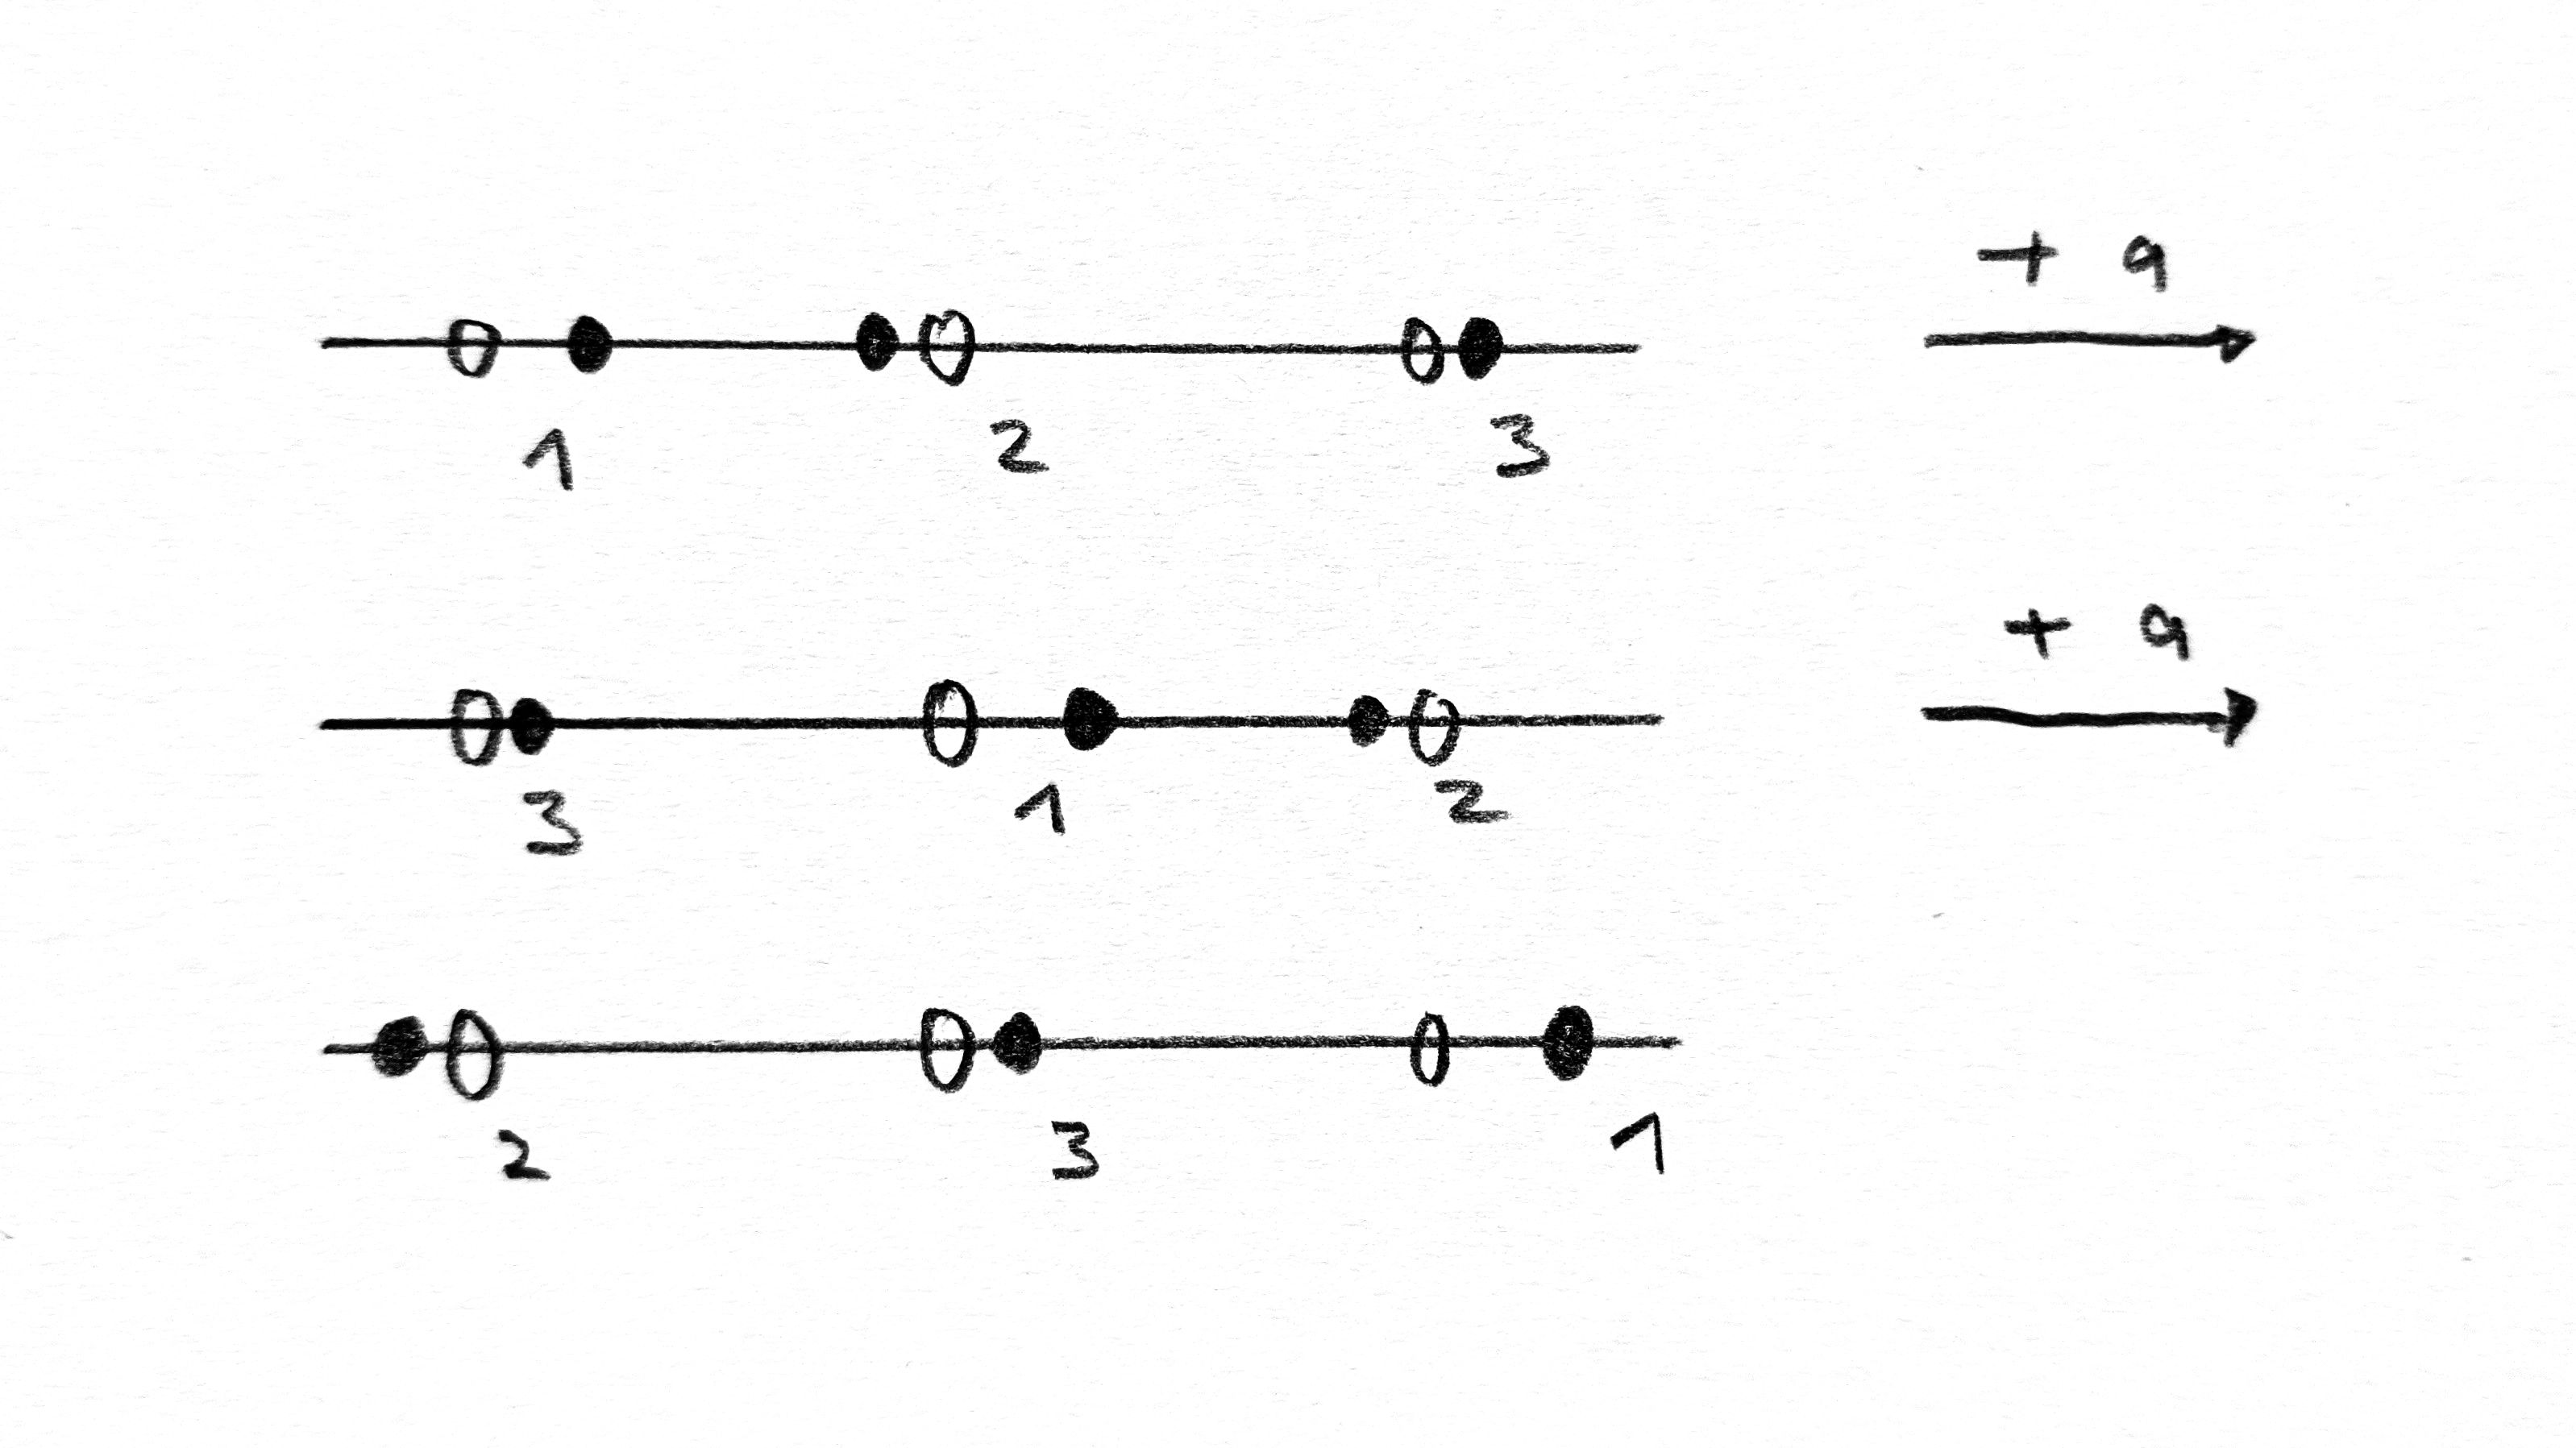
\includegraphics[width=.68\textwidth]{./sketches/permutation1.jpg}
	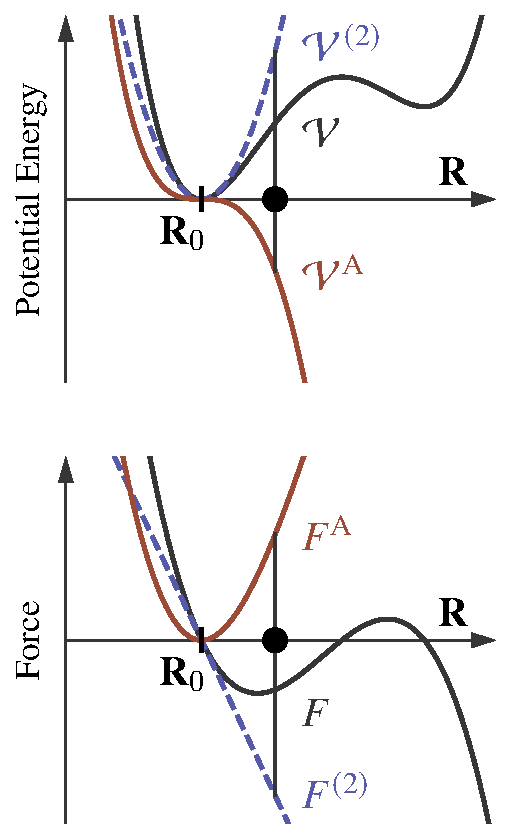
\includegraphics[width=\textwidth]{./data/plots/anharmonicity/1_pes_sketch/sketch_vertical.pdf}
	\caption{Upper: Sketch of a one-dimensional potential-energy surface $\mathcal V$ (solid black), its harmonic approximation $\mathcal{V}^{(2)} (\b R)$ (dashed blue), and the anharmonic contribution $\mathcal{V}^{\rm A} (\b R)$ (solid red). Right: The force ${F} ({\bf R})$ given by the derivative of the potential energy $\mathcal V$ (black), the force $F^{(2)}$ stemming from the harmonic potential $\mathcal{V}^{(2)} (\b R)$ (blue), and the anharmonic contribution $F^\mathrm{A} = F - F^{(2)}$ (red), cf.~Eq.\,\eqref{eq:anh.F}.}
	\label{fig:pes_sketch_vertical}
\end{marginfigure}


\section{Anharmonicity measure}

We base the discussion of anharmonicity in the following on the forces, for two reasons: First, because the dynamical evolution of the system is determined by the potential through the equations of motion, and therefore by the gradients,~i.\,e.,~the forces. Second, because the forces give more microscopic insight, as they can be resolved per atom, and better statistic, since per configuration $\bf R$, there are $3N$ force components ${\bf F} = ({\bf F}_1, \ldots, {\bf F}_N)$.

In terms of the force contributions defined in Eq.\,\eqref{eq:anh.F}, we define a \emph{measure of anharmonicity} in the following way:
\begin{align}
	\sigmaA (T)
		% = \frac{\sigma [F^{\rm A}]_T}{\sigma [F]_T}
		= \sqrt{\frac{\sum_{I, \alpha} \braket{(F^{\rm A}_{I, \alpha})^2}_T}{\sum_{I, \alpha} \braket{(F_{I, \alpha})^2}_T}}~,
	\label{eq:sigmaA}
\end{align}
where $F_{I, \alpha}^{(A)}$ is the $\alpha$ component of the (anharmonic) force on atom $I$, and $\braket{\cdot}_T$ denotes a thermodynamic average at temperature $T$. The interpretation of the measure $\sigmaA$ is that it quantifies the anharmonic strength in terms of the standard deviation of the distribution of anharmonic force components at a given temperature, $\sigma [F^{\rm A}]_T$, normalized by the standard deviation of the actual force distribution, $\sigma [F]_T$, where the standard deviation of force distributions is defined as
\begin{align}
	\sigma [F]_T 
		= \sqrt{\frac{1}{3N} \sum_{I, \alpha} \braket{F_{I, \alpha}^2}_T}~.
\end{align}
The effect of normalizing the distribution of forces is shown in Fig.\,\ref{fig:anh.normalization} for the two exemplary materials already discussed in the context of phonon dispersions in Sec.\,\ref{sec:ha.dispersions}, fcc-silicon, and the orthorombic perovskite KCaF$_3$.
\begin{marginfigure}
	\centering
	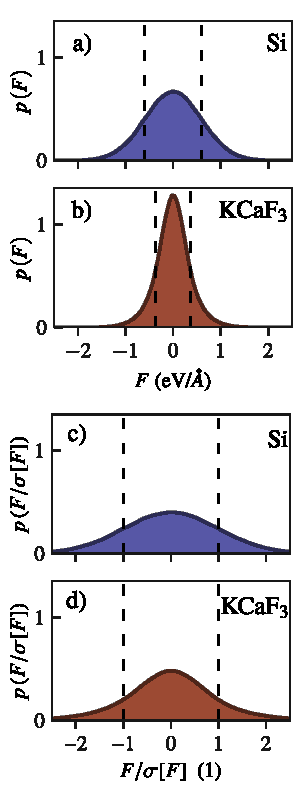
\includegraphics[width=0.8\textwidth]{./data/plots/anharmonicity/4_force_distribution/histogram_forces_vertical.pdf}
	\caption{
		Force component distribution before and after normalization with the width of the distribution $\sigma [F]$. $p(F)$ denotes the probability to find a force component $F_{I, \alpha}$ of strength $F$ in the material. Panel a) and b) show the distribution before normalization, c) and d) after normalization. Dashed vertical lines denotes the standard deviation of the displayed distribution.
	}
	\label{fig:anh.normalization}
\end{marginfigure}
For these two materials, we show the normalized distributions of forces and anharmonic force contributions in Fig.\,\ref{fig:anh.sigmaA}.
\begin{figure}
	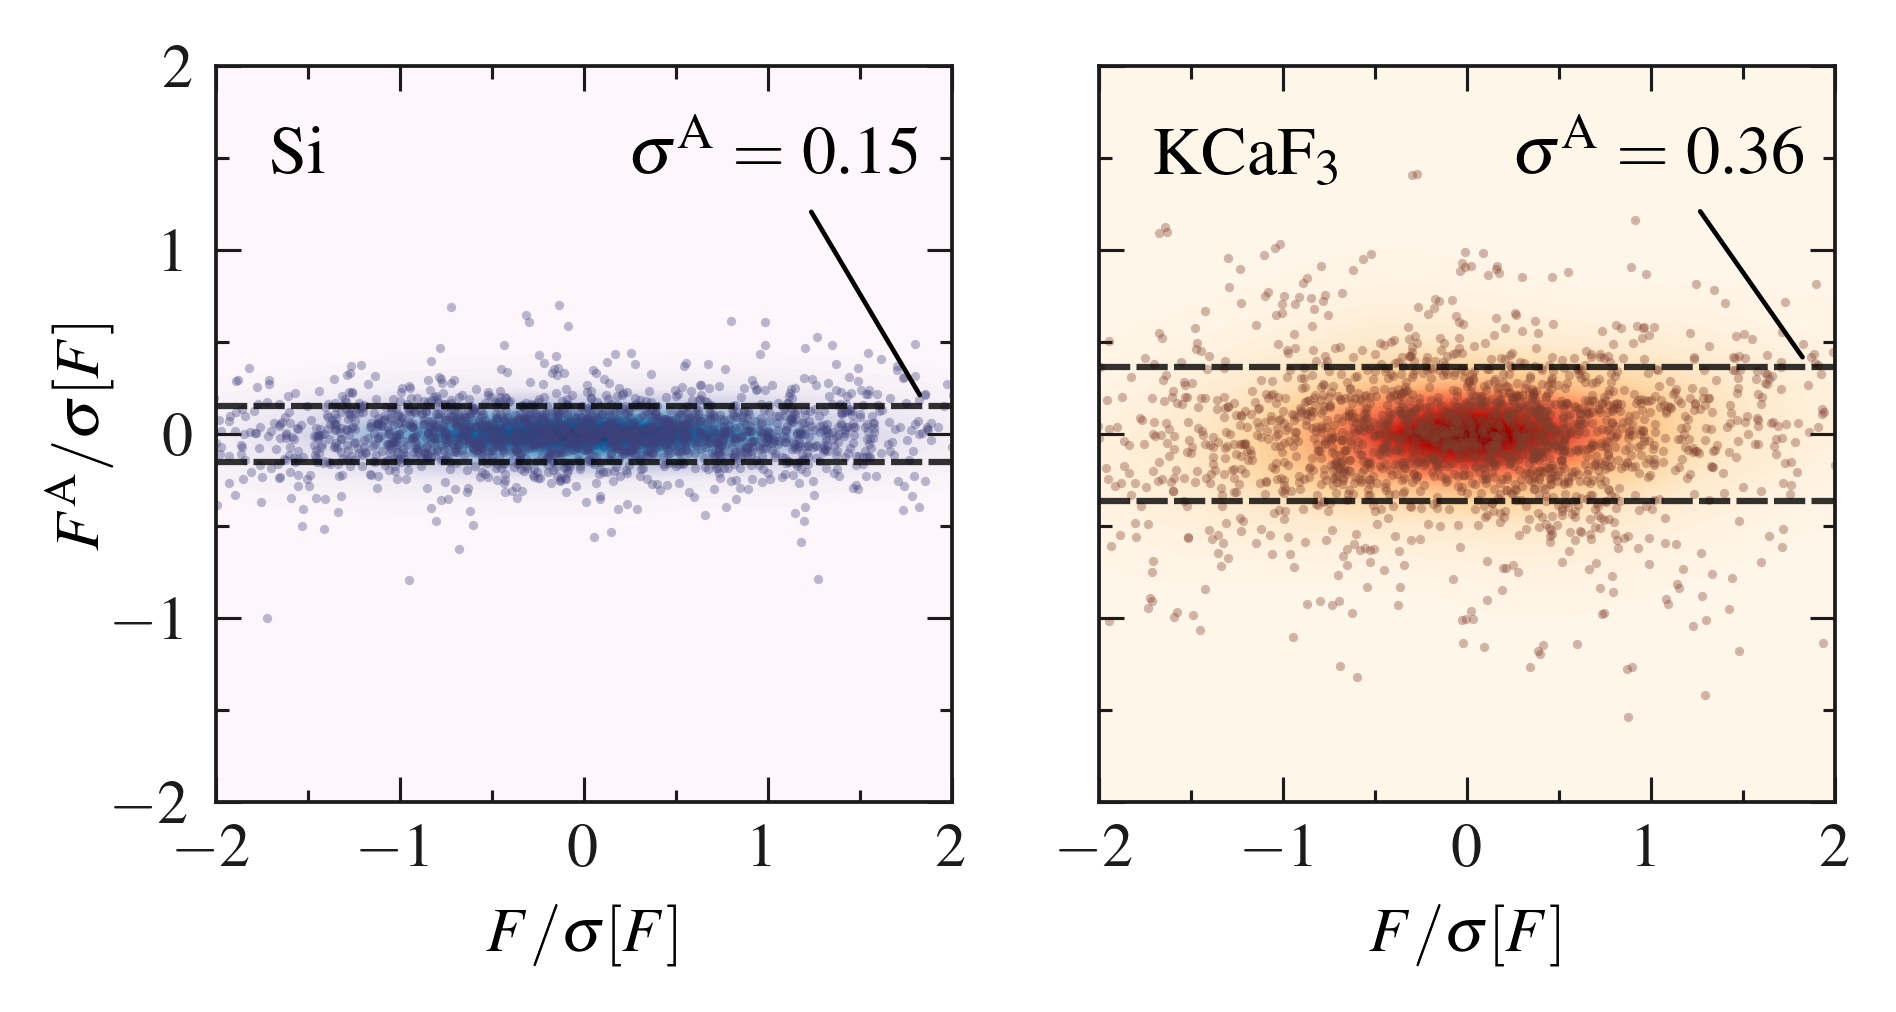
\includegraphics[width=\textwidth]{./data/plots/anharmonicity/5_density_plots/histogram_annotated.png}
	\caption{
		Normalized anharmonic force components versus normalized force components. Dashed horizontal lines: Width of the distribution estimated from standard deviation. Individual dots are force components sampled during an \emph{ab initio} MD simulations.
	}
	\label{fig:anh.sigmaA}
\end{figure}
In this visualization, the measure of anharmonicity $\sigmaA$ is given by the standard deviation of the distribution in y-direction, as indicated by the dashed vertical lines in the plot. The distribution of anharmonic force components is more than twice as broad for the perovskite KCaF$_3$ compared to silicon, with $\sigmaA$ of 0.36 compared to 0.15, respectively. This can be interpreted in the sense that 36\,\% of the forces stem from anharmonic contributions in KCaF$_3$, and 15\,\% in silicon. Furthermore, strongly anharmonic force contributions with a strength of $0.5\,\sigma [F]$ or more are nearly absent in silicon with a probability of $<0.01\,\%$, whereas anharmonic forces of this strength in KCaF$_3$ occur with a much higher probability of $\sim 16.5\,\%$.


\newthought{The anharmonicity measure defined in Eq.\,\eqref{eq:sigmaA}} can also be evaluated for subsets of the dynamical degrees of freedom,~e.\,g.,~per chemical species, as shown in Fig.\,\ref{fig.anh.sigmaA.atoms}.
\begin{figure}
	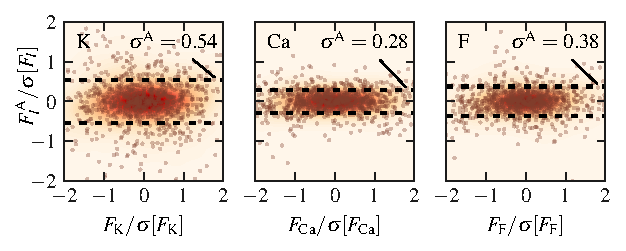
\includegraphics[width=\textwidth]{./data/plots/anharmonicity/5_density_plots/histogram_atoms.pdf}
	\caption{
		Normalized anharmonic force components versus normalized force components. Dashed horizontal lines: Width of the distribution estimated from standard deviation.
	}
	\label{fig.anh.sigmaA.atoms}
\end{figure}
In the example of KCaF$_3$, this analysis shows that the calcium (Ca) atoms occupying the vertices of the unit cell are comparatively stable, whereas potassium (K) is located in a shallow potential, which can be explained by the phase-transition mechanism observed in KCaF$_3$: Above 560\,K, the material becomes cubic, and the octahedral displacement of fluorine~(F) is removed~\cite{Bulou1980,Hidaka1984}. As shown in Fig.\,\ref{fig:anh.KCaF3}, this tilt also affect the potassium atoms, which are displaced from their high-temperature reference position.
\begin{marginfigure}
	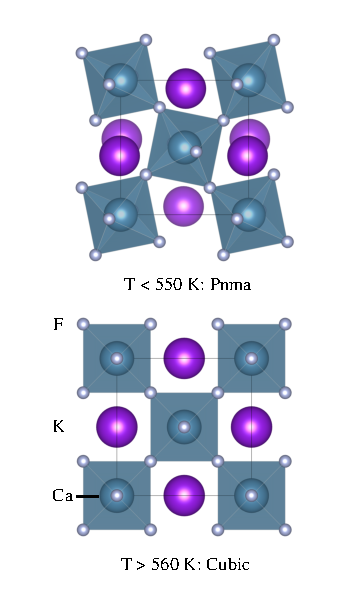
\includegraphics[width=\textwidth]{./data/plots/anharmonicity/2_materials/both.pdf}
	\caption{
		\label{fig:KCaF3}
		KCaF$_3$ in the low-temperature Pnma~(top) and high-temperature cubic phase~(bottom). Both structures are viewed along the long $b$-axis.
	}
	\label{fig:anh.KCaF3}
\end{marginfigure}

\newthought{Furthermore, it is instructive to evalute the anharmonicity for single configurations}, be it snapshots in time during molecular dynamics simulations, or when using other sampling approaches,~e.\,g,~harmonic Monte Carlo samples as defined in Eq.\,\eqref{eq:ha.samples}. While we will discuss ``time-resolved anharmonicity'' in detail at a later point, we show the evaluation of $\sigmaA$ for samples generated by Eq.\,\eqref{eq:ha.samples} in Fig.\,\ref{fig:anh.sampling}.
\begin{figure}
	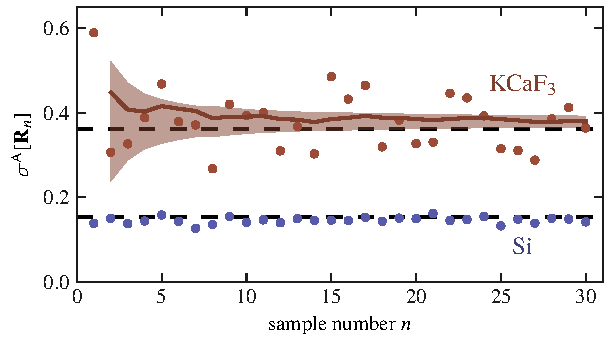
\includegraphics[width=4.1in]{./data/plots/anharmonicity/7_sampling/convergence_sigma_MC.pdf}
	\caption{
			Anharmonicity measure $\sigmaA$ evaluated for individual atomic configurations obtained from Eq.\,\eqref{eq:ha.samples}. Dots: $\sigmaA [{\bf R}_n]$ for individual samples; Red line: Cumulative average.	Black dashed line: $\sigmaA$ from \emph{ai}MD.	Shadowed region: Convergence estimated by standard error.
	}
	\label{fig:anh.sampling}
\end{figure}
The analysis shows that a decent estimate of the anharmonicity measure $\sigmaA$ can be obtained from the harmonic sampling analysis with few samples, especially for silicon, where every individual harmonic sample yielded a $\sigmaA$ within 99\,\% of the reference value obtained by MD simulation for several hundred simulation time steps indicated by the dashed vertical line. For the more anharmonic KCaF$_3$, the harmonic sampling with 30~samples yields an estimated value of $\sigmaA_{\rm est.} = 0.38$, which differs from the MD value ($\sigmaA = 0.36$) by about 5\,\%. A distinction between largely harmonic materials like silicon, and anharmonic materials like KCaF$_3$ is therefore possible with very few samples

\newthought{Motivated by this fact, investigated the possiblity to estimate $\sigmaA$ based on a single samples}, as suggested by Zacharias and coworkers in Ref.\,\cite{Zacharias2016}, where a single, deterministic sample probing the most probable part of the harmonic distribution is used by using a fixed $\zeta_s = (-1)^s)$ instead of a random distribution in Eq.\,\eqref{eq:ha.samples}. We denote anharmonicity measures obtained by such a ``one-shot'' approach by $\sigmaAOS$ in the following. As shown in Fig.\,\ref{fig:anh.one-shot}, the one-shot samples provide very good estimates for silicon in the the entire temperature range from 200\,K to 800\,K, which can be expected due to the largely harmonic nature of silicon.
\begin{figure}
	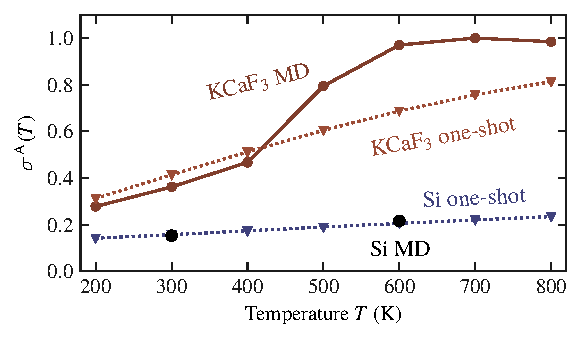
\includegraphics[width=4.1in]{./data/plots/anharmonicity/7_sampling/sigma_temp_one_shot.pdf}
	\caption{
		$\sigmaA$ as a function of temperature obtained from MD~simulations (black circles) and one-shot sampling (triangles connected by dashed curves)
	}
	\label{fig:anh.one-shot}
\end{figure}
For KCaF$_3$, the agreement is good in the temperature range from 200\, to 400\,K, at least within the limits of the harmonic sampling approach as discussed in the previous paragraph, taking into account that only a single sample was used. Above 500\,K, however, the difference to the reference value from MD simulations increases, which is due to the phase transition occuring in KCaF$_3$ discussed earlier, which also occurs in the simulation cell. A prediction of anharmonicity across phase transitions can therefore not be expected, which can be expected by noting that the entire reference frame for the harmonic model changes when a phase transition occurs. The phase transition mechanism of KCaF$_3$ and implications for the anharmonicity measure are further discussed in Ref.\,\cite{Knoop2020}.

\newthought{Ultimately, the applicability of the one-shot sampling approach} needs to be assessed for a diverse set of materials, especially if one aims to use this scheme to screen for anharmonicity in material space. As shown in Fig.\,\ref{fig:anh.screening} for a set of 63~materials, the one-shot sampling is reliable within $\pm 10\,\%$ for all materials in the set up to a value of about $\sigmaA \simeq 0.3$.
\begin{figure}
	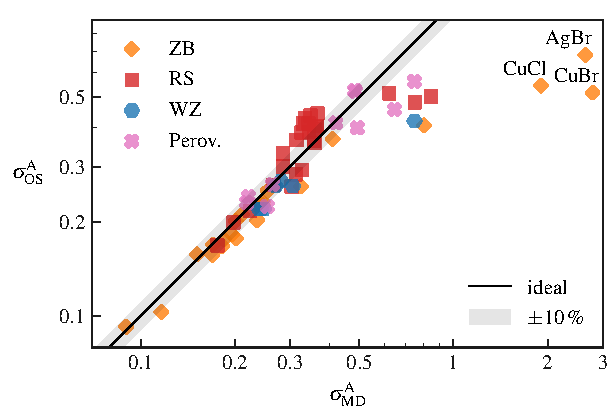
\includegraphics[width=4.1in]{./data/plots/anharmonicity/8_screening/sigma_os_md.pdf}
	\caption{
		Comparison of the anharmonicity measure obtained from MD simulations and one-shot sampling (OS) for 63 materials at 300\,K. The set comprises 25 rock salt (RS), 21 zincblende (ZS), 7 wurtzite (WZ), and 10 orthorombic perovskite (Perov.) materials. The diagonal line denotes perfect agreement between MD and OS, and the green area denotes a 10\,\%~error margin to guide the eye.
		Data was taken from Ref.\,\cite{Knoop2020}.
	}
	\label{fig:anh.screening}
\end{figure}
For larger values of $\sigmaA$, the deviation can become larger, especially for the rock salt materials with $\sigmaA \simeq 0.35$ which the one-shot sampling overestimates by about 20\,\%. Nevertheless, the agreement is qualitatively correct up to values of about $\sigmaA \simeq 0.5$, after which materials begin to show effects not captures by the harmonic sampling,~e.\,g.,~phase transition as discussed earlier for KCaF$_3$. In particular, the three highlighted noble metal halides AgBr, CuCl, and CuBr deviate strongly. These materials tend towards non-perturbative effects during the MD simulation such as spontaneous defect formation~\cite{Knoop2020}, which is a dynamical effect impossible to be described by any reference harmonic model. We will discuss the nature of these effects in more detail later. To conclude, we point out that also in the case of non-trivial dynamical effects such as defect formation, the estimated anharmonicity scored $\sigmaAOS$ are larger than $\gtrapprox 0.5$, and therefore indicate strong anharmonicity. Classifying strong anharmonicity in terms of one-shot sampling, $\sigmaAOS$, is therefore possible for all materials in the set.


\subsection{Anharmonicity and thermal conductivity}

Based on the qualitative discussion of thermal transport in Sec.\,\ref{sec:hf.kappa.ha}, one can expect that stronger anharmonicity leads to shorter phonon lifetimes and therefore lower thermal conductivity. We tested this hypothesis for a list of 47 materials where experimental reference was available~\cite{Morelli2006,Chen2019}. The results are shown in Fig.\,\ref{fig:anh.kappa}.
\begin{figure}
	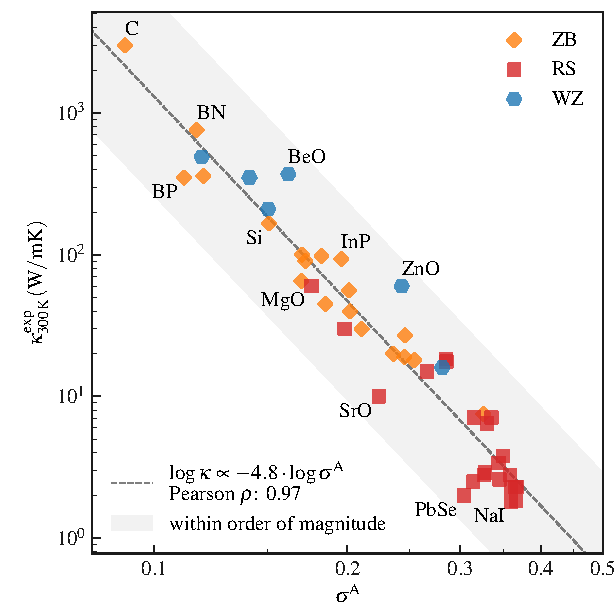
\includegraphics[width=4.1in]{./data/plots/anharmonicity/9_kappa/sigma_vs_kappa.pdf}
	\caption{
		Experimental thermal conductivity at room temperature, $\kappa^{\rm exp}_{300\,{\rm K}}$, versus one-shot measure of anharmonicity, $\sigmaAOS$. The dashed diagonal line indicates a power law fit for the data. The grey area denotes values of $\kappa$ which agree with the fit within an order of magnitude. The dataset contains 47 materials, 22 rock salt (RS), 19 zincblende (ZB), and 6 wurtzite (WZ) structures. Experimental data from Ref.~\cite{Morelli2006,Chen2019}.
	}
	\label{fig:anh.kappa}
\end{figure}
The analysis reveals an inverse power law relationship between thermal conductivity and anharmonicity for the materials in the dataset. Given that just a single descriptor was used,~i.\,e.,~the estimated anharmonicity score, and not further vibrational properties as commonly employed in semi-empirical models for thermal condcutivity\CITE{Curtarolo,Toberer,Ramprasad}, this observation is too some extent surprising, although encouraging that $\sigmaA$ captures some essential physics relevant to heat transport.

\newthought{The most important messages from Fig.\,\ref{fig:anh.kappa} can be summarized as follows}:
\begin{enumerate}
	\item Largely harmonic materials with $\sigmaA \simeq 0.1$, like diamond (C), boron nitride (BN), or boron phosphide (BP) can be expected to be good thermal conductors with $\kappa \gtrsim 100\,{\rm W/mK}$.
	\item Strongly anharmonic materials with $\sigmaA \gtrsim 0.3$ can be expected to be poor thermal conductors with $\kappa \lesssim 10\,{\rm W/mK}$, if one adopts the definition suggested by Morelli and Slack to define ``high thermal conductivity'' as $\kappa \gtrsim 50 \, {\rm W/mK}$~\cite{Morelli2006}.
	\item $\sigmaA$ has a strong correlation with thermal conductivity across the entire dataset, but nevertheless only a rough estimate can be made, especially in the middle region with $\sigmaA \simeq 0.2$. This can be best seen by comparing strontium oxide (SrO) with $\kappa = 10\,{\rm W/mK}$ and $\sigmaA = 0.22$, and zinc oxide (ZnO) with $\kappa = 60\,{\rm W/mK}$ and $\sigmaA = 0.24$, or beryllium oxide (BeO) with $\kappa = 370\,{\rm W/mK}$ and $\sigmaA = 0.16$ to magnesium oxide (MgO) with $\kappa = 60\,{\rm W/mK}$ and $\sigmaA = 0.18$. These pairs of materials differ only slightly in their estimated anharmonicity, but still quite strongly in the thermal conductivity. 
\end{enumerate}

\newthought{These findings suggest the following approach} towards screening material space in search for thermal insulators: Estimate the anharmonicity for materials of interest and discard the largely harmonic ones, as they will be good thermal conductors most of the time. Of course, the reverse approach can be pursued when searching for materials with potentially high thermal conductivity.

\subsection{Candidate Materials}
\begin{marginfigure}
	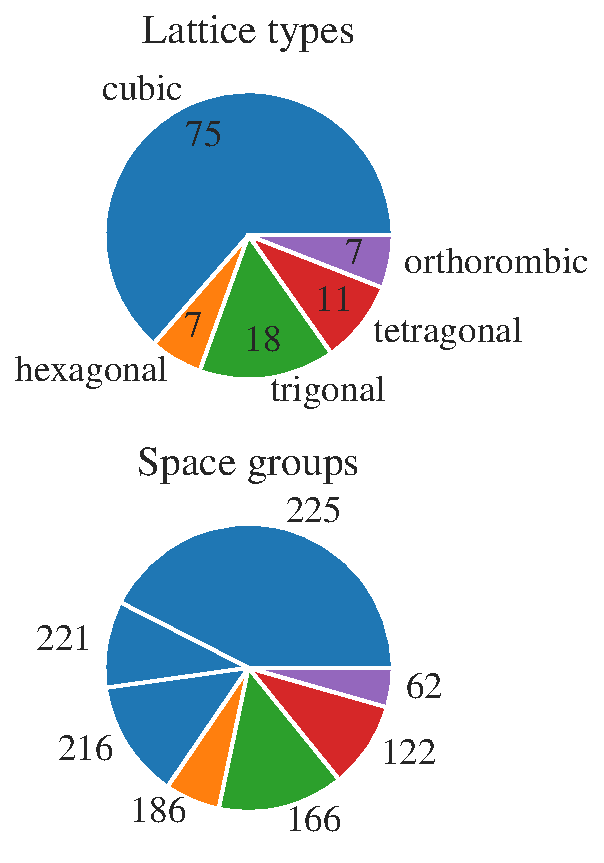
\includegraphics[width=\textwidth]{./data/plots/dataset/pies.pdf}
	\caption{
		Lattice types and space groups represented in the dataset. Space groups not shown in the pie chart: 56, 61, 160, 164, 206, with one representative each.
	}
	\label{fig:anh.pie}
\end{marginfigure}
In the context of the work published in Ref.\,\cite{Knoop2020}, we have identified a set of 118 binary and ternary materials for further investigation with the \emph{ab intio} Green Kubo (aiGK) approach. The materials comprises five lattice types and 12 space groups as summarized in Fig.\,\ref{fig:anh.pie}.  Since we are mainly interested in thermal insulators as candidate thermoelectric and thermal barrier coating materials, we have discarded largely harmonic materials with $\sigmaA < 0.17$ from the set, and focus on anharmonic strengths $\sigmaA > 0.2$ with a mean of $\sigmaA=0.31$ and a median of $\sigmaA = 0.29$. A histogram displaying the distribution of $\sigmaA$ values is shown in Fig.\,\ref{fig:anh.histogram}.
\begin{figure}
	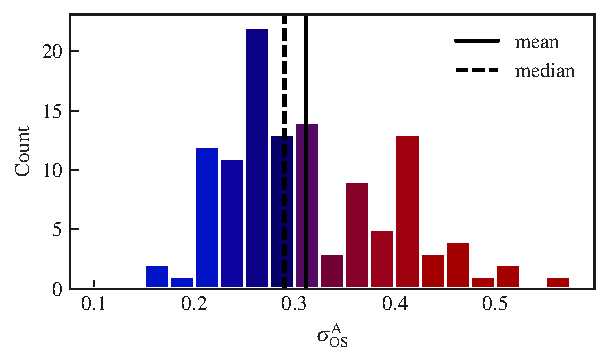
\includegraphics[width=4.1in]{./data/plots/dataset/histogram.pdf}
	\caption{
		Histogram of $\sigmaAOS$ values samples for the 118 chosen materials
	}
	\label{fig:anh.histogram}
\end{figure}
All values are given with respect to room temperature, as this is the regime where the most experimental reference is available to benchmark the aiGK method and to showcase the approach. In total, there are experimental reference values for 45 materials available, were we have discarded sources of questionable quality.

The materials come from these sources:
From Ramprasad: 41
From Toberer: 3
From Springer: 4
From Roekeghem: 9
From ICSD: 55
From Seko: 2
From AAPL: 4


% \part{Benchmarks?}

% \part{Results}
\chapter{Screening Materials for Anharmonicity}
\section{Screening Material Space}

\subsection{Preparation: Efficient Sampling of Anharmonicity}

\begin{figure}
	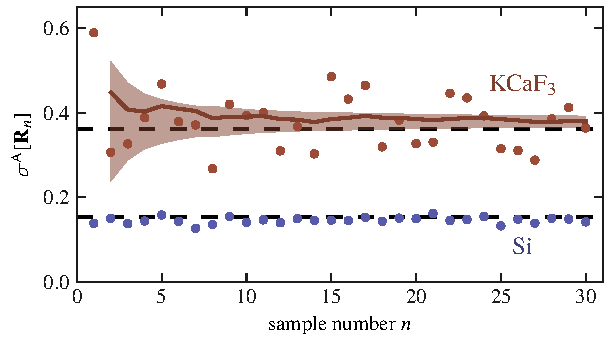
\includegraphics[width=4.1in]{./data/plots/anharmonicity/7_sampling/convergence_sigma_MC.pdf}
	\caption{
		Some text to describe the figure.
	}
\end{figure}

\begin{figure}
	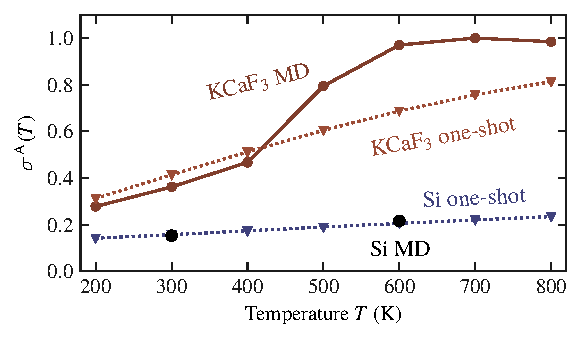
\includegraphics[width=4.1in]{./data/plots/anharmonicity/7_sampling/sigma_temp_one_shot.pdf}
	\caption{
		Some text to describe the figure.
	}
\end{figure}

\begin{figure}
	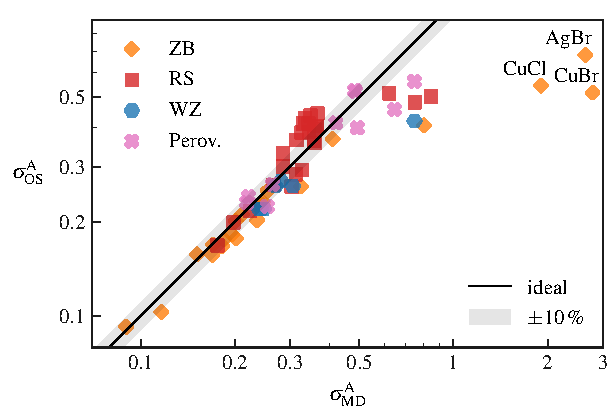
\includegraphics[width=4.1in]{./data/plots/anharmonicity/8_screening/sigma_os_md.pdf}
	\caption{
		Some text to describe the figure.
	}
\end{figure}

\subsection{Literature Review}
Lorem ipsum dolor sit amet, consetetur sadipscing elitr, sed diam nonumy eirmod tempor invidunt ut labore et dolore magna aliquyam erat, sed diam voluptua. At vero eos et accusam et justo duo dolores et ea rebum. Stet clita kasd gubergren, no sea takimata sanctus est Lorem ipsum dolor sit amet. Lorem ipsum dolor sit amet, consetetur sadipscing elitr, sed diam nonumy eirmod tempor invidunt ut labore et dolore magna aliquyam erat, sed diam voluptua. At vero eos et accusam et justo duo dolores et ea rebum. Stet clita kasd gubergren, no sea takimata sanctus est Lorem ipsum dolor sit amet.

\begin{figure}
	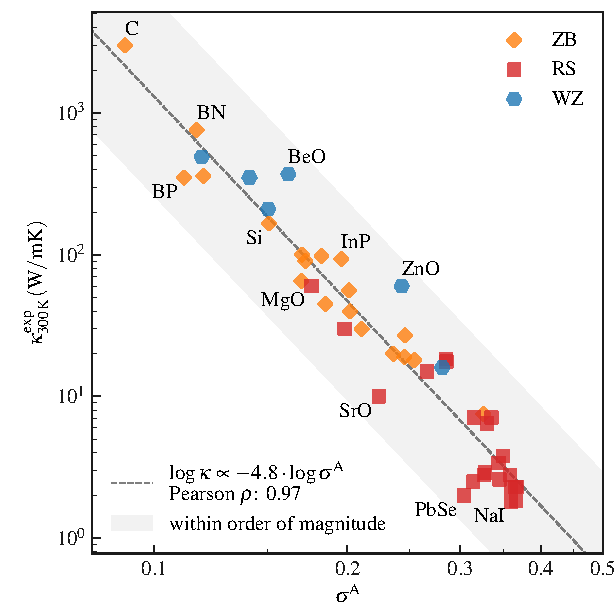
\includegraphics[width=4.1in]{./data/plots/anharmonicity/9_kappa/sigma_vs_kappa.pdf}
	\caption{
		Some text to describe the figure.
	}
\end{figure}

Lorem ipsum dolor sit amet, consetetur sadipscing elitr, sed diam nonumy eirmod tempor invidunt ut labore et dolore magna aliquyam erat, sed diam voluptua. At vero eos et accusam et justo duo dolores et ea rebum. Stet clita kasd gubergren, no sea takimata sanctus est Lorem ipsum dolor sit amet. Lorem ipsum dolor sit amet, consetetur sadipscing elitr, sed diam nonumy eirmod tempor invidunt ut labore et dolore magna aliquyam erat, sed diam voluptua. At vero eos et accusam et justo duo dolores et ea rebum. Stet clita kasd gubergren, no sea takimata sanctus est Lorem ipsum dolor sit amet.

\subsection{Candidate Materials}

\chapter{Thermal Conductivities for Strongly Anharmonic Compounds}
\label{chp:results}

After introducing the implementation of the \emph{ab initio} Green Kubo (aiGK) method in the previous chapter, we are now in position to present results for the set of potential thermal insulators identified in chapter~\ref{chp:anharmonicity}.

We first discuss the question of simulation time convergence for an initial set of materials in order to predict systems which can be computed with a simulation time of 30-60\,ps. This time was chosen as a compromise between the finite amount of available computational ressources and the desire to compute as many materials from the list of candidates as possible.
% 57 materials
%
In a second step, we compare the computed thermal conductivities at room temperature to experimental references for the subset of materials for which experiments are available to further verify the aiGK method beyond the two materials presented in the previous chapter.
% 22 materials 
%
In the last step, we present the computed thermal conductivities for the remaining materials,~i.\,e.,~those for which no experimental thermal conductivity was reported before, and discuss how they fit into the schema of predicting thermal insulators from anharmonicity estimates as discussed in Sec.\,\ref{sec:kappa_vs_sigmaA}. We eventually highlight the particularly interesting class of chalcopyrite compounds and try to answer some open questions from experimental and semi-empirical theoretical literature.

% \idea{compare to theoretical approaches, i.e., the Roekeghem perovskites}



\section{Convergence estimation}
We discuss simulation time convergence in the light of the \emph{effective simulation time} introduced in Sec.\,\ref{sec:implementation.convergece}. The key idea is to identify lower boundaries for the \emph{necessary} effective simulation time in a material in order to asses whether a time-converged thermal conductivity is possible to obtain within a simulation time of 30-60\,ps. For choosing these boundaries, we leverage the observed convergence behavior of seven materials,~i.\,e.,~MgO, NaF, KMgF$_3$, NaCl, NaBr, CuI, and NaI, each of them computed with 60\,ps simulation time. We thereby define four thresholds of minimal effective simulation time based on a material's anharmonicity $\sigmaA$, reflecting that phonons in harmonic materials like MgO have longer lifetimes than those in anharmonic materials. The criteria are displayed in Fig.\,\ref{fig:results.convergence}. In particular, we define the thresholds $\teff > 240$ for harmonic materials with $\sigmaA \leq 0.2$, $\teff > 120$ for materials with $0.2 < \sigmaA \leq 0.3$, $\teff > 60$ for materials with $0.3 < \sigmaA \leq 0.4$, and $\teff > 45$ for materials with $\sigmaA > 0.4$.

%The rational for this approach is that for individual materials, one would always compute several times longer trajectories to ensure that all relevant contributions are captured. In turn, several times less materials could be computed with a given amount of computational resources. Here, we leverage observations across different materials to circumvent this necessity for individual materials, thereby allowing to compute good estimates for thermal conductivity for dozens of them.
%
\begin{figure}
	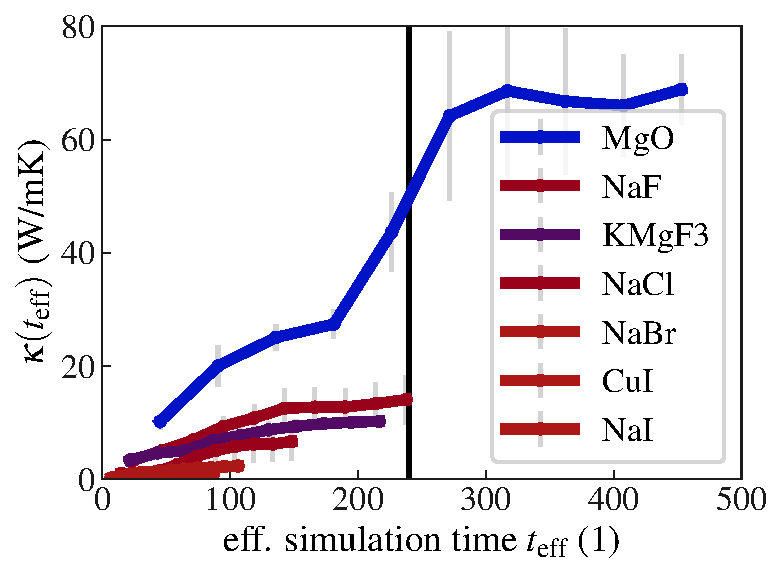
\includegraphics[width=.49\textwidth]{./data/plots/kappa_convergence/3.pdf}
	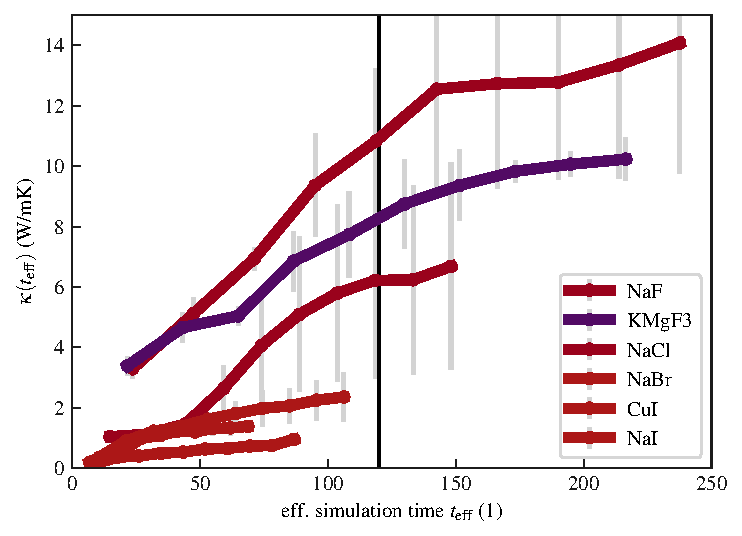
\includegraphics[width=.49\textwidth]{./data/plots/kappa_convergence/4.pdf}
	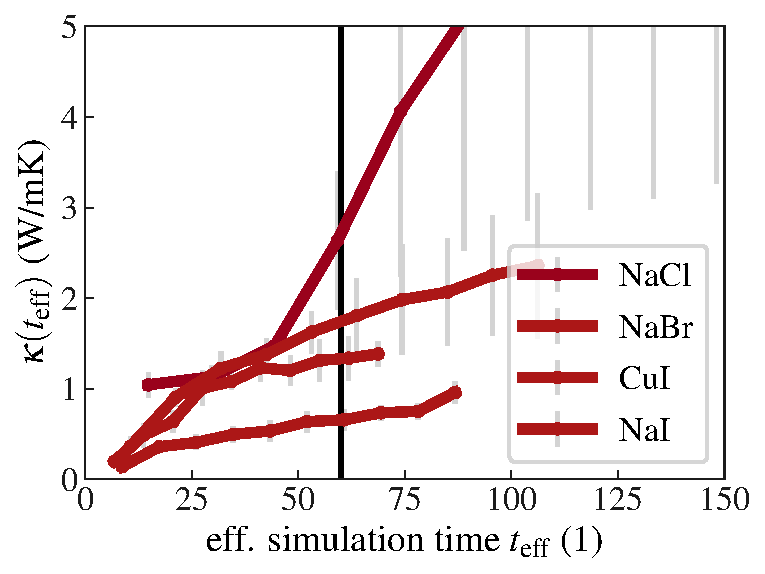
\includegraphics[width=.49\textwidth]{./data/plots/kappa_convergence/5.pdf}
	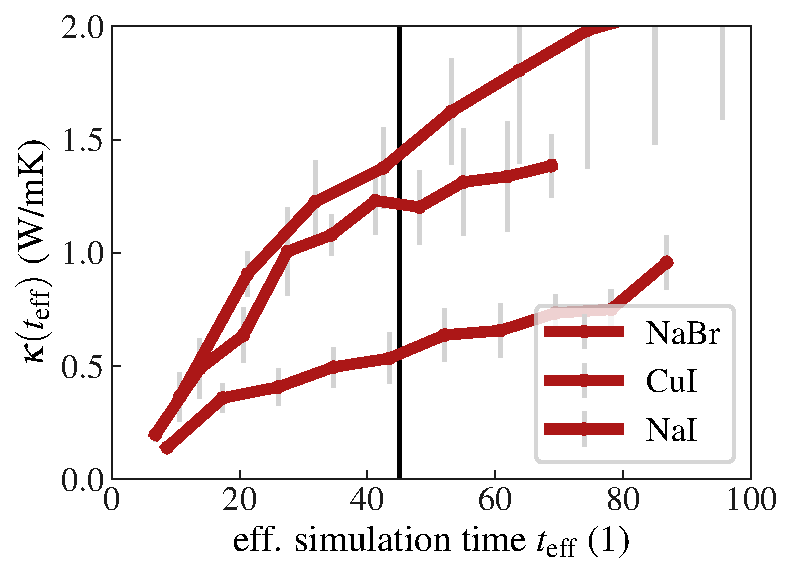
\includegraphics[width=.49\textwidth]{./data/plots/kappa_convergence/6.pdf}
	\caption{Illustration of minimal necessary effective simulation times. Upper left: $\teff = 240$ for harmonic materials with $\sigmaA \leq 0.2$. Upper right: $\teff = 120$ for materials with $0.2 < \sigmaA \leq 0.3$. Lower left: $\teff = 60$ for materials with $0.3 < \sigmaA \leq 0.4$. Lower right: $\teff = 45$ for materials with $\sigmaA > 0.4$.}
	\label{fig:results.convergence}
\end{figure}
%
We point out that at this stage, the given thresholds are meant as a \emph{necessary} condition for convergence, which ensures that a significant contribution to the cumulative thermal conductivity is included in the simulation. A statement about the \emph{sufficient} simulation time, however, can only made on the level of individual trajectories by means of longer simulation times. This verification should therefore be reserved for materials that show interesting properties after the \emph{necessary} simulation time.

Based on this estimation, we identify 57~materials out of the list of 112~candidates to compute thermal conductivity on, and discuss those in the following: First we compare thermal conductivities for 24 of these 57 materials to the experimental literature in order to benchmark the aiGK method, afterwards we present and discuss our findings for the remaining 33 materials without experimental reference.
\TODO{list of materials in appendix}



\section{Comparison to Experiment}
\label{sec:results.experiments}
In order to asses the validity of the aiGK method for the computation of thermal conductivity in anharmonic compounds, we compare results for 21 materials to the experimental literature. A detailed list including all considered experimental references is given in Tab.\,\ref{tab:kappa.exp} in appendix~\ref{sec:app.experiments}. The difficulties when comparing to experimental references have been discussed in detail for periclase MgO in Sec.\,\ref{sec:mgo.experiments}. In principle, these carry over to all other compounds, however, for most materials, the body of literature is much smaller compared to MgO. The list of experiments also includes measurements on polycrystalline samples. While thermal conductivity should be reduced in polycrystalline samples compared to single crystals because of boundary scattering, experimental studies have shown that the effect is minor in sufficiently dense polycrystalline samples, especially in low thermal conductivity materials which are less sensitive to boundary scattering due to their intrinsically low phonon mean free paths~\cite{Charvat.1957}. In the course of our literature review we have generally found differences of 0-20\,\% between measurements on single- and polycrystalline samples, which supports this finding. Nevertheless, additional care must be taken when evaluating literature on polycrystalline samples: Experiments aiming at measuring other properties besides thermal conductivity, in particular the thermoelectric figure of merit $zT$, typically do not attempt to reproduce the bulk thermal conductivity, and use less dense samples, which is beneficial for reducing thermal conductivity and thereby increasing the figure of merit. The resulting thermal conductivity will then be determined mostly by the details of the sample processing, 
%\mscomment{this is true for all experimental data}
%\FK{I disagree, actual bulk properties are somewhat robust against minor manufacturing differences. Clarify: I mean here that sampling process \emph{significanlty} determines the properties beyond single-digit deviations.}
and a comparison to bulk thermal conductivity is not meaningful. However, some experiments specifically aim at reproducing polycrystalline samples of near-bulk density in order to assess the bulk thermal conductivity of a material. Only experiments on polycrystalline samples of this type are considered in this work.

A comparison of thermal conductivities computed via the aiGK method as introduced in the previous chapter and the experimental literature is shown in Fig.\,\ref{fig:kappa_exp}.
%
\begin{figure}
	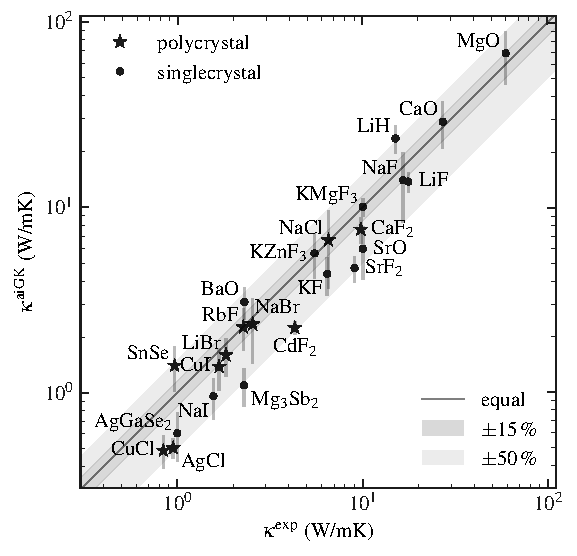
\includegraphics[width=\textwidth]{./data/plots/kappa_vs_exp_trusted/kappa_vs_exp_corrected_annotated.pdf}
	\caption{Comparison to experiment. Bullets($\bullet$): Single crystal. Stars ($\star$): Contains data from polycrystalline experiment. Error bar in y-direction: Statistical uncertainty for $\kappa^{\rm aiGK}$ from standard error over individual trajectories. Diagonal line: Agreement with experiment or mean of experiments if multiple available. Dark grey region: Agreement between mean experiment and mean computation with $\pm 15\,\%$ deviation. Light grey region: Agreement between mean experiment and mean computation with $\pm 50\,\%$ deviation.}
	\label{fig:kappa_exp}
\end{figure}
%
Overall, we find very good agreement in the 24 considered materials, with 10 out of 24 being within experimental accuracy of $\pm 15\,\%$, and all other within an extended %experimental 
accuracy which we choose as $\pm 50\,\%$ within the average experimental reference, reflecting the high degree of variation in experimental values for materials where a significant amount of references is available, see our discussion for MgO in Sec.\,\ref{sec:mgo.experiments} and the discussion in Ref.\,\cite{Wei.2016}. 

\begin{marginfigure}
	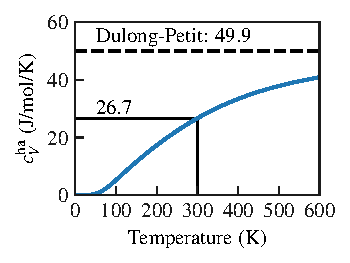
\includegraphics[width=\textwidth]{./data/plots/heat_capacity/225.LiH/thermal_properties.pdf}
	\caption{Harmonic heat capacity per formula unit $c_V^{\rm ha}$ for LiH compared to the classical Dulong-Petit value.}
	\label{fig:LiH.cv}
\end{marginfigure}
%
The strongest deviation from experiment is seen for LiH, which is computed as $\kappa^{\rm aiGK} = 23.6 \pm 4.0$\,W/mK, where the available experimental value is $\kappa^{\rm exp} = 14.7$\,W/mK~\cite{Slack.1973}. However, both lithium and especially hydrogen are light elements, so that LiH is not fully classical at room temperature, as can be estimated by comparing the harmonic heat capacity of LiH at 300\,K to the classical Dulong-Petit value in Fig.\,\ref{fig:LiH.cv}~\cite{Dove}. The harmonic heat capacity for LiH is only at about 50\,\% of the classically expected value of $6 R = 49.9$\,J/mol/K for solids with two atoms in the unitcell. This value can only be taken as an upper boundary to the deviation in thermal tranpsort properties expected from the lack of nuclear quantum effects, since low-frequency phonon modes already behave more classical at the given temperature~\cite{Volz.2020,Volz.2020b}. A significant overestimation by the classical Green Kubo method can nevertheless be expected in this material.\footnote{We evaluated several schemes to quantitatively correct for nuclear quantum effects~\cite{Wang.1990,Maiti.1997}, however, the literature seems to agree that this is an open problem for thermal conductivity in bulk solids, see in particular discussions in Ref.~\cite{Turney.2009,Puligheddu.2019}.}
%\mscomment{There have been efforts to estimate ZP/NQE effects, why wouldn't this improve the estimate?}
%\FK{The approaches I found were dealing with elemental solids. Li is 7 times heavier than H, so uniform scaling e.g. by correcting the temperature based on the heat capacity would, from my point of view, do more harm than good. It would give a correction into the right direction for the not-so-right reasons.}
Interestingly, the aiGK value agrees very well with another computational study by Lindsay, who found a value of $\kappa = 23.00$\,W/mK using third-order Boltzmann transport~\cite{Lindsay.2016}.\footnote{Lindsay used an LDA exchange-correlation functional, which thermal conductivity can deviate $\pm 20\,\%$ from the PBEsol functional used in this work~\cite{Carbogno.2016}. However, the disagreement with experiment is still significantly larger then the potential inaccuracy stemming from the xc functional.} In that approach, the quantum nature of nuclei should be better captured than in the aiGK method, and Lindsay ascribes the deviation from experiment to higher-order phonon-phonon interactions neglected in their approach. This discussion is in line with the more phenomenological discussion proposed by Slack in Ref.\,\cite{Slack.1973}, where he points out the strong anharmonicity in LiH that manifests in the change of phonon frequencies as measured by the Gr\"uneisen parameter. Indeed, in our study we find a value of $\sigmaA = 0.30$ for the strength of anharmonicity in LiH, which can be expected to be even larger when nuclear quantum effects are considered.\footnote{Nuclear quantum effects increase the anharmonic strength of LiH at room temperature by about 20\,\%~\cite{hengst1}.} We therefore suggest LiH as an interesting yet simple candidate for studying the interplay of strong anharmoncity and nuclear quantum effects in bulk solids in future work.

Another noteworthy material in the list is SnSe: We predict the thermal conductivity of SnSe to be $1.40 \pm 0.38$\,W/mK, which is on the upper limit of the experimental references and agrees reasonably with the measurements by Wei and coworkers on near-bulk-density polycrystalline samples yielding a value of $\kappa = 1.3$\,W/mK~\cite{Wei.2016}.
However, this value is twice as big as the ultralow thermal conductivity of $0.6$\,W/mK reported in the seminal work on record-high thermoelectric figure of merit in Snse by Zhao and coworkers~\cite{Zhao.2014}. Our findings support the critique of Wei and coworkers that the SnSe crystals studied by Zhao and coworkers contained a non-negligible amount of defects and were heavily modified structurally, as reflected by an approximately 10\,\% lower density of the studied samples compared to theoretical bulk limit and measurements reported by other groups~\cite{Wei.2016}.
%
\begin{marginfigure}
	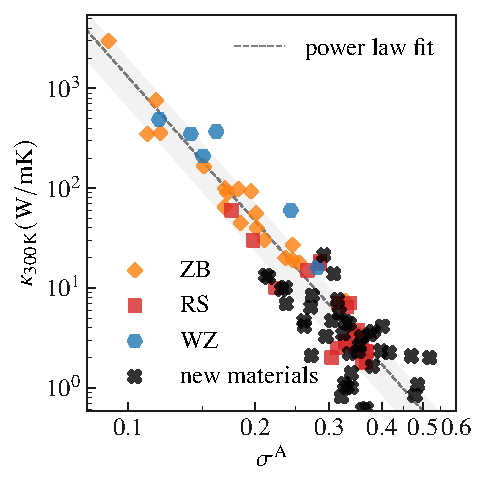
\includegraphics[width=\textwidth]{./data/plots/anharmonicity/9_kappa/incl_computations/sigma_vs_kappa_annot_comp_margin.pdf}
	\caption{
%	\mscomment{too crowded}
	Thermal conductivity at room temperature vs. anharmonicity measure. ZB: zincblende, RS: rock salt, WZ: wurtzite, cf. Fig.\,\ref{fig:anh.kappa}.}
	\label{fig:kappa_sigma_exp_comp}
\end{marginfigure}
%
\begin{marginfigure}
	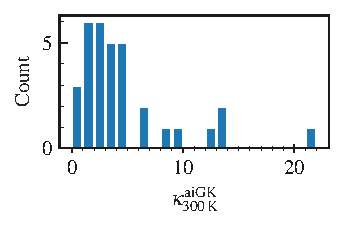
\includegraphics[width=\textwidth]{./data/plots/kappa_histogram/histogram.pdf}
	\caption{Summary of the range of thermal conductivities for materials without experimental reference found in this study.}
	\label{fig:kappa_wo_exp_hist}
\end{marginfigure}


\section{New materials and relation to anharmonicity}
\label{sec:results.new}
After validating the aiGK method against experimental literature, we present results for 33~materials \emph{without} experimental reference. We display these values in the context of the $\kappa$ vs. $\sigmaA$ plot introduced in Fig.\,\ref{fig:anh.kappa}, where we identified a power-law relation of experimental thermal conductivities with the anharmonicity measure $\sigmaA$ for simple elementary and binary materials. We show the data again in Fig.\,\ref{fig:kappa_sigma_exp_comp}, but this time including the additional, non-experimentally measured materials computed in this work.
%
It is apparent that the correlation between thermal conductivity $\kappa$ and $\sigmaA$ carries over from the simple materials to the more complex binary and ternary compound classes studied in this work, since the power-law fit in Fig.\,\ref{fig:kappa_sigma_exp_comp} is still performed with respect to the experimental values initially presented in Fig.\,\ref{fig:anh.kappa}. While the overall trend of decreasing thermal conductivity with increasing anharmonicity is clearly preserved, the spread of $\kappa$ values for materials with similar $\sigmaA$ or vice versa increases, which is expected due to the increased structural and chemical complexity of the studied materials.

Focusing on the new materials, we show a zoomed-in part of the $\kappa-\sigmaA$ plane in Fig.\,\ref{fig:kappa_sigma}, with only computational data, highlighting the materials where no experimental reference is available.
%
\begin{figure*}
	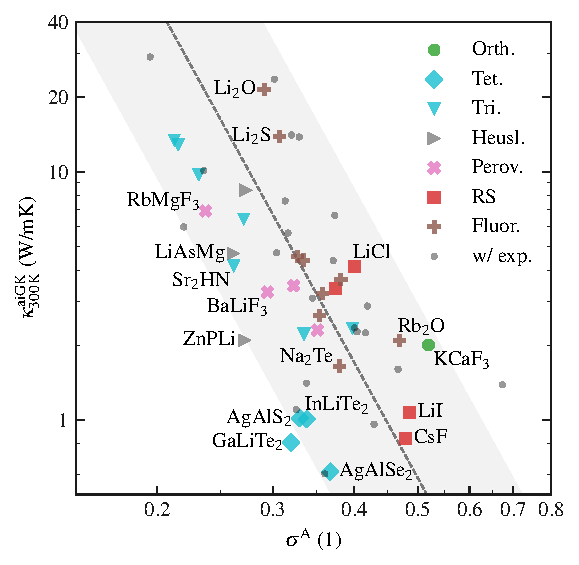
\includegraphics[width=.49\textwidth]{./data/plots/kappa_vs_sigma_trusted/kappa_vs_sigma_trusted.pdf}
	\hfill
	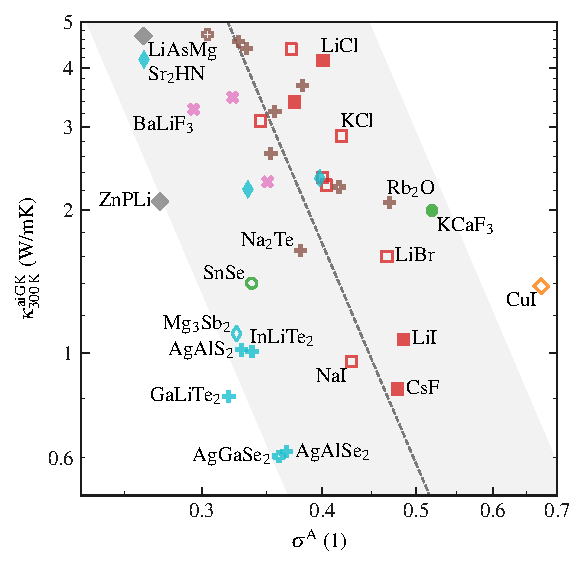
\includegraphics[width=.49\textwidth]{./data/plots/kappa_vs_sigma_trusted/kappa_vs_sigma_trusted_experiment_zoom.pdf}
	\caption{
	Thermal conductivity at room temperature computed via \emph{ab initio} Green Kubo (aiGK) vs. anharmonicity measure. Filled symbols denote materials without experimental reference. Left: Overview of studied materials without experimental reference. Materials with experimental reference are included as small dots for reference. Right: Zoom into the region $\kappa \leq 5$\,W/mK. Open symbols represent materials where experimental reference is available. The dashed line and shaded area are the same as in Fig.\,\ref{fig:kappa_sigma_exp_comp},~i.\,e.,~they represent a power-law fit to experimental thermal conductivities and a $\pm 50\,\%$ margin.}
	\label{fig:kappa_sigma}
\end{figure*}
%
In particular, we find 28 new materials with a computed bulk thermal conductivity of $\kappa^{\rm aiGK} < 10\,{\rm W/mK}$, 24 of which show $\kappa^{\rm aiGK} < 5\,{\rm W/mK}$, and 8 with $\kappa^{\rm aiGK} \leq 2\,{\rm W/mK}$,~i.\,e.,~comparable to the bulk thermal conductivity of existing and candidate thermoelectric materials such as Bi$_2$Te$_3$ and Bi$_2$Se$_3$ (1.3\,W/mK~\cite{Goldsmid.1956,Satterthwaite.1957}), PbTe (2.0\,W/mK~\cite{Elsharkawy.1983}), SnSe (1\,W/mK~\cite{Zhao.2014,Wei.2016,Sassi.2014}), M$_2$Sb$_3$ (2.3\,W/mK~\cite{Ahmadpour.2007,Pan.2020}), or GeTe (2.5\,W/mK~\cite{Perumal.2015}). A full list of all values is given in Tab.\,\ref{tab:kappa.noexp}, and a histogram of the values is shown in Fig.\,\ref{fig:kappa_wo_exp_hist}. The materials of very low thermal conductivity comprise simple binary, cubic materials such as the rock salt structures CsF ($\kappa^{\rm aiGK} = 0.84$) and LiI ($\kappa^{\rm aiGK} = 1.07$), or the fluorite structure Na$_2$Te ($\kappa^{\rm aiGK} = 1.64$), but also more complex structures such as the strongly anharmonic perovskites KCdF$_3$ ($\kappa^{\rm aiGK} = 1.67$) and KCaF$_3$ ($\kappa^{\rm aiGK} = 2.00$).


\subsection{Chalcopyrite systems}
\label{sec:chalcopyrites}
Particularly noteworthy is a class of ternary materials, so-called \emph{chalcopyrites}, a tetragonal crystal class closely related to the zincblende structure~\cite{Wasim.1979}. These crystals have been studied in the past primarily because of their non-linear optical properties~\cite{Ho.2014}, but also thermal transport properties have been studied~\cite{Spitzer.1970,Wasim.1979,Garbato.1979}, mainly because thermal transport can limit the optical efficiency in these devices~\cite{Beasley.1994}. However, experimental references for this class of materials are scarce, and do not agree well~\cite{Beasley.1994}. 
%
\begin{table}[ht]
  \centering
  \fontfamily{ppl}\selectfont
  \begin{tabulary}{\textwidth}{LC}
    \toprule
    Reference & Thermal conductivity at 300\,K (W/mK) \\
    \midrule
    Berger 1966 (experiment)~\cite{berger1969}   & $2.7$          \\
    Beasley 1995 (experiment)~\cite{Beasley.1994} & $1.1$          \\
    This work (theory)                           & $0.6 \pm 0.2$  \\
    \bottomrule
    \vspace{.5em}
  \end{tabulary}
  \caption{Overview of experimental references for AgGaSe$_2$.}
  \label{tab:exp.aggase2}
\end{table}
%
Picking AgGaSe$_2$ as an example, there are two distinct measurements available as summarized in Tab.\,\ref{tab:exp.aggase2}, ranging from $1.1-2.7$\,W/mK~\cite{Beasley.1994,berger1969}. These values are complemented by calculated values based on semi-empirical models, ranging from $4.8-9.0$\,W/mK~\cite{Wasim.1979,Rincon.1995}. Our computed thermal conductivities are collected in Tab.\,\ref{tab:exp.chalcopyrites}.
%
\begin{table}[ht]
  \centering
  \fontfamily{ppl}\selectfont
  \begin{tabularx}{\textwidth}{lXcXc}
    \toprule
    Material & & $\kappa^{\rm aiGK}$ (W/mK) & & $\sigmaA$ \\
    \midrule
	  AgAlS$_2$   & & $1.01 \pm 0.20$ & & 0.33 \\
          AgAlSe$_2$  & & $0.62 \pm 0.16$ & & 0.37 \\
          AgGaSe$_2$  & & $0.61 \pm 0.18$ & & 0.35 \\
          GaLiTe$_2$  & & $0.81 \pm 0.15$ & & 0.31 \\
          InLiTe$_2$  & & $1.01 \pm 0.26$ & & 0.33 \\
    \bottomrule
    \vspace{.5em}
  \end{tabularx}
  \caption{Overview of computed thermal conductivities for chalcopyrite materials.}
  \label{tab:exp.chalcopyrites}
\end{table}

Besides AgGaSe$_2$, there is experimental reference for the chemically closely related material, AgGaS$_2$, with a measured thermal conductivity of 1.4\,W/mK~\cite{Beasley.1994}.
%\footnote{While we included AgGaS$_2$ in our dataset, we needed to discard the material because of aiMD convergence problems. 
%\mscomment{what kind of problems?}
%However, we like to mention this material in the context of this study as potentially interesting material for future investigations.} 
While our computational data might underestimate the thermal conductivity in these compounds slightly\footnote{Please keep in mind, that the absolute errors are only of the order of 0.5-1\,W/mK.}, we nevertheless see a clear indiciation of very low intrinsic thermal conductivity in AgGaSe$_2$, and the chemically closely related compounds AgAlS$_2$ and AgAlSe$_2$. At least regarding their thermal transport properties, they are therefore comparable or even superior to the existing thermoelectric materials listed in the previous section, while being free of heavy metals such as Pb or Bi.
The class of chalcopyrite materials has recently been investigated in a high-throughput study conducted by Plata and coworkers~\cite{Plata.2021pre}. Their findings are overall in line with ours, supporting the finding that the class of chalcopyrite materials may comprise several promising thermal insulators.
 % Mg$_3$Sb$_2$~\cite{kajikawa2003,Condron.2006,Zhang.2009,Zhang.2018,Pan.2020,Ding.2021}.
%\todo{$\kappa_{\rm MgSb}^{\rm aiGK} = 1.10 \pm 0.26$}

To qualitatively elucidate the nuclear dynamics of the chalcopyrite systems, we present phonon spectral functions obtained from a temperature dependent model Hamiltonian for the nuclear system up to third-order displacements to estimate phonon-phonon interactions in Fig.\,\ref{fig:sqe_all}~\cite{Hellman.2013,Hellman.2013b,Squires}.
%
\begin{figure}
	\centering
	AgGaSe2$_2$ \hspace{3.7cm} AgAlSe$_2$\\
	% \includegraphics[width=0.49\textwidth]{./data/plots/spectral_functions/122.04.AgGaS2.12.png}
	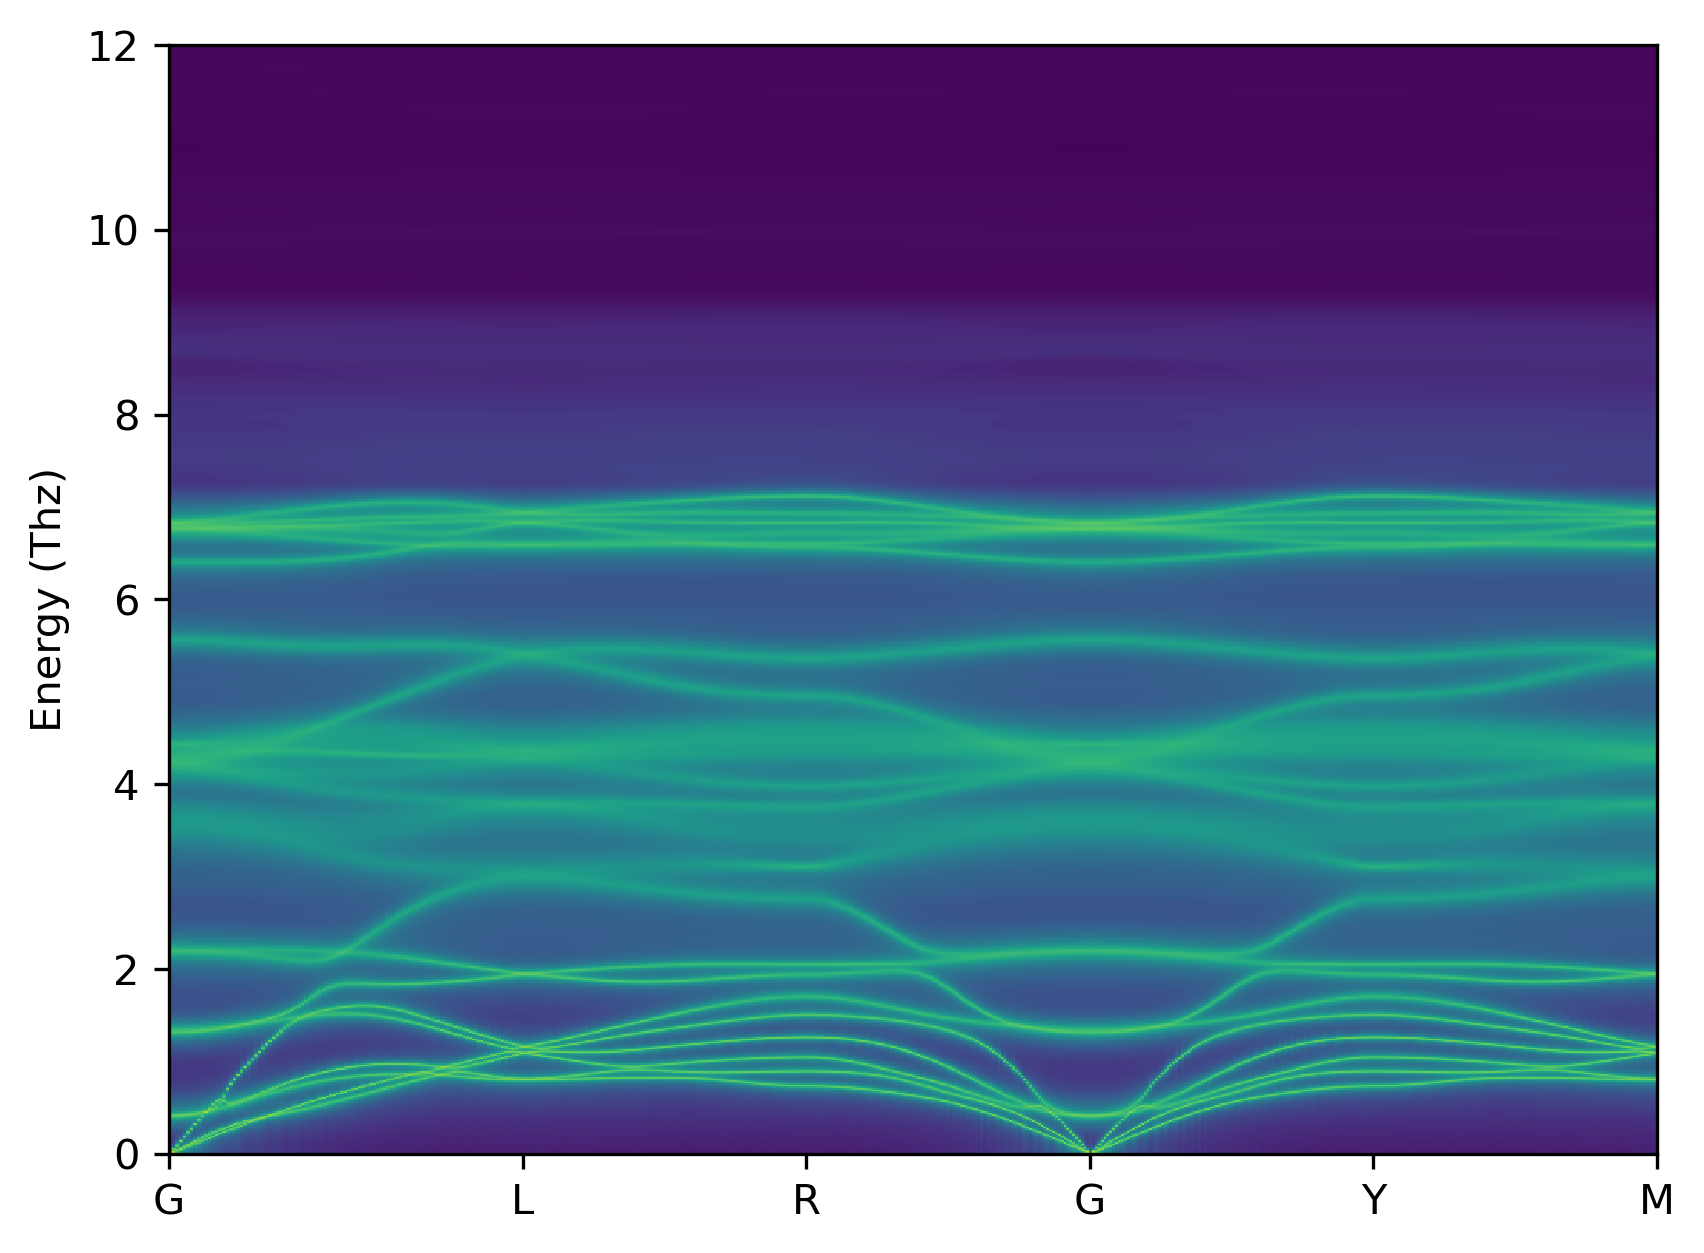
\includegraphics[width=0.49\textwidth]{./data/plots/spectral_functions/122.04.AgGaSe2.12.png}
	%	AgAlS$_2$ \hspace{3.7cm} AgAlSe$_2$\\
	%\includegraphics[width=0.49\textwidth]{./data/plots/spectral_functions/122.04.AgAlS2.15.png}
	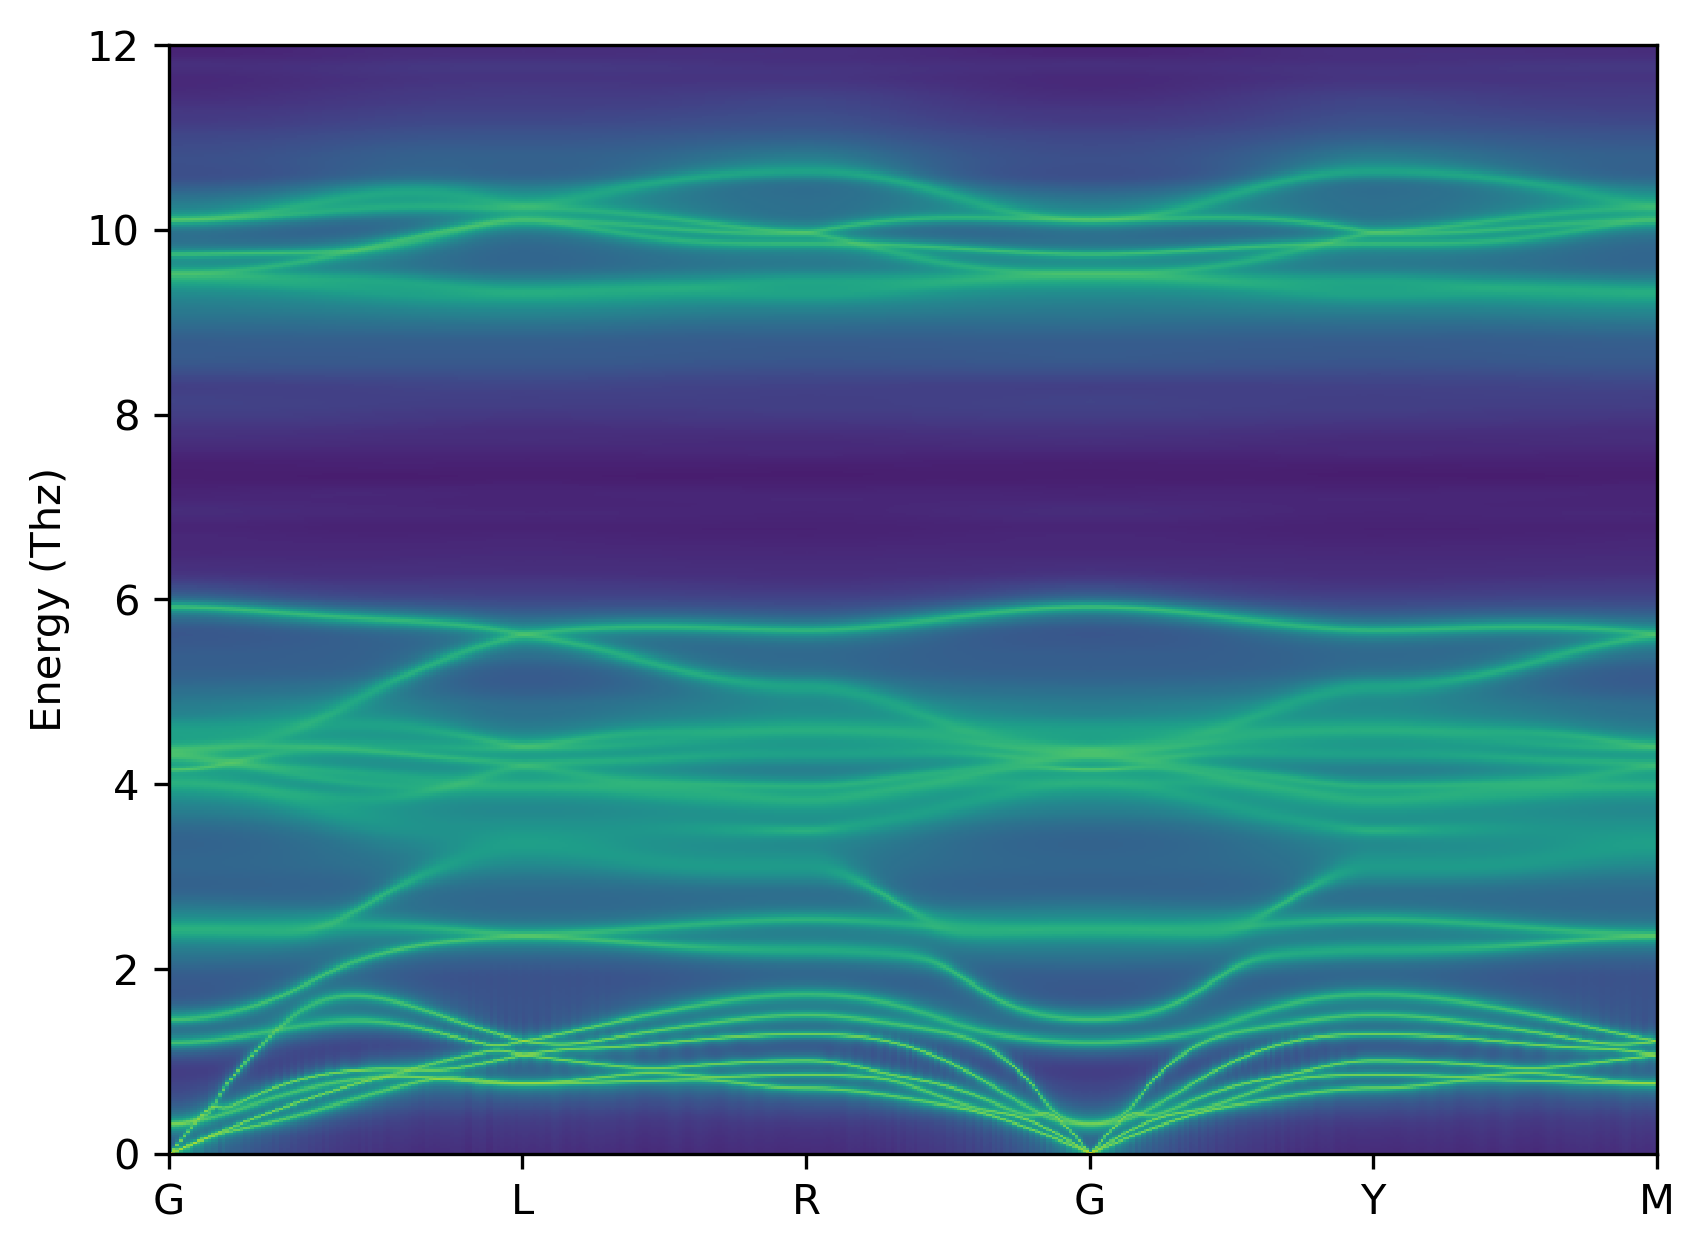
\includegraphics[width=0.49\textwidth]{./data/plots/spectral_functions/122.04.AgAlSe2.12.png}
	\\
	GaLiTe$_2$ \hspace{3.7cm} InLiTe$_2$\\
	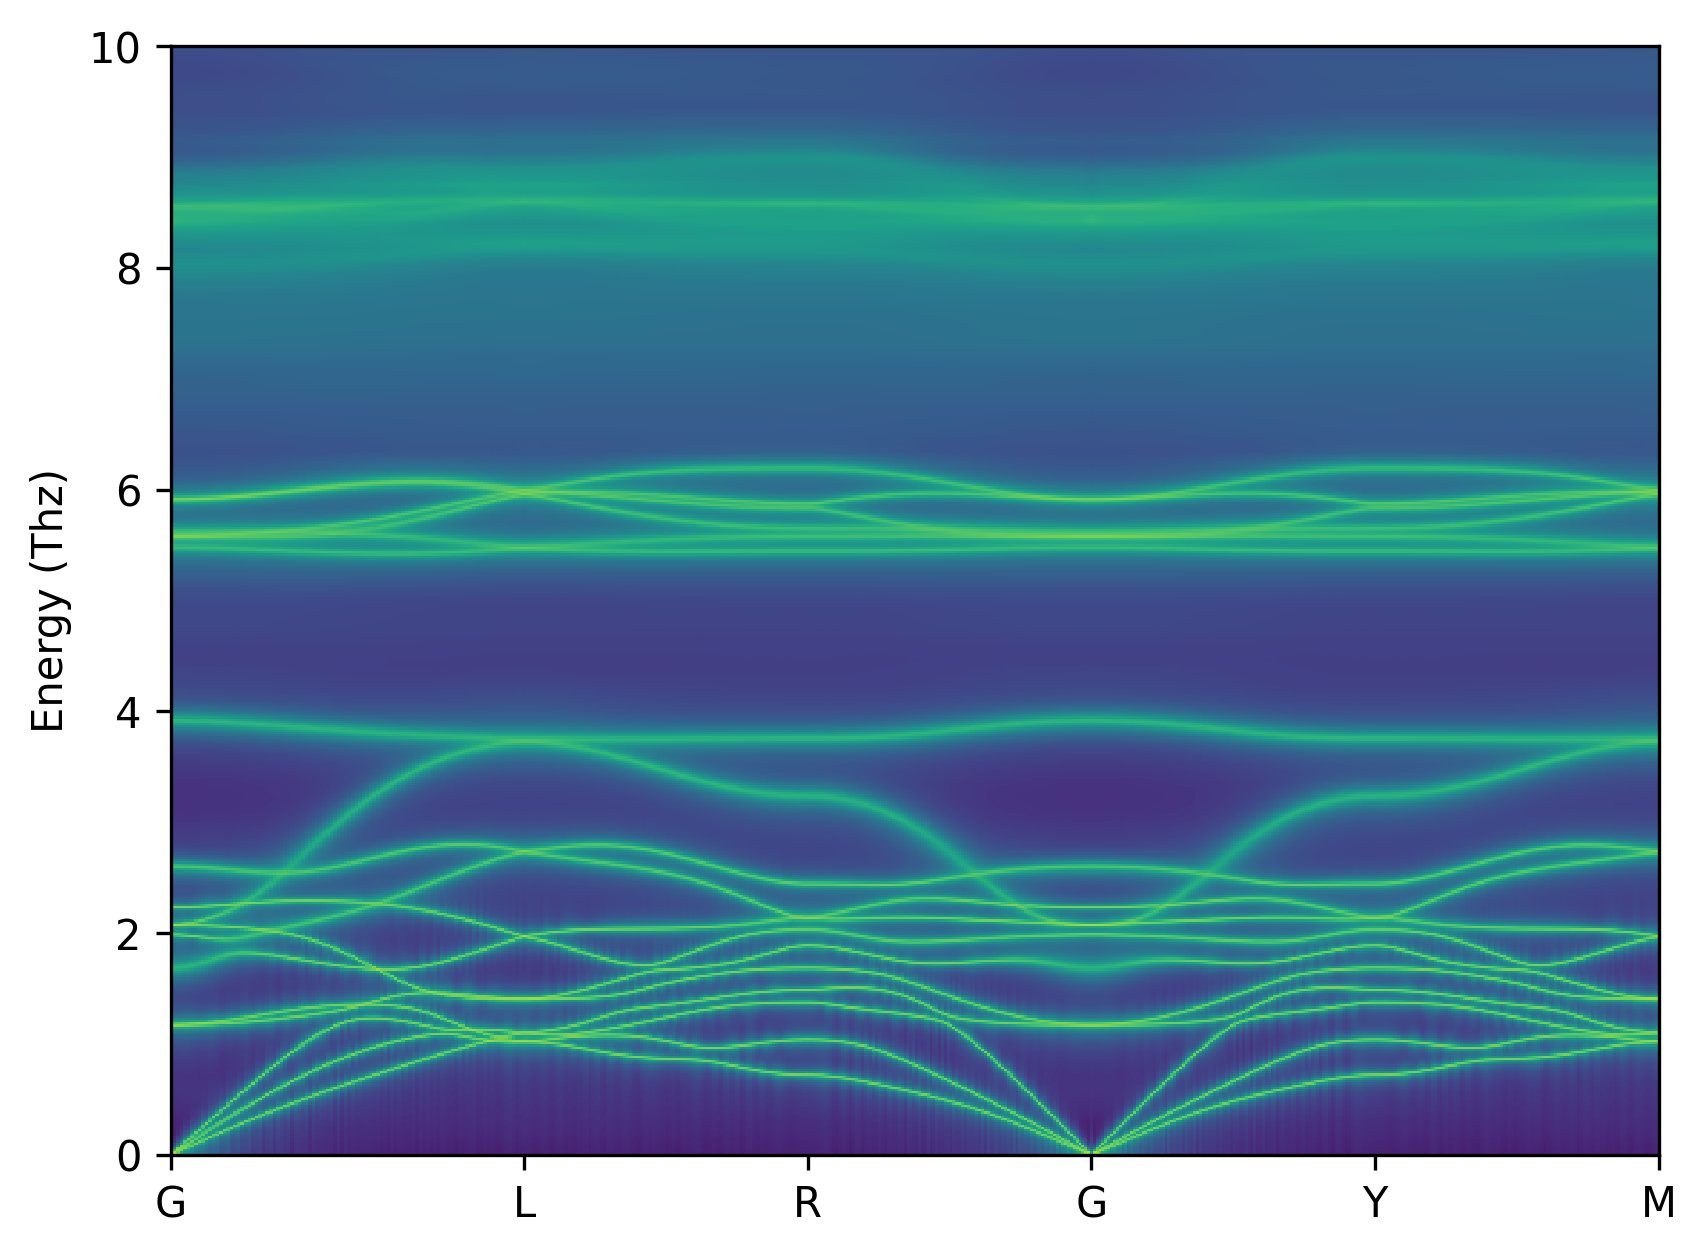
\includegraphics[width=0.49\textwidth]{./data/plots/spectral_functions/122.04.GaLiTe2.png}
	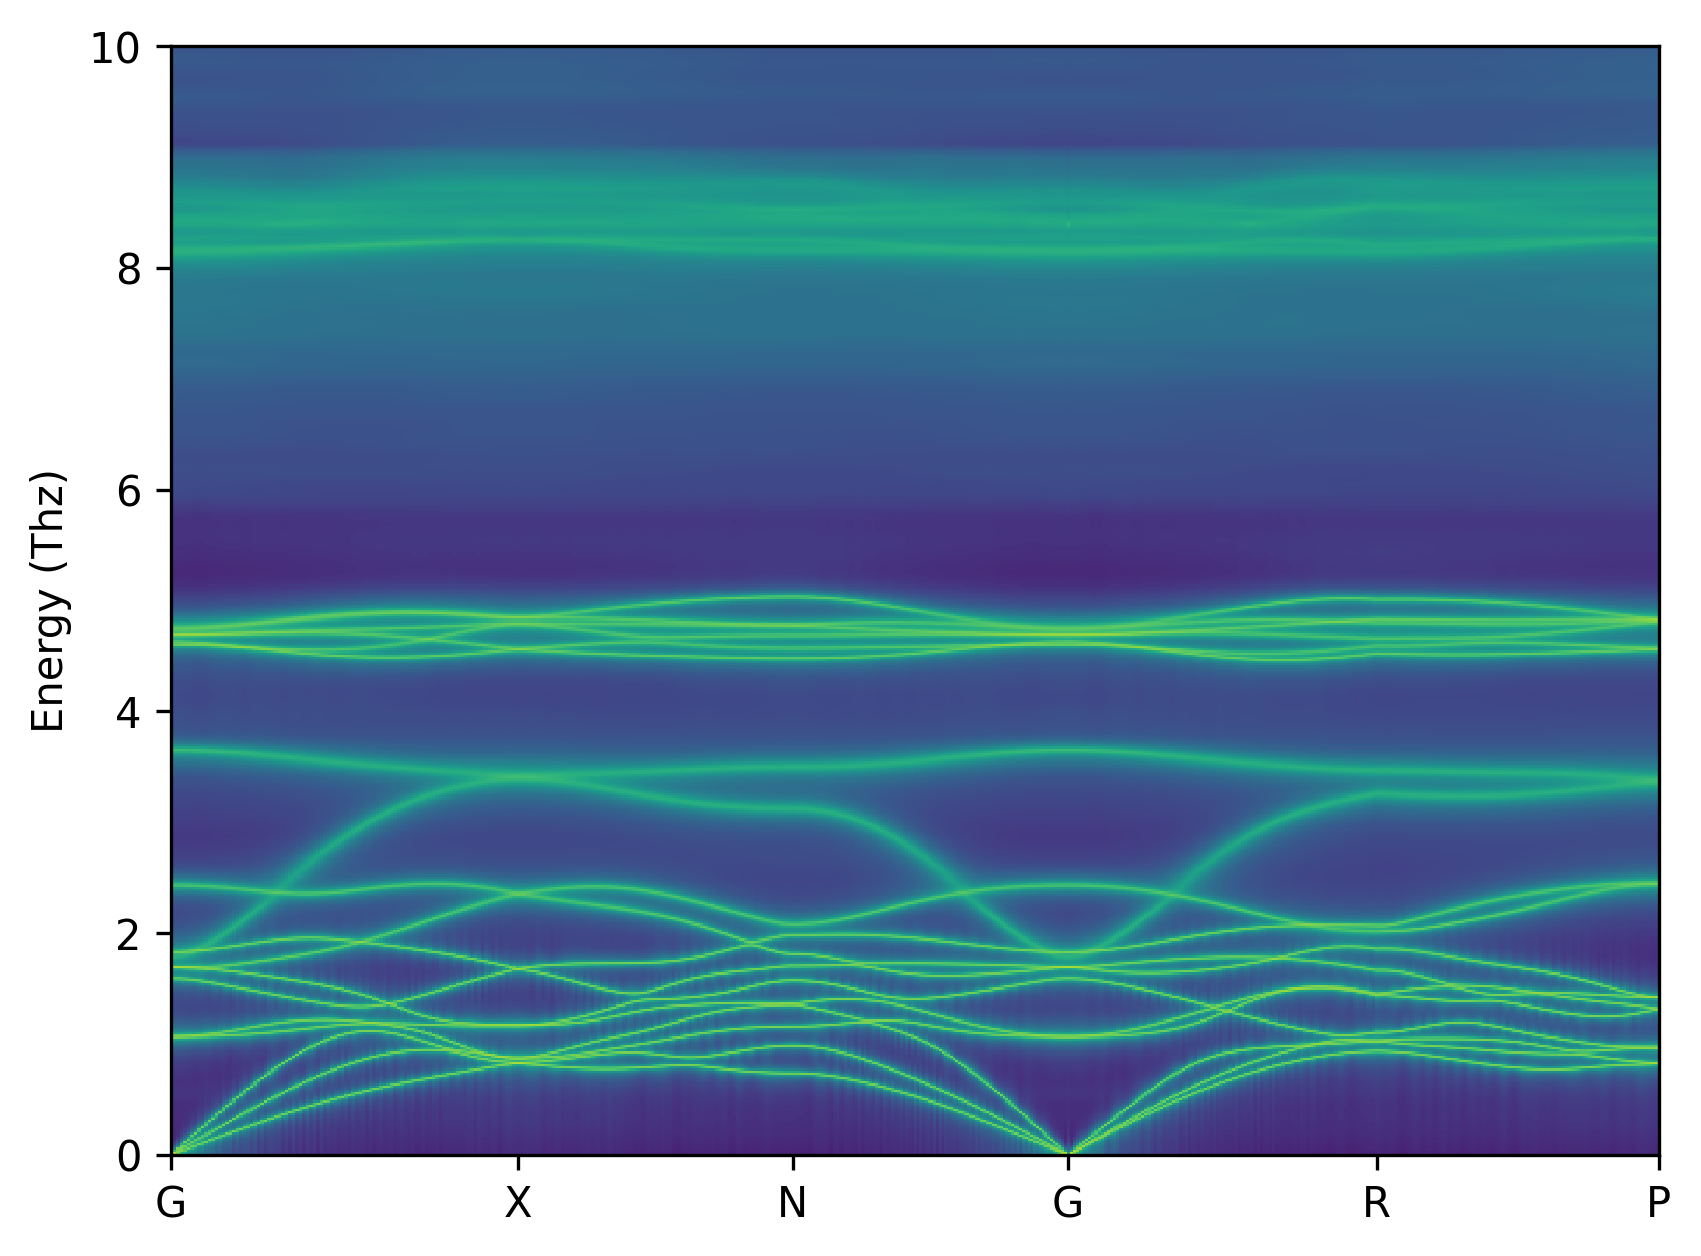
\includegraphics[width=0.49\textwidth]{./data/plots/spectral_functions/122.04.InLiTe2.png}
	\caption{Spectral functions for the chalcopyrite materials, AgGaSe$_2$, AgAlSe$_2$, GaLiTe$_2$, and InLiTe$_2$.}
	\label{fig:sqe_all}
\end{figure}
%
The common feature of these dispersions are the very flat acoustic branches which vary less than 1\,THz across the entire Brillouin zone, and a multitude of flat, nearly degenerate optical branches showing very litte to no dispersion. From a phonon-theory point of view, non-dispersive branches correspond to localized atomic motion in the system and therefore carry little heat beyond the Einstein-like diffusion of thermal energy from atom to atom, which is the dominant heat transport mechanism in structurally disordered systems like glasses~\cite{Simoncelli.2019}. Furthermore, in particular the optical branches are substantially broadened, which corresponds to strong anharmonic coupling in these systems, reducing their thermal conductivity.
%
\begin{table}[ht]
  \centering
  \fontfamily{ppl}\selectfont
\begin{tabularx}{\linewidth}{rXXX}
\toprule
Space group  &    material & $\kappa^{\rm aiGK}$ (W/mK) & $\sigmaA$  \\
\midrule
         122 & AgAlSe$_2$ &             0.62 &       0.37 \\
         122 & GaLiTe$_2$ &             0.81 &       0.32 \\
         225 &        CsF &             0.84 &       0.48 \\
         122 & InLiTe$_2$ &             1.01 &       0.34 \\
         122 &  AgAlS$_2$ &             1.01 &       0.33 \\
         225 &        LiI &             1.07 &       0.49 \\
         225 &   Na$_2$Te &             1.64 &       0.38 \\
          62 &   KCdF$_3$ &             1.67 &       0.53$^\dagger$ \\
          62 &   KCaF$_3$ &             2.00 &       0.52 \\
         225 &    Rb$_2$O &             2.08 &       0.47 \\
         216 &      ZnPLi &             2.09 &       0.27 \\
         166 & InNaSe$_2$ &             2.22 &       0.34 \\
         221 &  CsCdF$_3$ &             2.30 &       0.35 \\
         166 & InLiSe$_2$ &             2.34 &       0.40 \\
         225 &   Na$_2$Se &             2.63 &       0.35 \\
         225 &   Li$_2$Te &             3.24 &       0.36 \\
         221 &  BaLiF$_3$ &             3.27 &       0.29 \\
         225 &         KH &             3.39 &       0.37 \\
         221 &  RbZnF$_3$ &             3.47 &       0.32 \\
         225 &     K$_2$O &             3.67 &       0.38 \\
         225 &       LiCl &             4.14 &       0.40 \\
         166 &   Sr$_2$HN &             4.17 &       0.26 \\
         225 &    Na$_2$S &             4.40 &       0.33 \\
         225 &   Li$_2$Se &             4.55 &       0.33 \\
         216 &     LiAsMg &             4.67 &       0.26 \\
         166 &  LiScS$_2$ &             6.42 &       0.27 \\
         221 &  RbMgF$_3$ &             6.94 &       0.24 \\
         216 &      LiNZn &             8.42 &       0.27 \\
         166 &  InNaO$_2$ &             9.71 &       0.23 \\
         166 &  CuGaO$_2$ &            12.82 &       0.22 \\
         166 &  LiRhO$_2$ &            13.37 &       0.21 \\
         225 &    Li$_2$S &            13.85 &       0.31 \\
         225 &    Li$_2$O &            21.39 &       0.29 \\
\bottomrule
\end{tabularx}
  \caption{Bulk thermal conductivities for materials without experimental reference. $\dagger$: The anharmonicity measure for KCaF$_3$ is increased when the entire simulation is taken into account with $\sigmaA \approx 1.32$, since the simulation is close to a structural phase transition. We observe jumps in $\sigmaA (t)$ similar to those discussed for KCaF$_3$ in Sec.\,\ref{chp:anharmonicity}, but more pronounced. When KCdF$_3$ is close to the orthorombic reference, $\sigmaA \approx 0.53$. Structural phase transition are known to occur in KCdF$_3$ at around 470\,K~\cite{Hidaka.1977,Hidaka.1990}.}
  \label{tab:kappa.noexp}
\end{table}

\section{Conclusion}
We have estimated the convergence of aiGK simulations in terms of an effective simulation time focusing on the slow degrees of freedom of the system, and validated the approach against experimental values from the literature. In total, we computed thermal conductivities for 57 materials and verified our screening approach in terms of the anharmonicity measure $\sigmaA$. We found that the overall trend of decreasing thermal conductivity when anharmonicity increases initially inferred from the set of simple compounds carried over qualitatively to the more complex bulk materials considered in this work. We presented thermal conductivities for 33 materials where experiemental reference is not yet available, and identified the family of chalcopyrite crystals as a potentially interesting class of low thermal conductivity compounds, with several systems showing very low thermal conductivity of $\kappa \approx 1$\,W/mK at room temperature, which is comparable to or even below currently investigated thermoelectric candidates such as SnSe or Mg$_2$Sb$_3$~\cite{Zhao.2014,Wei.2016,Sassi.2014,Pan.2020,kajikawa2003,Condron.2006,Zhang.2009,Zhang.2018,Ding.2021}

%\mscomment{Limits should be discussed before results part.}
%\FK{So far the structure was i) Implementation (what do we do), ii) benchmark (how do we perform, what do we miss), iii) application (what do we find, knowing about possible shortcomings).}



\chapter{Conclusion}

\chapter{Outlook}

\cleardoublepage
\phantomsection
\addcontentsline{toc}{chapter}{Bibliography}

\bibliographystyle{unsrt}
\bibliography{references}

% \setcounter{secnumdepth}{-1}

% part*{appendix}

% \setcounter{tocdepth}{1}
% \addtocontents{toc}{\setcounter{tocdepth}{0}}
\addtocontents{toc}{\protect\setcounter{tocdepth}{0}}
%	\newcommand{\bibsection}{\section{Bibliography}} % <- was missing
\begin{appendices}
%  \appendixpage
  \part*{Appendix}
  \chapter{Bloch Theorem and Brillouin Zone}
\epigraph{\singlespacing \it ``The idea of periodicity in the reciprocal space is useless but, I think, harmless.''}{Paul Gartner}
\section{Bloch Theorem}
\label{sec:BlochTheorem}
The Schr\"odinger equation in 1d reads
\begin{align}
	\hat H \psi (x) = \left( - \frac{\nabla^2}{2m} + V(x) \right) \psi (x) = E \psi (x)~.
	\label{eq:app.bloch.se}
\end{align}
In a periodic potential,
\begin{align}
	V(x + a) = V(x)~,
	\label{eq:app.bloch.potential}
\end{align}
the periodicity can be expressed by stating that the translation operator $\hat T_a$ defined by its action,
\begin{align}
	\hat T_a f(x) = f(x + a)~,
	\label{eq:app.bloch.Ta}
\end{align}
commutes with the Hamiltonian,
\begin{align}
	\left[ \hat H , \hat T_a\right] = 0~.
	\label{eq:app.bloch.commute}
\end{align}
The eigenstates $\psi (x)$ of $\hat H$ are therefore also eigenstates of $\hat T_a$~\cite{Basdevant2000}. The translation operator is unitary, $\D{\hat T}_a = \hat{T}_a^{-1}$, but not hermitian. The eigenvalues $\lambda$ associated with $\hat T_a$ are thus complex numbers. By definition, one has \mbox{$\psi ( x + na ) = \lambda^n \psi(x)$}. Requiring bounded solutions, $\lim_{x \rightarrow \infty} \lvert \psi (x) \rvert < \infty$, imposes the condition $\lvert \lambda \rvert = 1$.
The function $\psi$ can therefore be written as
\begin{align}
	\psi (x) = c(x) u(x)~,
\end{align}
with a real, periodic function
\begin{align}
	u: \mathds R \rightarrow \mathds R
	\quad\text{with}\quad u(x + a) = u(x)~,
\end{align}
and a complex function of unit modulus,
\begin{align}
	c: \mathds R \rightarrow \mathds C
	\quad\text{with}\quad \left\lvert c(x) \right\rvert = 1~.
	\label{eq:app.bloch.c1}
\end{align}
We label each possible solution by the number $k$, then
\begin{align}
	c_k (x) = {\rm e}^{\im k x}
	%% don't impose uniqeness here
	%\quad\text{with}\quad k \in \left[0, \frac{2 \pi}{a} \right)
	\label{eq:app.bloch.c2}
\end{align}
% is a unique map from the domain $x \in [0, a)$ to the complex unit circle $\set{z \in \mathds C : \lvert z \rvert = 1}$. 
is a map from the domain $x \in \mathds R$ to the complex unit circle $\set{z \in \mathds C : \lvert z \rvert = 1}$. 
It then holds that $\hat T_a \psi_k (x) = {\rm e}^{\im k a} \psi(x)$,~i.\,e.,~$\psi_k$ is an eigenfunction of $\hat T_a$ with eigenvalue $\lambda = {\rm e}^{\im k a}$. We formulate the
\begin{thm}[Bloch]
	Solutions to the Schr\"odinger equation~\eqref{eq:app.bloch.se} with a periodic potential of periodicity $a$ are of the form
	\begin{align*}
		\psi_k (x) = {\rm e}^{\im k x} u_k (x)~,
	\end{align*}
	with a real, periodic function $u_k$.
%	 for each $k$ in the first Brillouin zone,
%	\begin{align*}
%		k \in \left[0, \frac{2 \pi}{a} \right)~.
%	\end{align*}
\end{thm}
The theorem is trivially extended to the 3d case by using the multiplication rule
\begin{align}
	\hat{T}_{{\bf a} + {\bf b}} f({\bf x}) = \hat{T}_{\bf a} \hat{T}_{\bf b} f({\bf x}) \equiv f({\bf x} + {\bf a} + {\bf b})~.
\end{align}
A more rigorous proof in terms of representation theory can be found,~e.\,g.,~in~\cite{Dresselhaus2007}.

\section{Brillouin Zone}
\label{sec:BrillouinZone}
We have not yet specified the range of the quantum number $k$. This can be done by requiring the complex function $c_k$ defined in Eq.\,\eqref{eq:app.bloch.c2} to map the interval $x \in [0, a)$ \emph{exactly once} to the unit circle so that $k$ is a \emph{unique} label for the eigenvalues ${\rm e}^{\im k a}$ of the translation operator $\hat T_a$.
We therefore define the
\begin{align}
	\text{Brillouin zone} = \set{k : k \in \left[ - \frac{\pi}{a}, \frac{\pi}{a}\right)}~.
\end{align}
For a wavefunction belonging to $k' = k + G$, where $G$ is an integer multiple of the the reciprocal lattice vector $b = 2\pi / a$, we would find
\begin{align}
	\hat T_a \psi_{k + G} (x) = {\rm e}^{\im k a} \psi_{k + G} (x)~.
\end{align}
They are therefore indistinguishable by the translation operator and we define $\psi_k$ and $\psi_{k+G}$ to be the same function,
\begin{align}
	\psi_k (x) = \psi_{k + G} (x)~.
\end{align}
This is sometimes termed ``periodicity of Bloch functions in reciprocal space''.

\chapter{Born-von Karman Supercell}
To ensure normalizability of the functions $\psi_{{\bf k}l}$, one additionally imposes the \emph{Born-von Karman boundary conditions}
\begin{align}
\psi_{{\bf k}l} ({\bf x} + {\bf A}_i) 
= \psi_{{\bf k}l} ({\bf x})
%\label{eq:dft.Bloch.4}
\end{align}
where each ${\bf A}_i$ is a linear combination of the primitive basis vectors $\set{{\bf a}_i}$,
\begin{align}
{\bf A}_i = S_i^{~j} {\bf a}_j\quad\text{with } S_i^{~j} \in \mathds Z~,
\end{align}
where $S$ is a non-singular matrix with integer elements. The space spanned by the $\set{{\bf A}_i}$ is parallelepiped of volume $V = N \, {\bf a}_1 \cdot ({\bf a}_2 \times {\bf a}_3)$, where $N = \det S$ is the number of unit cells that fit into the enlarged cell. This cell is therefore often called \emph{supercell}, and the matrix $S$ is denoted as a \emph{supercell matrix}.
With the Born-von Karman boundary conditions, the domain of all functions and functionals appearing in the Kohn-Sham equations become restricted to the supercell. The ideal, infinite crystal is obtained in the limit $N \rightarrow \infty$.
Using the periodic boundary condition expressed by Eq.\,\eqref{eq:dft.Bloch.4} in the Bloch functions given by Eq.\,\eqref{eq:dft.Bloch.2}, and the periodicity of the functions $u_{{\bf k} l}$, one finds that
\begin{align}
%	{\rm e}^{\im {\bf k} \cdot ({\bf x} + N_i {\bf a}_i)} u_{{\bf k} l} ({\bf x})
%		&= {\rm e}^{\im {\bf k} \cdot {\bf x}} u_{{\bf k} l} ({\bf x}) \nonumber \\
%	\implies
%		{\rm e}^{\im {\bf k} \cdot  N_i {\bf a}_i} 
%			&= 1 \nonumber \\
%	\implies
{\bf k} \cdot {\bf A}_i
&= 2 \pi m_i\quad\text{with } m_i \in \mathds N \text{ such that } 
\forall i: {\bf k} \cdot {\bf a}_i \leq 2 \pi~.
%\label{eq:dft.Bloch.5}
\end{align}
In total there are $N$ permissible values of $\bf k$ labelled by ${\bf m} = (m_1, m_2, m_3)$ that can be expressed in terms of the \emph{reciprocal lattice vectors}~\cite{Sands2002}
\begin{align}
{\bf B}^i 
= 2 \pi \varepsilon^{ijk} \frac{{\bf A}_j \times {\bf A}_k}{{\bf A}_1 \cdot ({\bf A}_2 \times {\bf A}_3)} ~,
%\label{eq:dft.Bloch.bi}
\end{align}
where $\varepsilon^{ijk}$ denotes the Levi-Civita symbol enforcing the correct ordering of $ijk$. The complete set of $\bf k$-values is
\begin{align}
{\bf k}_{\bf m} 
= \sum_{i=1}^3 m_i {\bf B}^i~.
%\label{eq:dft.Bloch.k_m}
\end{align}
The values of $\bf k$ given by Eq.\,\eqref{eq:dft.Bloch.k_m} are those sampled in real-space simulation in a box of the given size,~i.\,e.,~the \emph{Born-von Karman cell}.

\chapter{Finite Differences Force Constants}
The force constants $\Phi$ can be obtained from first-order derivatives of the potential-energy surface,~i.\,e.,~the forces, by rewriting the second derivative in terms of a finite difference expression,
\begin{align}
\Phi_{I \alpha, J \beta}
= \left.\frac{\partial^{2} \mathcal{V}(\mathbf{R})}{\partial R_{I}^{\alpha} \partial R_{J}^{\beta}}\right|_{\mathbf{R}^{0}}
= - \frac{\partial}{\partial R_I^\alpha} F_{J, \beta}
= - \lim_{\epsilon \to 0}
\frac{F_{J, \beta} (\set{\b R': R^{\prime \alpha}_I = R^{0, \alpha}_I + \epsilon )}}{\epsilon}
~.
\label{eq:FC2_finite}
\end{align}
In practice, atom $I$ is displaced by a small but finite displacement $\epsilon$ in the direction $\alpha$, and the force on all other atoms is recorded. By performing the displacement in all $3N$ degrees of freedom, the $3N \times 3N$ forces can be arranged in a matrix ${\rm F}_{[3N \times 3N]}$, and the displacements can be arranged in a matrix ${\rm U}_{[3N \times 3N]} = \epsilon \mathds 1_{[3N \times 3N]}$. The $3N \times 3N$ force-constants matrix $\Phi$ is obtained by the trivial matrix multiplication
\begin{align}
{\rm F }
&= - \Phi {\rm U} 
= - \epsilon \Phi \mathds 1
\label{eq:finite.diff.1}
\\
\implies
\Phi &= - \frac{1}{\epsilon} {\rm F} \mathds 1~.
\end{align}
%\begin{align}
%	F &= - H U \\
%	\implies
%	H &= - U^{+} F \\
%	F &= \begin{pmatrix} \b F_1, & \cdots, & \b F_{3N} \end{pmatrix}
%\end{align}
If $M > 3N$ displacements are used,~e.\,g.,~because positive and negative displacements $\pm \epsilon$ are used, the force constants can be obtained by solving an overdetermined linear equation of the kind
\begin{align}
{\rm F}_{[3N \times M]} &= - \Phi_{[3N \times 3N]} {\rm U}_{[3N \times M]} \\
\implies
\Phi &= - {\rm F} {\rm U}^{+}~,
\label{eq:phi.pseudo.1}
\end{align}
where ${\rm U}^{+}$ denotes the Moore-Penrose pseudo inverse of the displacement matrix $\rm U$~\cite{Penrose1955,Parlinski1997}.

\newthought{The number of required force calculations} can be reduced by considering the spacegroup symmetry of the crystal. This can be achieved in two ways: First, the symmetry can be used to identify the set of inequivalent displacements from which all other forces can be constructed by the following argument: We define the representation $\Gamma^g$ of a symmetry operation $g$ by its action on the atomic coordinates $\set{\b R_I = \b R_I^0 + \b U_I}$ as
\begin{align}
\b R_I^{g} &\equiv {\Gamma}^g (\b R_I) = { P}^g_{IJ} \b R^0_J + { M}^g \b U_I~,
\label{eq:sym.RI'}
\end{align}	
where $P^g_{IJ}$ is the permutation that relates the reference positions of atom $I$ and atom $J$, and $M^g$ is an orthogonal matrix representing the rotation (or inversion) of the respective displacement. 
\begin{marginfigure}
	\centering
	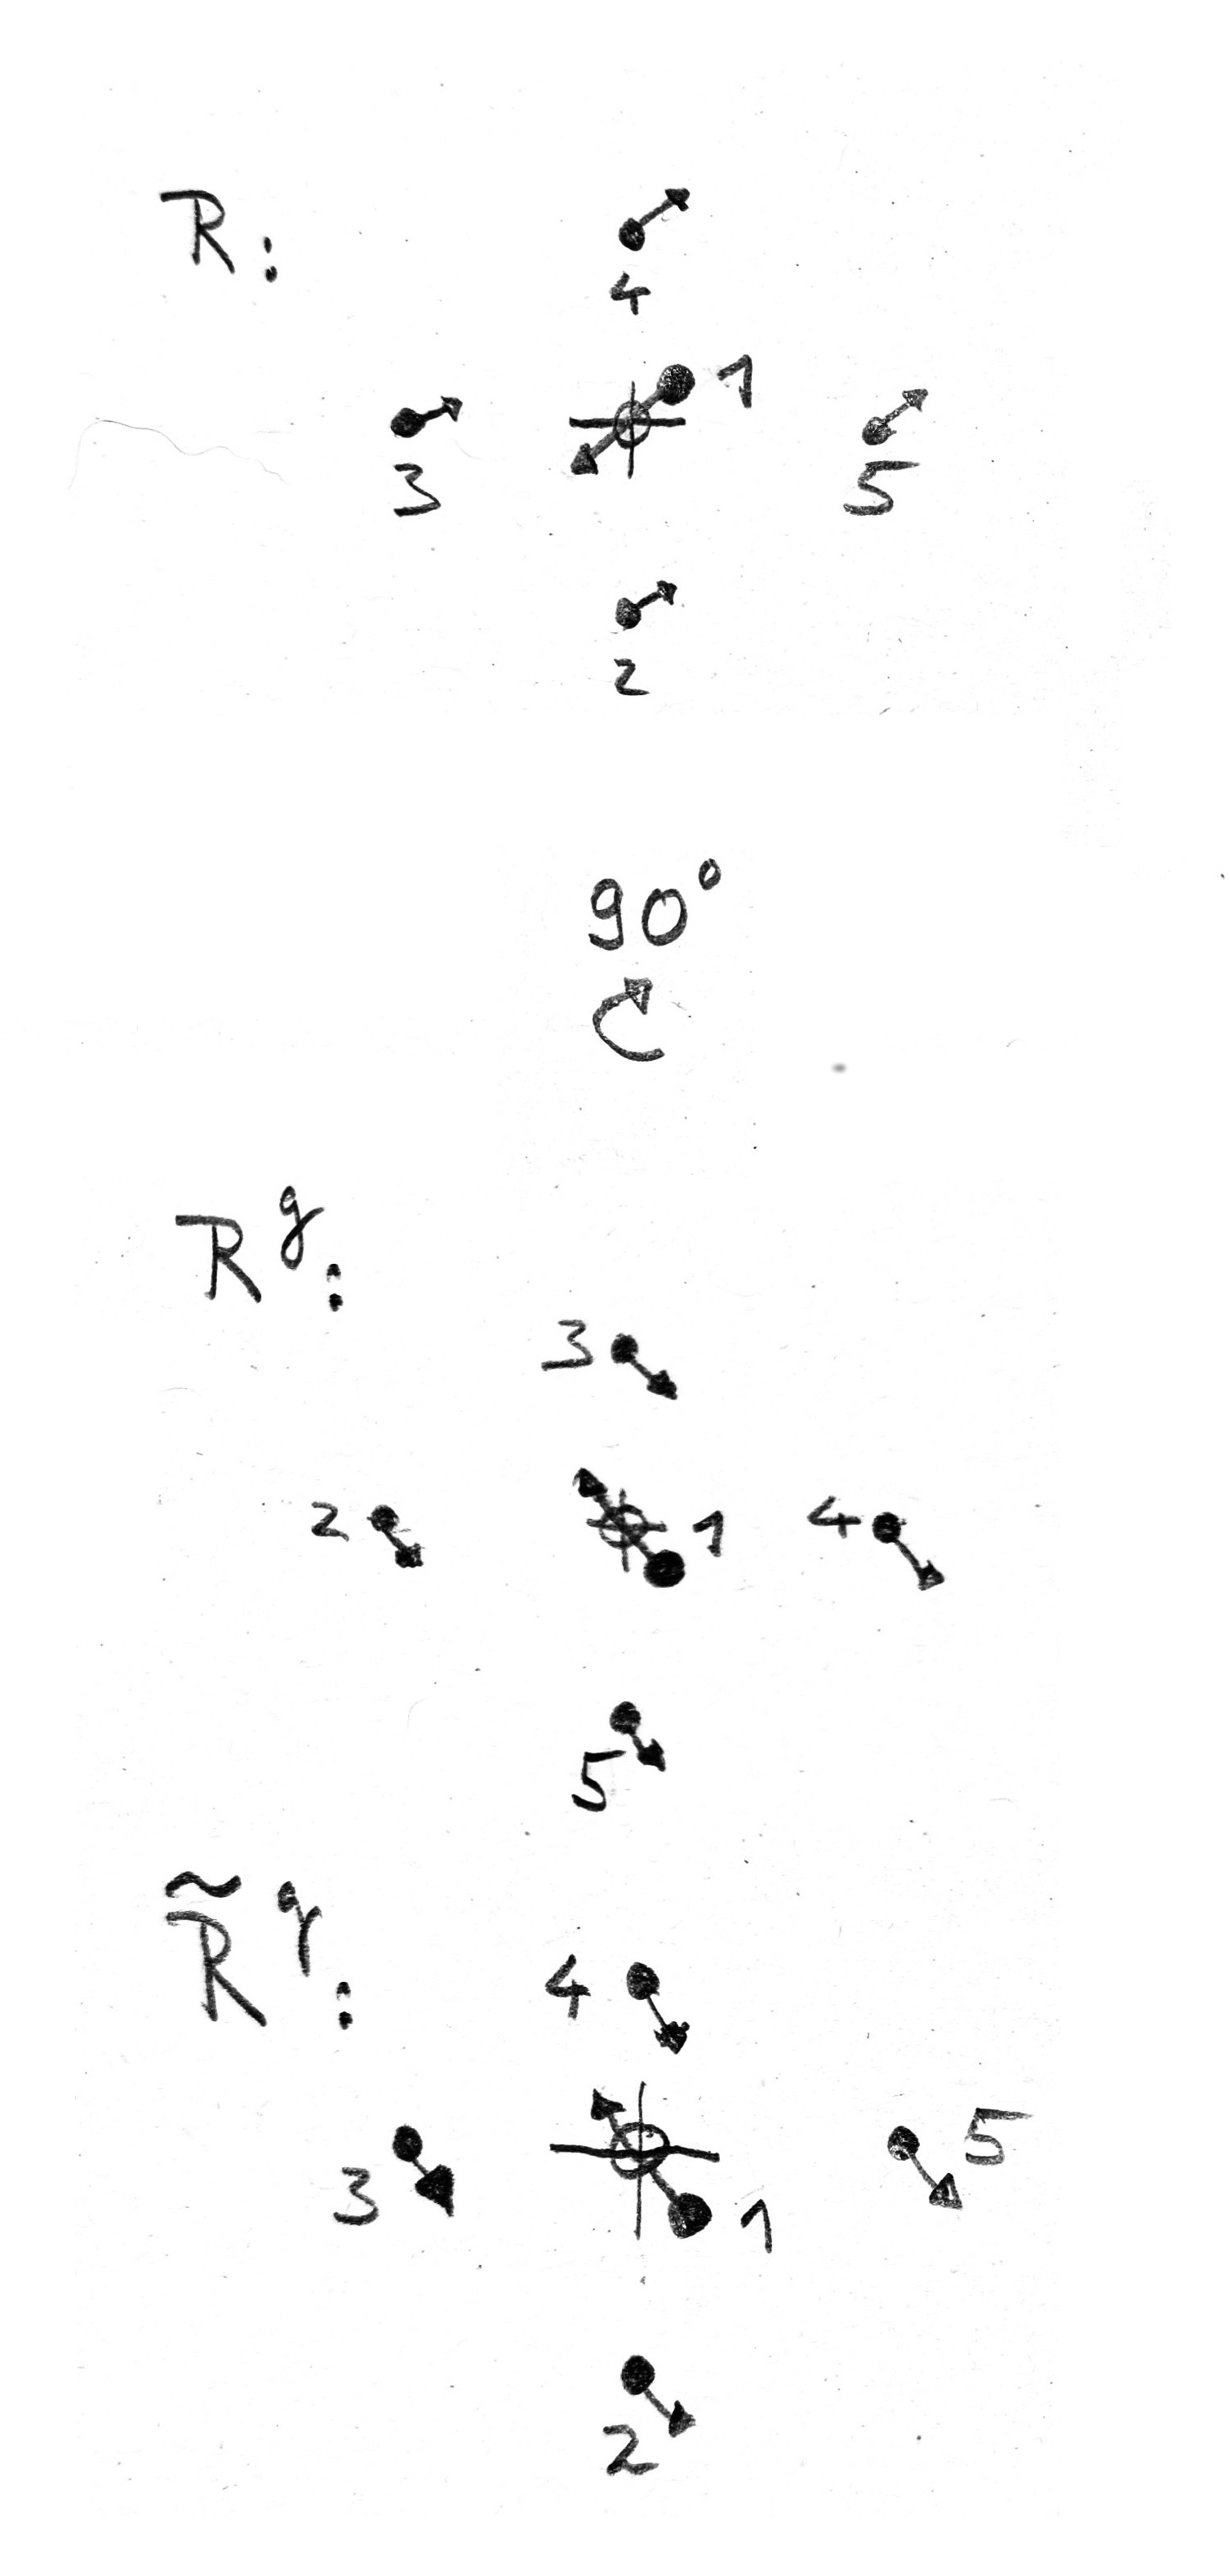
\includegraphics[width=\textwidth]{./data/sketches/symop.jpg}
	\caption{The configurations $\b R$, $\b R^g$, and $\tilde{\b R}^g$ obtained from the symmetry operation $g=\text{90 degrees rotation}$ for a two-dimensional system with five atoms. Arrows indicate the force at each atom.}
	\label{fig:symmetry.1}
\end{marginfigure}
As depicted in Fig.~\ref{fig:symmetry.1}, the forces on each atom in the rotated system $\b R^g = \set{\b R^g_I}$ are obtained by co-rotating the forces in the initial configuration $\b R = \set{\b R_I}$ as
\begin{align}
\b F_I (\b R^g) &= {M}^g \b F_I (\b R)~,
\label{eq:sym.Fp}
\end{align}
i.\,e.,~the forces transform as the displacements $\b U_I$. Let us now define a new configuration $\tilde{\b R}^g$ where just the displacements $\b U_I$ are rotated according to $g$. This can be achieved by rotating the entire system according Eq.\,\eqref{eq:sym.RI'} and applying the inverse permutation $P^{g-1}$,~i.\,e.,
\begin{align}
\tilde{\b R}_I^g 
&= P^{g-1}_{IJ} \b R_I^g 
\stackrel{\eqref{eq:sym.RI'}}{=} \b R^0_I + {\rm M}^g P^{g-1}_{IJ} \b U_J~.
\end{align}
It follows that the force on atom $I$ in the new configuration $\tilde{\b R}^g$ is related to the force in the rotated system $\b R^g$ by this inverse permutation, so that
\begin{align}
\b F_I (\tilde{\b R}^g) 
&= {P}^{g-1}_{IJ} \b F_J (\b R^g) 
= {M}^g  {P}^{g-1}_{IJ} \b F_J (\b R)~.
\label{eq:sym.Ftilde}
\end{align}
By means of this equation, the set of forces obtained for a configuration $\set{\b R_I = \b R_I^0 + \b U_I}$ can be used to generate a set of forces for each symmetrically equivalent configuration $\set{\tilde{\b R}_I^g = \b R_I^0 + {\rm M}^g P^{g-1}_{IJ} \b U_J}$, where $g$ are spacegroup elements.

A complementary approach is to use the symmetry elements $\set{g}$ to reduce the forceconstant matrix to an irreducible basis,
\begin{align}
\Phi 
= \sum_{i=1}^{D} p_i \tilde{\Phi}_i~,
\label{eq:sym.Phi.irrep.1}
\end{align}
where the $\tilde{\Phi}_i$ are \emph{solely} determined by the space group elements $\set{g}$ and analytical properties of the forceconstants, and only the \emph{irreducible components} $p_i$ are system dependent. The pseudoinverse procedure given in Eq.\,\eqref{eq:phi.pseudo.1} then only has to be performed for the $D$ parameters $p_i$~\cite{Parlinski1997}. This procedure can drastically reduce the number of free parameters in the forceconstant matrix. For example, in a $4\times4\times4$ bcc lattice with 128 atoms, $\Phi$ is a matrix with $(3 \cdot 128)^2 = 147456$ elements. However, there are only $D=11$ irreducible parameters $p_i$ that need to be determined~\cite{Hellman2013}.

\TODO{Add the theory for symmetry reduction}

\chapter{Linear Response Distribution Function}
\label{app:lr.f}
To solve for $\Delta f(t)$ defined in Eq.\,\eqref{eq:lr.df.2}, we introduce a shorthand notation such that
\begin{align}
\frac{\d \Delta f}{\d t} = -\im L \Delta f(t) - \im \Delta L (t) f^0~,
\label{eq:lr.df.3}
\end{align}
where the Liouville operator $L^0$ is defined by
\begin{align}
	\im L^0 g = \set{g, H^0}~,
	\label{eq:app.lr.L}
\end{align}
and similarly
\begin{align}
	\im \Delta L (t) g = \set{g, H'(t)}~.
	\label{eq:app.lr.L'}
\end{align}
Equation~\eqref{eq:lr.df.3} is a first order linear differential equation of the form
\begin{align}
	\frac{\d y}{\d t} + p(t) y = q(t)~,
	\label{eq:app.lr.dgl.1}
\end{align}
which is straightforward to solve by using an integrating factor as follows: We identify $y = \Delta f$, $p(t) = \im L^0$, and $q(t) = - \im \Delta L (t) f^0$. Following Ref.~\cite[p.\,68]{Lomen1986}, we define the integrating factor \mbox{$\rho (t) = \exp(\int \d t \, p (t)) = \exp (\im L^0 t)$}, multiply Eq.\,\eqref{eq:lr.dgl.1} with $\rho (t)$, and use that \mbox{$\frac{\d}{\d t} \, \rho(t) = \rho(t) p(t)$} to obtain
$$
\frac{\d}{\d t} (\rho (t) y) = \rho(t) q(t)~.
$$
This gets integrated to
$$
\rho(t) y = \int_{-\infty}^t \d t' \, \rho(t') q(t')
$$
under the boundary condition $y (t \to -\infty) = 0$. In total we obtain
\begin{align}
  y(t) 
    &= \rho^{-1} (t) \int_{-\infty}^t \d t' \, \rho(t') q(t')~, \\
  \implies
  \Delta f(t) 
    &= - {\rm e}^{- \im L^0 t}  \int_{-\infty}^t \d t' \, {\rm e}^{\im L^0 t'} \im \Delta L (t') f^0~.
\end{align}

\chapter{Explicit Formulas}
\section{Harmonic Approximation}
\label{app:ha.formulas}
In Sec.\,\ref{sec:dynmat.periodic}, we introduced the shorthand notation $s=(b, \b q)$, $-s=(b, -\b q)$ to write brief formulas. We give the explicit form of these formulas here.

\newthought{The normal mode coordinates} in the periodic case in terms of complex amplitudes $a^{(\dagger)}_b (\b q)$ read
\begin{subequations}
	\label{eq:u_b(q).amplitudes}
	\begin{align}
	u_b (\b q)
	&=   \frac{1}{\sqrt{2 \omega_b (\b q)}} \left[ \D a_b (- \b q) + \fD a_b (\b q)  \right] \\
	p_b (\b q)
	&= \im \sqrt{\frac{\omega_b (\b q)}{2}} \left[ \D a_b (- \b q) - \fD a_b (\b q)  \right]
	\end{align}
	\end{subequations}
	The inverse relation is given by
	\begin{subequations}
		\label{eq:a(q)}
		\begin{align}
		a_b (\b q)
		&= \sqrt{\frac{\omega_b (\b q)}{2}} u_b (\b q) + \frac{\im}{\sqrt{2 \omega_b (\b q)}} p_b (\b q) \\
		a^\dagger_b (-  \b q)
		&= \sqrt{\frac{\omega_b (\b q)}{2}} u_b (\b q) - \frac{\im}{\sqrt{2 \omega_b (\b q)}} p_b (\b q)
		\end{align}
		\end{subequations}
		The displacements are recovered by
		\begin{align}
		\b u_{i \b L}
		&= \frac{1}{\sqrt{N_{\b q}}} \sum_{b \b q} {\rm e}^{\im  \b q \cdot \b R^0_{i \b L}} \, \b e^\ast_{b i} (\b q) \fD u_b (\b q)
		\label{eq:u_iL}
		% \\
		% \b p_{i \b L}
		% &= \frac{1}{\sqrt{N_{\b q}}} \sum_{b \b q} {\rm e}^{\im  \b q \cdot \b R^0_{i \b L}} \, \b e^\ast_{b i} (\b q) \fD p_b (\b q)
		\end{align}
		%\end{subequations}
		and likewise for $\b p$.
		
		The Hamiltonian reads
		\begin{align}
		\mathcal H (u_b, p_b)
		&= \frac{1}{2} \sum_{b \b q} \left[ p^\ast_b (\b q) p_b (\b q) + \omega^2_b (\b q) u^\ast_b (\b q) u_b (\b q) \right] 
		\end{align}
		Equations of motion
		\begin{align}
		\ddot{u}_b (\b q)
		= \dot{p}_b (\b q)
		= - \frac{\partial \mathcal{H}}{\partial u_b^\ast (\b q)}
		\end{align}

\newpage

\section{Heat Capacity}
\begin{subequations}
\begin{align}
	\beta
		& = \frac{1}{k_{\rm B} T} \\
	c_V 
		&= \frac{\partial E}{\partial T} \\
	E (T)
		&= \sum_s \hbar \omega_s n_s (T) \\
	n_s (T)
		&= \frac{1}{e^{\beta \hbar \omega_s} - 1} \\
	\frac{\partial n_s}{\partial T}
		&= \frac{\hbar \omega_s}{k_{\rm B} T^2} \, n_s (n_s + 1) \\
	\implies c_V
		&= \sum_s \underset{c_{V, s}}{\underbrace{\frac{\hbar^2 \omega_s^2}{k_{\rm B} T^2} \, n_s (n_s + 1)}}
\end{align}
\end{subequations}
Classical limit $k_{\rm B} T \gg \hbar \omega_s$
\begin{subequations}
\begin{align}
	n_s (T) 
		&\to \frac{k_{\rm B} T}{\hbar \omega_s} \gg 1 \\
	\implies E(T)
		&\to 3 N k_{\rm B} T \\
	\implies c_V 
		&\to 3 N k_{\rm B}
\end{align}
\end{subequations}
\end{appendices}

% \backmatter



\end{document}
